\chapter{Selection of neutrino interactions in the ECal}
\label{chap:NeutrinoInteractionSelection}
This analysis presents a measurement of the CC inclusive interaction cross-section of $\nu_\mu$ with lead nuclei using the ND280 \Yoshi{Tracker}{ADDRESSED - I would say that ``Tracker'' is a proper noun, the name of the detector, so it should be capitalised throughout. The detector name is then ``Tracker ECal''} ECals.  To make such a measurement, a sample of neutrino interaction vertices within the ECal must be found.  The selection of events is based on the enhanced reconstruction outlined in chapter~\ref{chap:EnhancedECalReconstruction}, which was specifically designed to \Yoshi{be sensitive to}{ADDRESSED - introduce} track multiplicity.  As a result of this method, vertices in the ECal are naturally separated into topologies defined by the number of reconstructed tracks.  Any selection development should take advantage of this situation and tailor cuts to be specific to each topology, which should result in a higher overall sample purity.  The 3D track matching aspect of the reconstruction was only tuned to handle up to three tracks simultaneously.  However, this analysis aims to measure a CC-inclusive cross-section so it should not be biased against any neutrino energy range.  \Yoshi{There is a deep connection between the number of reconstructed tracks and the energy of the neutrino that created them.  The number of reconstructed tracks should correlate with the number of final state particles involved with the neutrino interaction and the number of final state particles correlates with the energy of the interacting neutrinos.  Therefore it is important to not reject events based solely on the number of reconstructed tracks}{ADDRESSED - state the implied connection between number of prongs and neutrino energy}.  Bearing this information in mind, the selection should separate out the events into the following topologies:
\begin{itemize}
  \item 1 prong topology
  \item 2 prong topology
  \item 3 prong topology
  \item 4+ prong topology
\end{itemize}
The definition of a prong is a reconstructed track associated with a reconstructed vertex.
\newline
\newline
However, as described in section~\ref{sec:ReconOutput}, the output of the enhanced reconstruction has been kept generic and is not specifically tailored to this task.  The reconstruction outputs a set of clusters which contain a set of 3D tracks and every pairwise crossing that said tracks make.  While it is true that in some situations the reconstruction will accurately represent a vertex ``out of the box''---e.g., when only two tracks are reconstructed in the cluster---there will be many situations where extra reconstruction steps are needed before any further selection can take place.  \Yoshi{Hence}{ADDRESSED - I wouldn't start a sentence with ``So,''---it seems like spoken English to me. I'd say ``Hence'' with no comma} the structure of this chapter is as follows: the definition of signal is described first along with the sample used to develop the selection, followed by a discussion of the vertex reconstruction.  After the final reconstruction steps have been discussed, a full discussion of the neutrino selection follows.

\section{Signal definition}
\label{sec:SignalDefinition}
The measurement \Yoshi{that is the intended outcome}{ADDRESSED - ``measurement of this analysis''} of this analysis is the CC inclusive interaction cross-section of $\nu_\mu$ with lead nuclei using the ND280 Tracker ECals.  The active volume of the ECal consists of layers of plastic scintillator and lead absorbers.  Neutrino interactions that occur in the lead absorbers are indistinguishable from those that occur in the plastic scintillator.  Because of this fact, the selection does not attempt to separate the two cases out.  So, the strict signal definition used by this selection  is as follows:
\begin{itemize}
  \item Interacting neutrino is flavour $\nu_\mu$
  \item Interaction type is charged current
  \item Interaction occurs within the active volumes of either the barrel ECal or DS ECal
\end{itemize}
The active volume is defined by the ROOT geometry used in the simulation.  Specifically, it is a rectangular box which encompasses all of the lead and scintillator layers for each ECal module.  Any target element contained within this volume is a signal target.

\section{Monte Carlo sample}
\label{sec:MonteCarloSample}
NEUT was used to generate a neutrino beam sample of Monte Carlo events which corresponds to $3.949\times10^{20}$ POT.  All of this sample was generated using a simulated beam power of 178 kW which is the average beam power used for Run III.  At this intensity, there are an expected 9.46 neutrino interactions per eight bunch spill in ND280.  So, there will be approximately one interaction per bunch across the entire \Yoshi{}{ADDRESSED - was `of'} ND280, meaning the chance of pileup is small. 
\newline
\newline
The sample \Yoshi{described}{ADDRESSED} above only simulated neutrino interactions within ND280 (including the \Yoshi{outermost}{ADDRESSED - was `surrounding'} magnet).  However, we expect many interactions in the surrounding pit (referred to as ``sand interactions'' from now on) to have final states which enter ND280.  So, NEUT was used to generate an additional sample of sand interactions (hereafter referred to as sand Monte Carlo) which corresponds to $3.708\times10^{20}$\Yoshi{~POT}{ADDRESSED}.  There is roughly a 6$\%$ difference in the POT of the beam and sand Monte Carlo.  As the sand Monte Carlo has a sufficiently high level of statistics, scaling the smaller sample to match the larger is acceptable.
\newline
\newline
\begin{table}
  \begin{tabular}{ l r }
    ECal module & No. signal events \\ \hline \hline
    Bottom-right & 223042 \\
    Side-right & 231955 \\
    Top-right & 135476 \\
    Bottom-left & 262500 \\
    Side-left & 293065 \\
    Top-left & 140539 \\
    Downstream & 134100 \\
    \hline
    Total & 1420677 \\
  \end{tabular}
  \caption{The number of signal events in the Monte Carlo sample separated by ECal module.}
  \label{table:NSignalEventsTruth}
\end{table}
The number of signal interactions from the Monte Carlo sample is shown in table~\ref{table:NSignalEventsTruth}, separated into the ECal module they occurred in.  The number of signal interactions is also shown as a function of neutrino energy for the bottom-left, top-right and DS ECals in Fig.~\ref{fig:NSignalEventsTruthNeutrinoEnergy}.  Clearly, there are an extremely high number of signal events in the sample, which means this analysis is in no way statistically limited.  As an example, consider a selection with a 1$\%$ signal efficiency in the DS ECal.  Assuming $100\%$ selected sample purity, the number of selected events would be 1341 which correspond to a statistical error of 2.73$\%$.  Even in this extreme situation, the statistical error is borderline negligible.  It should be clear that any statistical error is this analysis is approximately $0\%$.
\begin{figure}
  \centering
  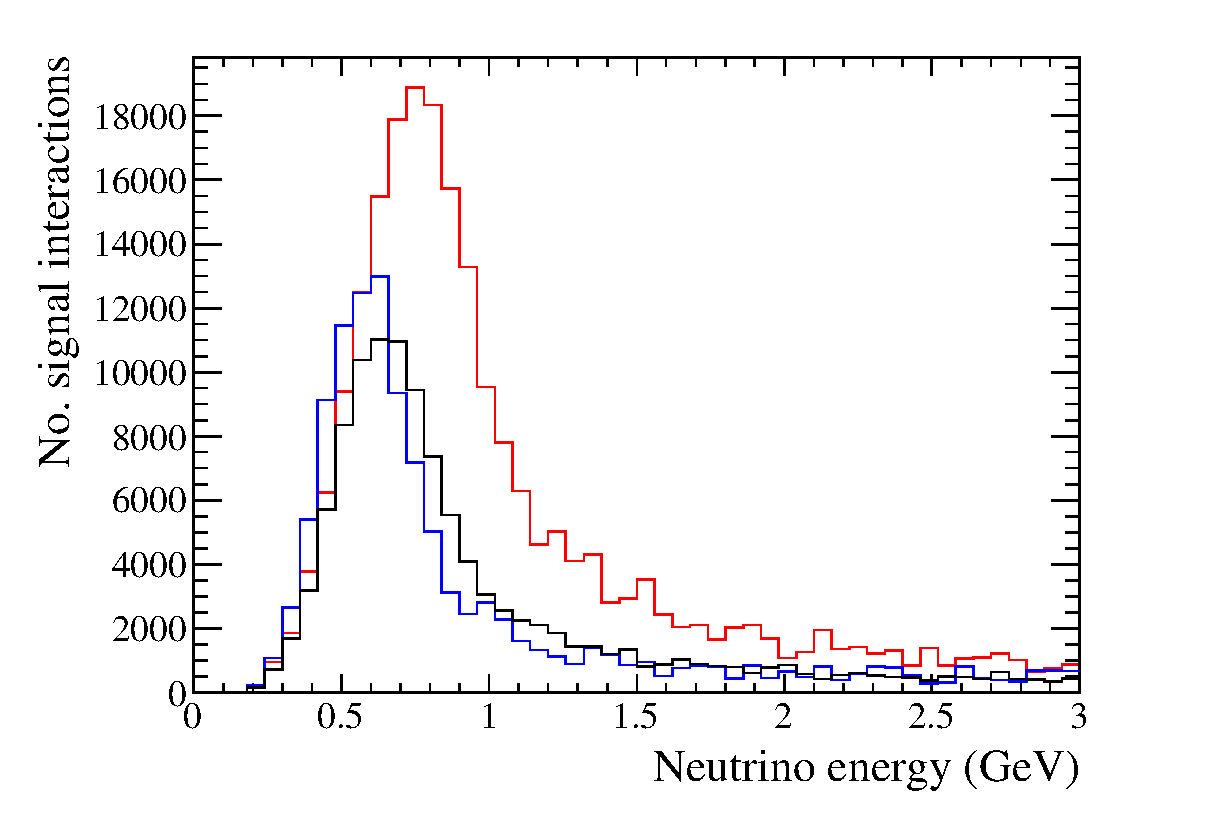
\includegraphics[width=12cm]{images/selection/signal_definition/NSignalEventsNeutrinoEnergy.eps}
  \caption{The number of signal events as a function of neutrino energy in the bottom-left (red), top-right (blue) and DS (black) ECals.}
  \label{fig:NSignalEventsTruthNeutrinoEnergy}
\end{figure}
\section{Vertex reconstruction}
\label{sec:VertexReconstruction}
The output of the enhanced reconstruction already supplies most of the necessary information to reconstruct vertices in the ECal.  As a reminder, the reconstruction outputs a set of ECal clusters which contain the following:
\begin{itemize}
  \item A set of 3D reconstructed tracks
  \item The position at which every pairwise combination of 3D tracks most closely cross (pairwise crossings)
\end{itemize}
The reconstruction makes no quality checks on the 3D tracks in each cluster.  So, the first step is to remove any poorly reconstructed tracks from the cluster.  The need for this step is shown in Fig.~\ref{fig:AngularSeparationNoRejection} which shows the angular separation of reconstructed tracks with the simulated particle which created them, taken from beam Monte Carlo.  While the majority of tracks generally have a small angular separation, Fig.~\ref{fig:AngularSeparationNoRejection} clearly shows a build up of tracks which are offset by 90$^\circ$ to the simulated particles.
\newline
\newline
\begin{figure}%
  \centering
  \subfloat[No track rejection.]{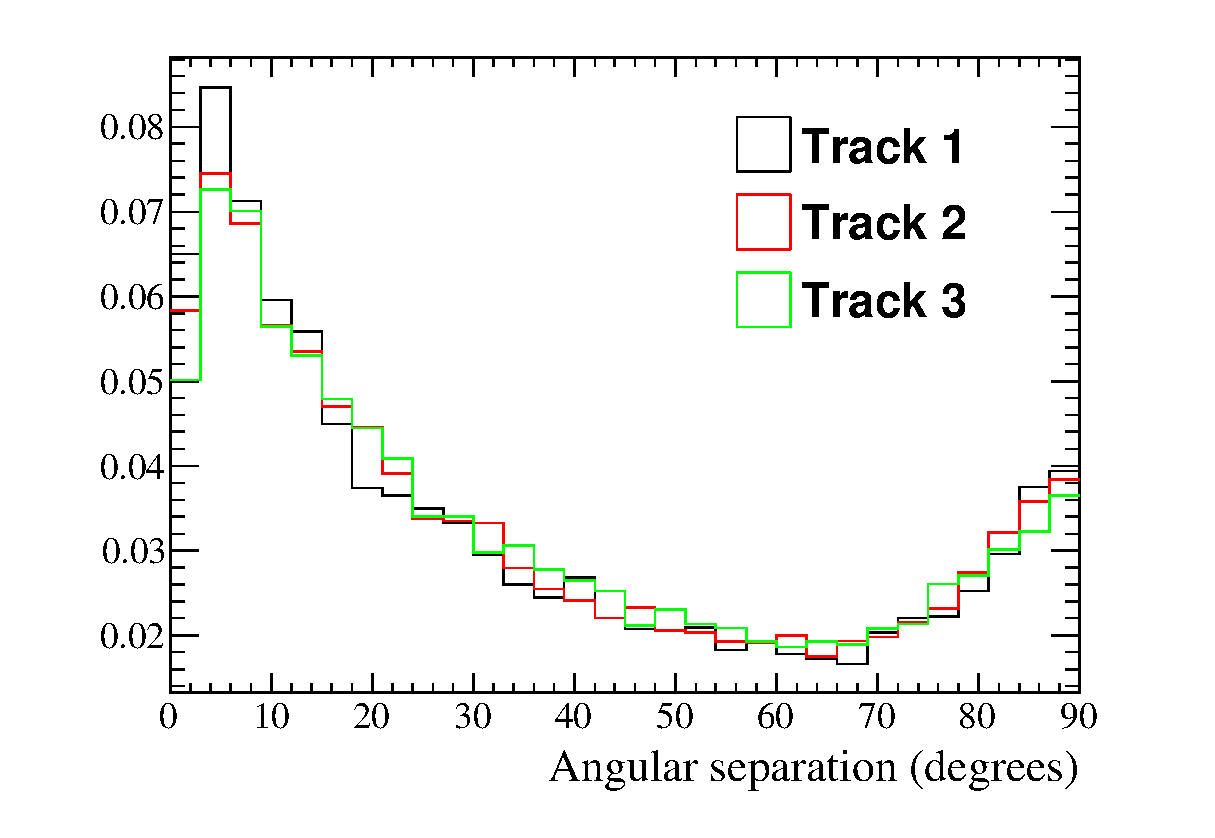
\includegraphics[width=9cm]{images/selection/track_rejection/AngularSeparationNoRejection} \label{fig:AngularSeparationNoRejection}}
  \subfloat[With track rejection.]{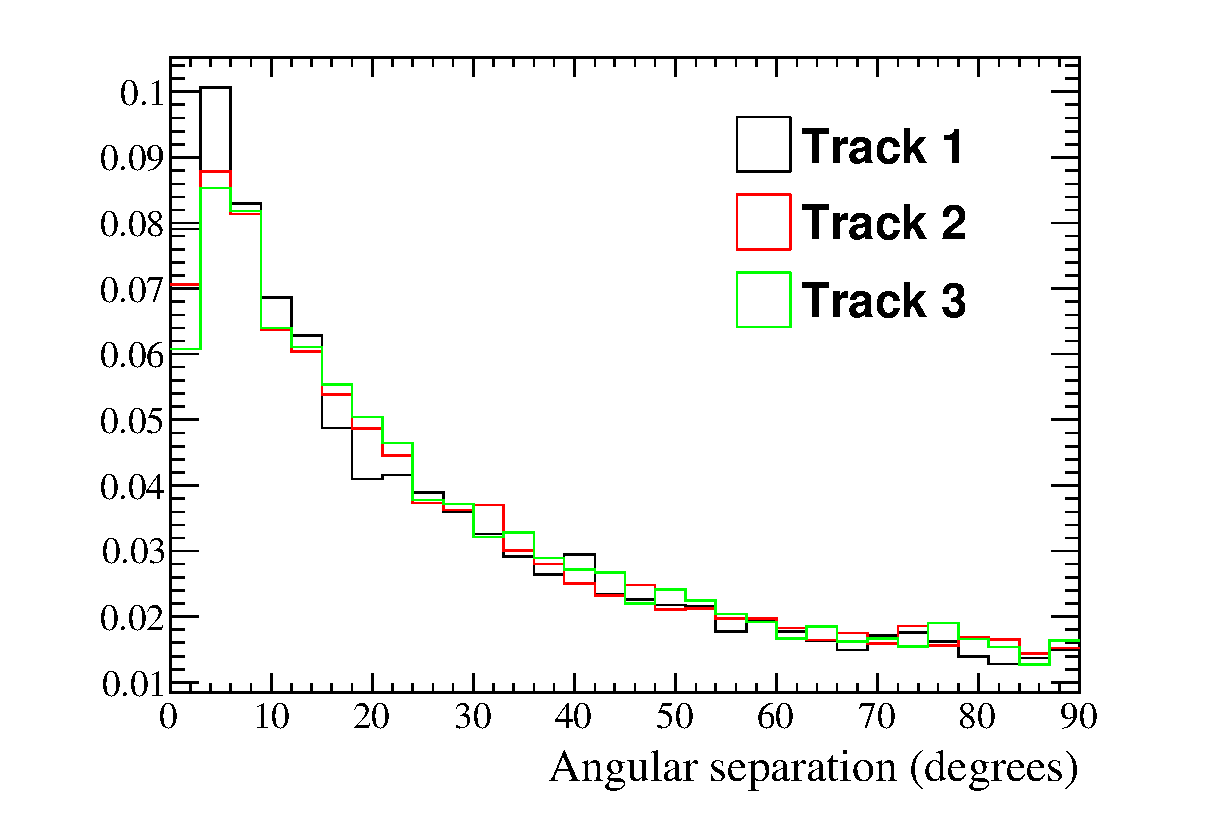
\includegraphics[width=9cm]{images/selection/track_rejection/AngularSeparationWithRejection}\label{fig:AngularSeparationWithRejection}}
  \caption{Angular separation of the reconstructed tracks in an ECal cluster with the beam-simulated particle that created them.  The black, red and green histograms are the tracks that were reconstructed first, second and third respectively.  All histograms are area normalised.}
  \label{fig:TrackRejectionAngularSeparation}
\end{figure}
There are two categories of bad track reconstruction.  The first is where the 3D matching matches two 2D tracks which do not have sufficient information to fully model a 3D track.  Specifically, one of the 2D tracks involved in the matching only uses one ECal layer.  As the 3D track reconstruction requires information from both ECal views, tracks which fall into this category do not supply enough information to reconstruct a good quality track.  The second category is where the 3D matching produces a grossly incorrect match.  The matcher is designed to continually match 2D tracks together until no more 2D tracks are left in the matching pool.  So, there are situations where the last possible match made is in no way suitable.  This situation is easily identified by matched 2D tracks which do not overlap.  For example, one of the 2D tracks uses layers 16, 18 and 20 and the other 2D track uses layers 1 and 3.  By removing these two types of tracks from the cluster, the 90$^\circ$ build up in the angular separation distribution is suppressed, as shown in Fig.~\ref{fig:AngularSeparationWithRejection}.  By removing these categories of tracks, approximately 22$\%$ of tracks are rejected.
\newline
\newline
The final states of a neutrino interaction originate from the same point in space.  So, assuming that the reconstructed tracks represent the final states, the reconstructed tracks should most closely cross at the point of interaction.  As stated above, one of the outputs of the reconstruction are the pairwise crossings of the constituent tracks in the ECal cluster.  Using the above assumptions,  the pairwise crossings should be in close proximity to one another when the reconstructed tracks represent the final states of an interaction.  This idea promotes a relatively simple method of vertex reconstruction: attempt to cluster the pairwise crossings together if the pairwise crossings are in close proximity.  To quantitatively define this proximity, the quality of the pairwise crossing also has to be considered.
\newline 
\newline
As with the 3D tracks, the reconstruction does not perform any quality checks on the pairwise crossings of the tracks.  As the reconstruction will always find a crossing location for a pair of 3D tracks, some of the pairwise crossings will not represent anything physical.  The quality definition chosen is simple: pairwise crossings are defined as bad if the crossing location is far away from either of the tracks it is associated with.  However, the distance definition is not trivial to define and should be closely correlated with the vertex reconstruction method.  For example, a two track vertex would provide very little constraint on the distance which defines a bad crossing, whereas a three track vertex may provide a bad crossing distance constraint which is too strict and destroys the majority two track vertices. 
\newline
\newline
The above discussion promotes two parameters which will govern the vertex reconstruction: the required proximity of two crossings to be clustered together, $d_c$, and the distance of a crossing from its constituents tracks to be classified as bad quality, $d_q$.  To quantify these values, a sample of reconstructed events matched to interactions in the ECals are used which are taken from beam Monte Carlo.  The reconstruction (the pairwise crossing rejection and clustering) is repeatedly run over the sample for different values of the $d_c$ and $d_q$ to find the optimum values.  To define the optimum value, a figure of merit is necessary.  After running the reconstruction for a given $d_c$ and $d_q$, the number vertices are separated into one, two and three track vertices and the true neutrino interactions which created the reconstructed vertices are associated.  A reconstructed vertex is tagged as correctly reconstructed if it contains the same number of reconstructed tracks as the number of charged final states in the associated neutrino interaction.  By defining the number of correctly reconstructed one, two and three track vertices as $N_1$, $N_2$ and $N_3$ respectively, the figure of merit, $\phi^{\textrm{vertices}}$, is
\begin{equation}
  \phi^{\textrm{vertices}} = N_1N_2N_3.
\end{equation}
\begin{figure}
  \centering
  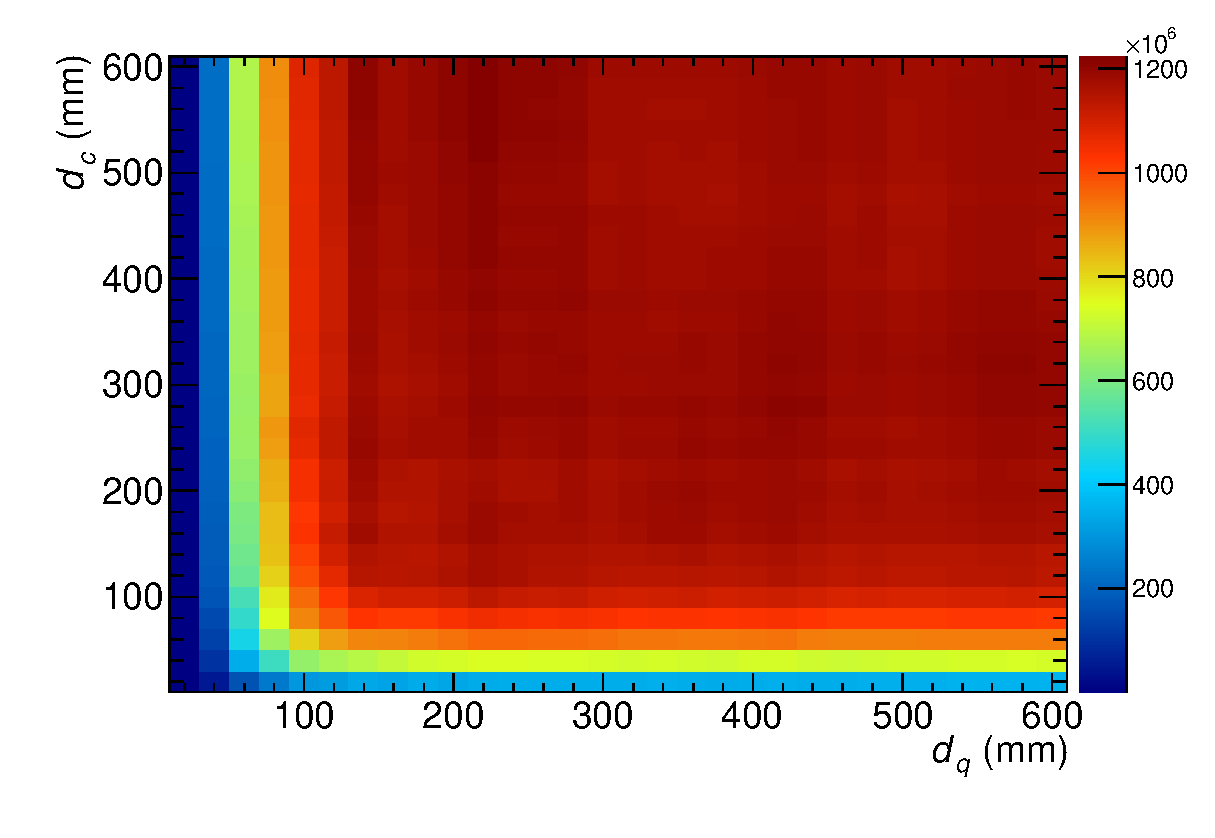
\includegraphics[width=12cm]{images/selection/vertex_recon/FOM_2D}
  \caption{Values of $\phi^{\textrm{vertices}}$ in ($d_q$,$d_c$) space.  The colour corresponds to the magnitude of $\phi^{\textrm{vertices}}$.}
  \label{fig:VertexReconFOM}
\end{figure}
\begin{figure}
  \centering
  \subfloat[$d_q$]{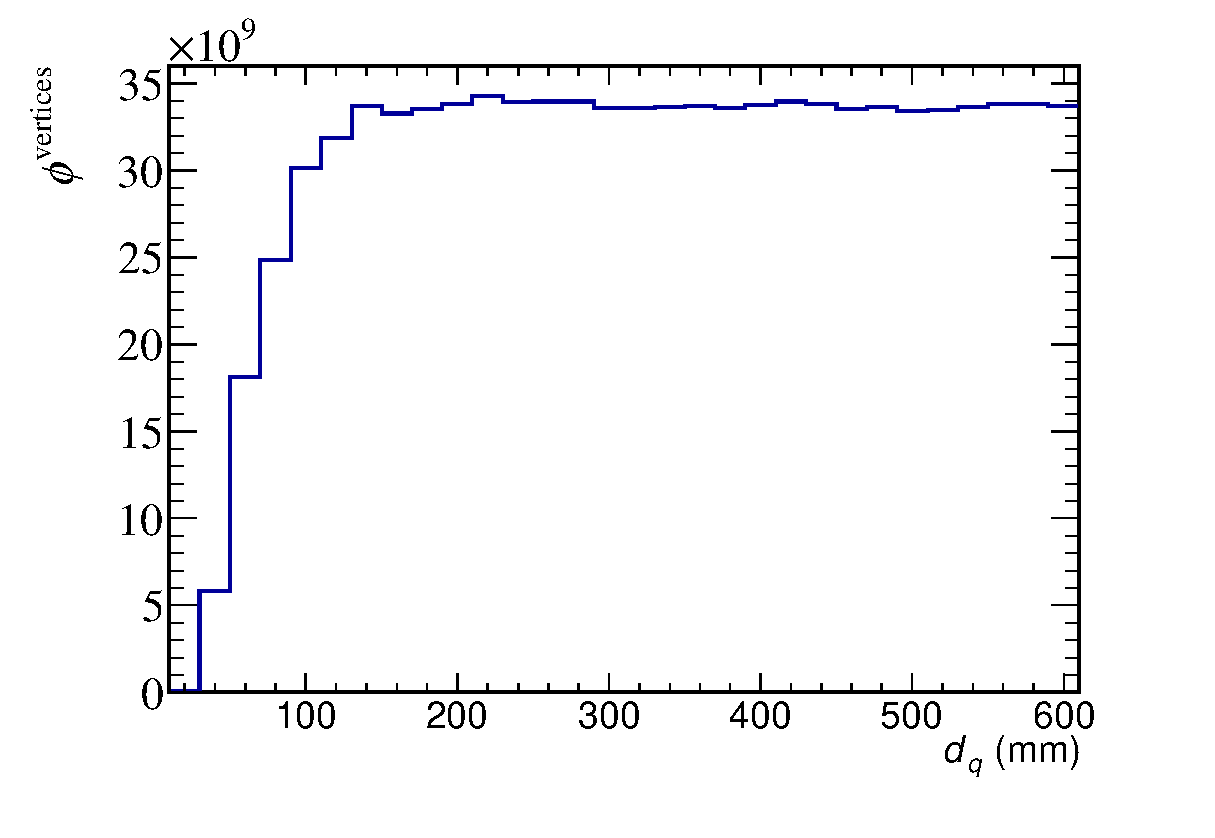
\includegraphics[width=9cm]{images/selection/vertex_recon/dq_marginalize} \label{fig:dqMarginalize}}
  \subfloat[$d_c$]{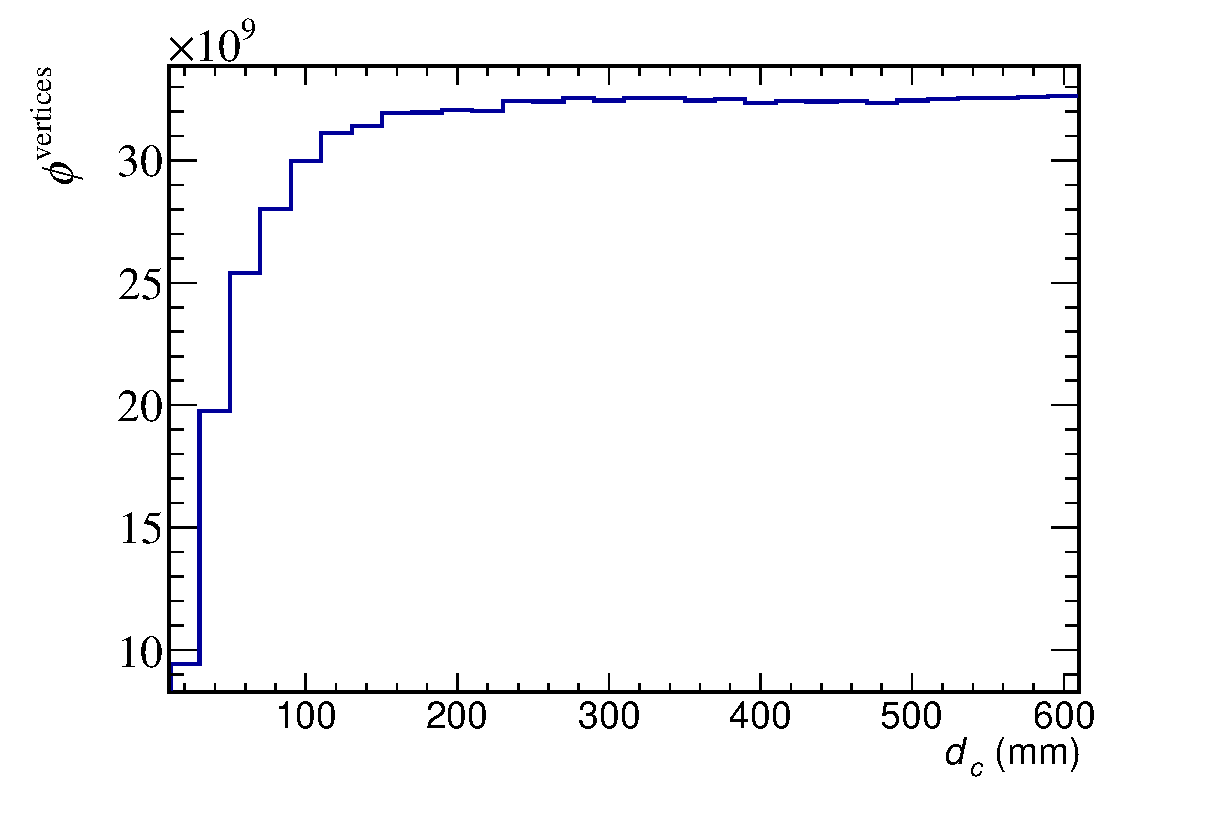
\includegraphics[width=9cm]{images/selection/vertex_recon/dc_marginalize} \label{fig:dcMarginalize}}
  \caption{$\phi^{\textrm{vertices}}$ vs the marginalised vertex reconstruction parameters.}
  \label{fig:VertexReconMarginalizedDistributions}
\end{figure}
By mapping out $\phi^{\textrm{vertices}}$ in ($d_q$,$d_c$) space, information about the preferred values of $d_q$ and $d_c$ can be found.  This space is shown in Fig.~\ref{fig:VertexReconFOM}.  It is clear from Fig.~\ref{fig:VertexReconFOM} that there is no clear maximum, but rather a plateau of  $\phi^{\textrm{vertices}}$ for $d_q$ and $d_c$ greater than 140 mm.  So, marginalised distributions of $d_q$ and $d_c$ can be produced to find where $\phi^{\textrm{vertices}}$ approaches zero which are shown in Fig.~\ref{fig:dqMarginalize} and Fig.~\ref{fig:dcMarginalize} respectively.  The values chosen are shown in table~\ref{table:VertexReconParameters}. 
\begin{table}[t!]
  \begin{tabular}{ c c }
    $\phi_d$ & $\phi_c$ \\ \hline \hline
    $<$ 140 mm & $<$ 200 mm \\
  \end{tabular}
  \caption{Parameters for the vertex reconstruction in the ECal.}
  \label{table:VertexReconParameters}
\end{table}
The reconstruction now assesses the quality of the crossings and then attempts to cluster the good quality crossings together to form vertex candidates.  The final step is to use the constituent tracks of each vertex candidate in a fit to estimate the position of the vertex.  The following method was suggested by X. Lu.  The position of the vertex, $\vec{P}$, is defined such that the sum of the squares of the distance of each track to $\vec{P}$ is minimised.  An example setup of this is shown in Fig.~\ref{fig:VertexVectorDiagram} for three constituent tracks.  By defining the square of the distance of a line, $l_i$, to $\vec{P}$ as $|\vec{r}_i|^2$, the function to minimise is
\begin{figure}[!b]
  \centering
  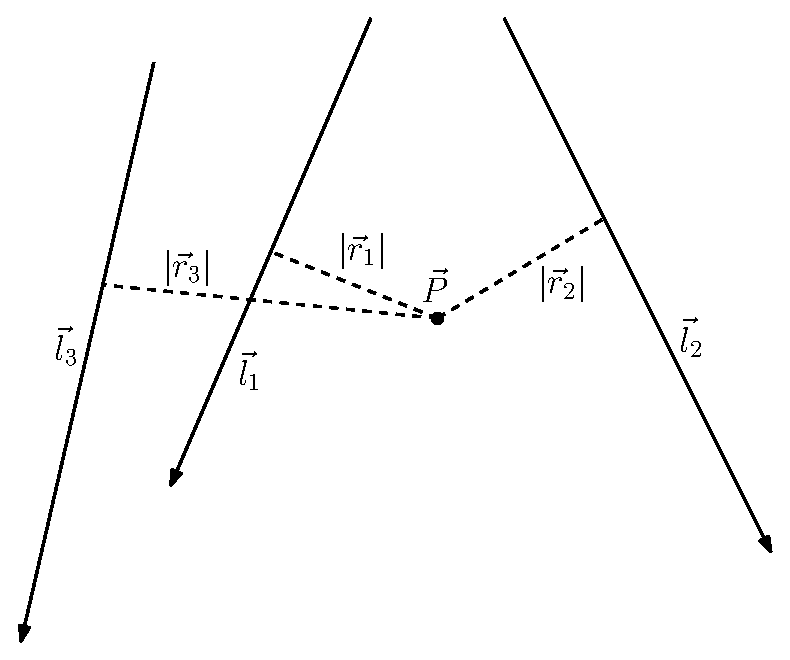
\includegraphics[width=8cm]{images/selection/vertex_recon/vertex_vector_diagram}
  \caption{Example of the vertex position, $\vec{P}$ for three lines: $\vec{l}_1$, $\vec{l}_2$ and $\vec{l}_3$. $|\vec{r}_1|$, $|\vec{r}_2|$ and $|\vec{r}_3|$ are the perpendicular distances of $\vec{l}_1$, $\vec{l}_2$ and $\vec{l}_3$ to $\vec{P}$ respectively.}
  \label{fig:VertexVectorDiagram}
\end{figure}
\begin{equation}
  D = \sum_i |\vec{r}_i|^2.
  \label{eqn:SumOfSquares}
\end{equation}
$\vec{P}$ is then defined as the point in space which satisfies
\begin{equation}
  \frac{\partial D}{\partial x} = \frac{\partial D}{\partial y} = \frac{\partial D}{\partial z} = 0.
  \label{eqn:SumOfSquaresMinCondition}
\end{equation}
The value of $|\vec{r}_i|$ is trivially defined by simple vector properties as 
\begin{equation}
  |\vec{r}_i| = \frac{|(\vec{P} - \vec{a}_i) \cross \vec{v}_i|}{|\vec{v}_i|} = |(\vec{P} - \vec{a}_i) \cross \hat{v}_i|,
  \label{eqn:DistanceOfPointToLine}
\end{equation}
where $\vec{v}_i$ is the direction vector of $\vec{l}_i$ and $\vec{a}_i$ is a point along $\vec{l}_i$.  By defining $\vec{P}$ as
\begin{equation}
  \vec{P} = x\hat{\imath} + y\hat{\jmath} + z\hat{k},
  \label{eqn:PDefinition}
\end{equation}
equation~\ref{eqn:SumOfSquaresMinCondition} can be solved.  The following derivation is only for $\partial D/\partial x$ as the method is identical for $\partial D/\partial x$, $\partial D/\partial y$ and $\partial D/\partial z$.
\begin{eqnarray}
  \frac{\partial D}{\partial x} & = & \sum_i 2\vec{r}_i \cdot \frac{\partial \vec{r}_i}{\partial x} \\
  & = & 2\sum_i \big[(\vec{P} - \vec{a}_i) \cross \hat{v}_i\big] \cdot \big[\hat{\imath} \cross \hat{v}_i\big] \nonumber \\
  & = & 2x \sum_i (\hat{\imath} \cross \hat{v}_i) \cdot ( \hat{\imath} \cross \hat{v}_i) + 2y \sum_i (\hat{\jmath} \cross \hat{v}_i) \cdot ( \hat{\imath} \cross \hat{v}_i) + 2z \sum_i (\hat{k} \cross \hat{v}_i) \cdot ( \hat{\imath} \cross \hat{v}_i) \nonumber \\
  &\qquad & - 2(\vec{a}_i \cross \hat{v}_i) \cdot ( \hat{\imath} \cross \hat{v}_i). \nonumber
  \label{eqn:dDdxDerivation}
\end{eqnarray}
By applying the same steps for $\partial D/\partial y$ and $\partial D/\partial z$, the matrix equation
\begin{equation}
%  \[ \left( \begin{array}{ccc}
%      0 & 0 & 0 \\
%      0 & 0 & 0 \\
%    0 & 0 & 0 \end{array} \right)\]
%  \label{eqn:VertexReconMatrix}
  \begin{pmatrix}
    \displaystyle\sum_i [\hat{\imath} \cross \hat{v}_i] \cdot (\hat{\imath} \cross \hat{v}_i) & \displaystyle\sum_i [\hat{\jmath} \cross \hat{v}_i] \cdot (\hat{\imath} \cross \hat{v}_i) & \displaystyle\sum_i [\hat{k} \cross \hat{v}_i] \cdot (\hat{\imath} \cross \hat{v}_i) \\
    \displaystyle\sum_i [\hat{\imath} \cross \hat{v}_i] \cdot (\hat{\jmath} \cross \hat{v}_i) & \displaystyle\sum_i [\hat{\jmath} \cross \hat{v}_i] \cdot (\hat{\jmath} \cross \hat{v}_i) & \displaystyle\sum_i [\hat{k} \cross \hat{v}_i] \cdot (\hat{\jmath} \cross \hat{v}_i) \\ 
    \displaystyle\sum_i [\hat{\imath} \cross \hat{v}_i] \cdot (\hat{k} \cross \hat{v}_i) & \displaystyle\sum_i [\hat{\jmath} \cross \hat{v}_i] \cdot (\hat{k} \cross \hat{v}_i) & \displaystyle\sum_i [\hat{k} \cross \hat{v}_i] \cdot (\hat{k} \cross \hat{v}_i) 
  \end{pmatrix}
  \begin{pmatrix}
   x \\
   y \\
   z
  \end{pmatrix}
  =
  \begin{pmatrix}
    \displaystyle\sum_i [\vec{a}_i \cross \hat{v}] \cdot (\hat{\imath} \cross \hat{v}) \\
    \displaystyle\sum_i [\vec{a}_i \cross \hat{v}] \cdot (\hat{\jmath} \cross \hat{v}) \\
    \displaystyle\sum_i [\vec{a}_i \cross \hat{v}] \cdot (\hat{k} \cross \hat{v})
  \end{pmatrix}
  \label{eqn:VertexReconMatrix}
\end{equation}
can be built up.  By defining equation~\ref{eqn:VertexReconMatrix} as
\begin{equation}
  \underline{\underline{A}} \vec{P} = \vec{B},
  \label{eqn:VertexReconMatrixSimple}
\end{equation}
where $\underline{\underline{A}}$ is the matrix on the left hand side of equation~\ref{eqn:VertexReconMatrix} and $\vec{B}$ is the vector on the right hand side of equation~\ref{eqn:VertexReconMatrix}.  $\vec{P}$ is finally
\begin{equation}
  \vec{P} = \underline{\underline{A}}^{-1} \vec{B}.
  \label{eqn:VertexReconMatrixSolution}
\end{equation}
While the inversion of $\underline{\underline{A}}$ is in principle analytically solvable, it was decided that the inversion would be handled numerically.  So, to find $\vec{P}$, the vertex reconstruction builds $\underline{\underline{A}}^{-1}$ (by building and inverting $\underline{\underline{A}})$ and $\vec{B}$ and then applies equation~\ref{eqn:VertexReconMatrixSolution}.
\newline
\newline
By applying the steps outlined above to every reconstructed ECal cluster, a set of candidate vertices are formed.  As the enhanced reconstruction is only capable of reconstructing straight tracks, bending trajectories tend to be reconstructed as two or more tracks.  The crossings associated with such tracks can, and do, pass the vertex reconstruction criteria defined in table~\ref{table:VertexReconParameters}.  An extreme example of this topology is shown in Fig.~\ref{fig:TrackMergingEventDisplay} in which a curving $\mu^-$ is reconstructed as four tracks.  So, the final step of the reconstruction is to attempt to merge tracks to model the curving trajectory topology.  Firstly, the reconstructed crossings associated with a clean curving trajectory should pass the pairwise crossing quality cut but should be sufficiently far away from any other crossings that it is not clustered during the vertex clustering stage.  Therefore, track merging candidates can be initially identified by searching for reconstructed vertices with exactly two track constituents.  As an example, all three of the crossings shown in Fig.~\ref{fig:TrackMergingEventDisplay} are correctly identified by this check.  The two constituent tracks of the identified vertex will form the merged track, so the reconstruction checks the shape that the merged track would make against a set of conditions to decide if the merging should be performed. 
\begin{figure}
  \centering
  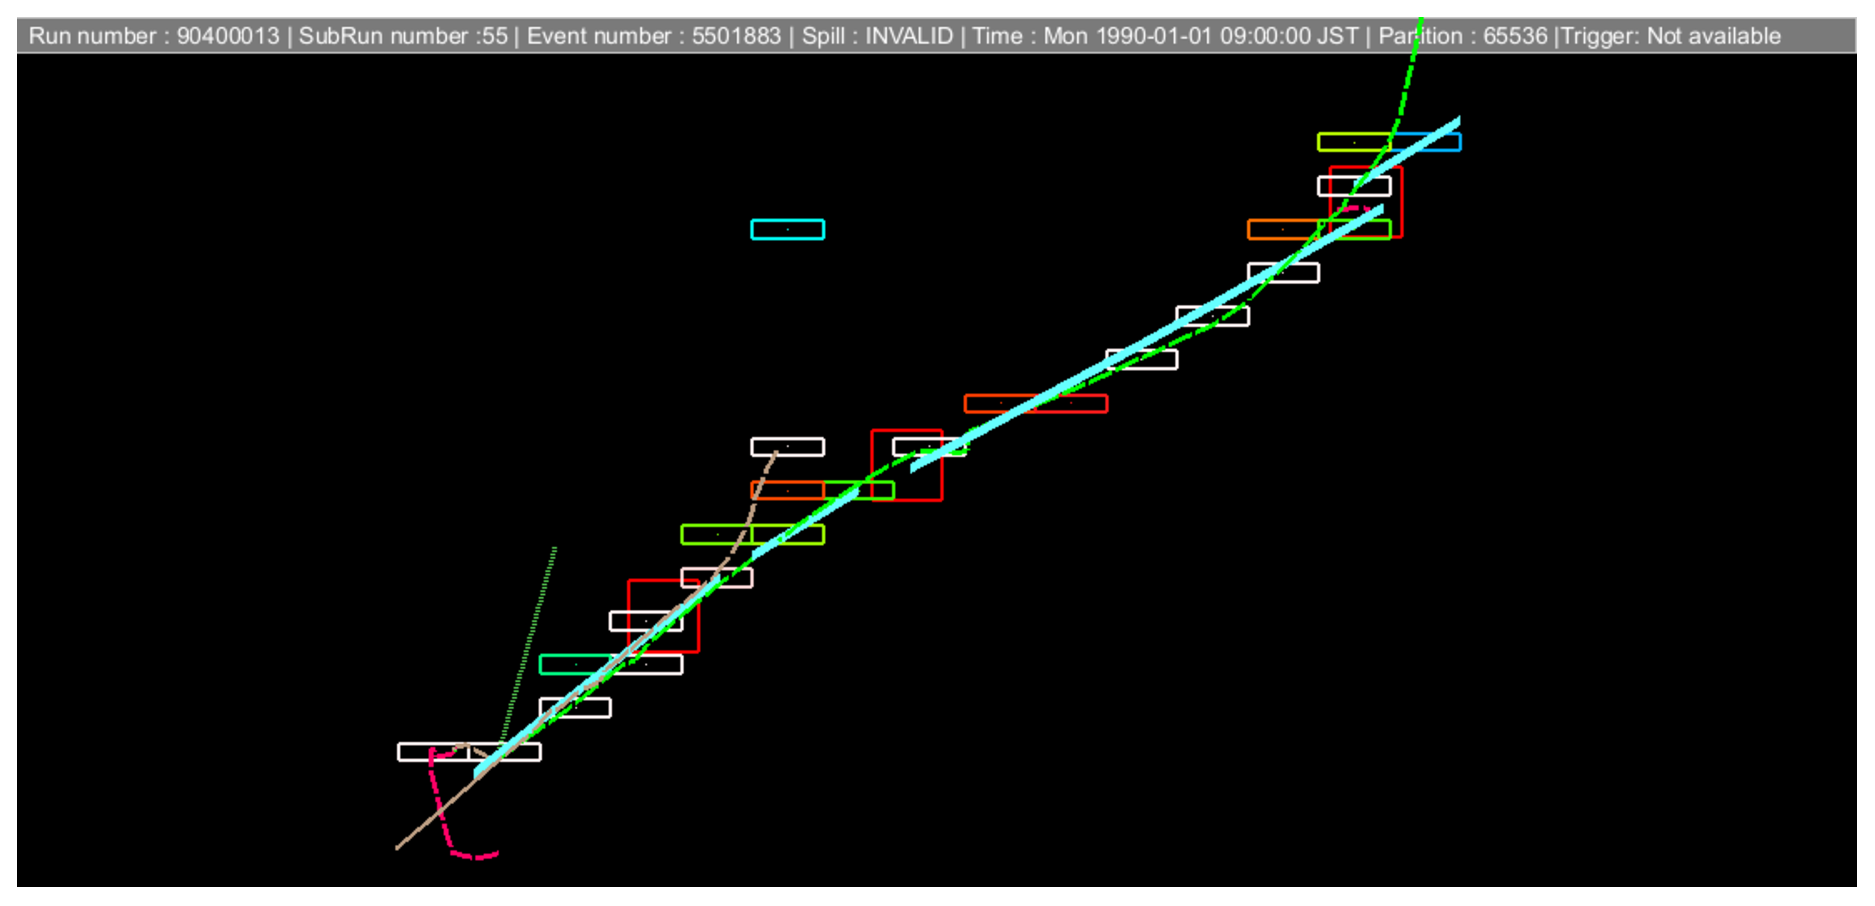
\includegraphics[width=12cm]{images/selection/vertex_recon/track_merging_event_display.eps}
  \caption{Example event display showing a set of track merging candidates.  The final state $\mu^-$ (in green) curves in a complicated way and is reconstructed as four tracks (in light blue).  The pairwise crossings of the reconstructed tracks are the red squares.  The muon is produced by a charged current interaction in the top left barrel ECal producing two $\pi^+$ (in brown) and the curving $\mu^-$. }
  \label{fig:TrackMergingEventDisplay}
\end{figure}
To identify and tune the conditions for merging tracks, two metrics are used.  The first metric is used for identification of the merging conditions and uses the truth information provided by the Geant4 simulation.  For every two track vertex that was formed by the vertex clustering, the simulated particle that produced each of the two constituent tracks was checked.  If the same simulated particle is matched to both tracks, then the merging candidate is tagged as a correct match, otherwise it is tagged as an incorrect match.  The second metric is used for tuning the identified merging conditions.  As part of this analysis is a search for neutrino interactions using vertex-based reconstruction, there will be an expected loss of signal by track merging which must be minimised.  So, the track merging condition tuning should be based on ECal signal interactions.  As described above, the only tracks that are proposed as merging candidates are those which are constituents of a two track vertex.  So, the track merging tuning attempts to separate signal and background events which are reconstructed as a vertex with two track constituents.  It is preferable that the merging chooses quality over quantity so the tuning figure of merit is defined as 
\begin{equation}
  \phi^{\textrm{merge}} = \epsilon \eta^2
  \label{eqn:TrackMergingTuningMetric}
\end{equation}
where $\epsilon$ is the efficiency of the track merging to keep signal events reconstructed as two track vertices and $\eta$ is the purity of the events that remain as two track vertices after merging has taken place.
\newline
\newline
The first merging condition identified is the cosine of the opening angle, $\cos\theta$, subtended by the two constituent tracks bounded between 0 and 1 which is shown in Fig.~\ref{fig:TrackMergingConditionCosTheta}.  The opening angle is clearly a powerful discriminator.  The distribution for incorrect matches is very flat across the full angular range whereas there is a clear build up of correct matches as $\cos\theta \rightarrow 1$.
\begin{figure}[!t]
  \centering
  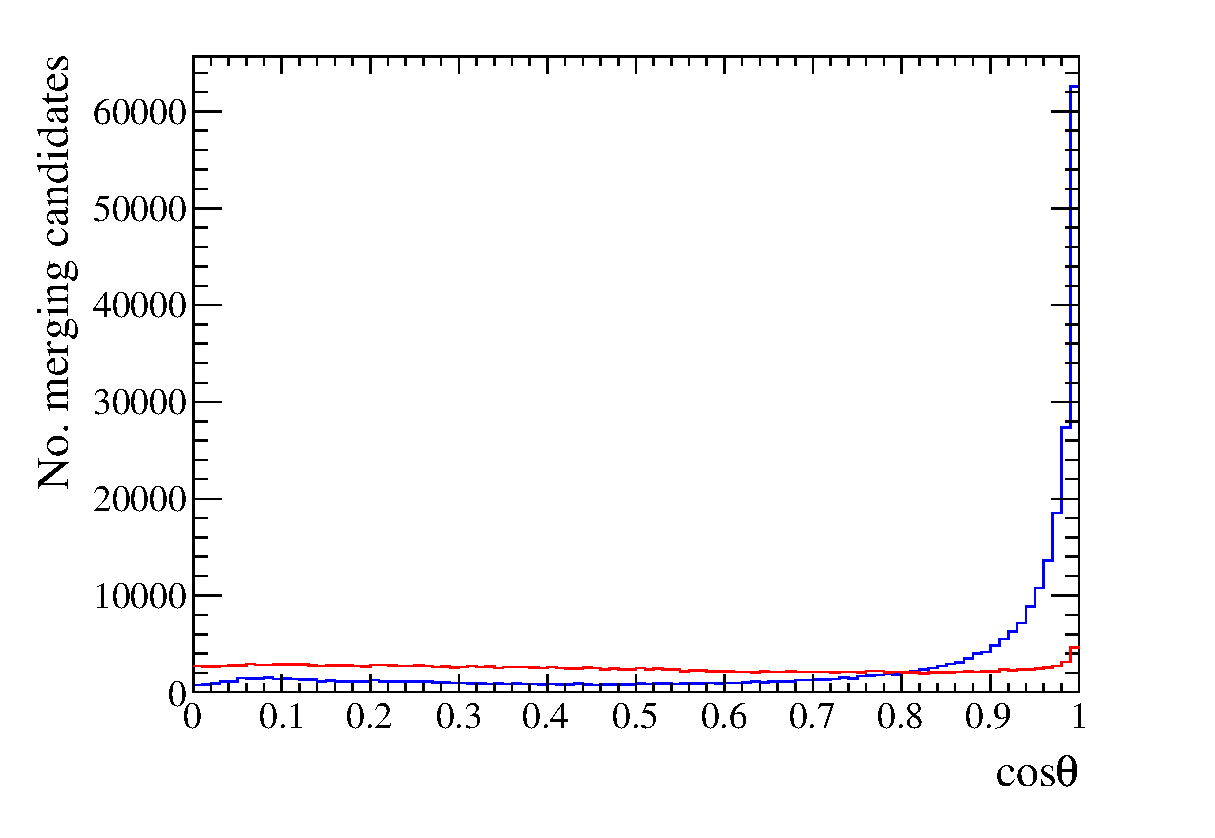
\includegraphics[width=10cm]{images/selection/vertex_recon/merging_candidates_cos_theta}
  \caption{The cosine of the angle subtended by the merging candidates, bounded between 0 and 1. The correct matches and incorrect matches are the blue and red histograms respectively.}
  \label{fig:TrackMergingConditionCosTheta}
\end{figure}
\newline
\newline
The second merging condition identified, called 'distance ratio', measures the ratio of the distance between the two constituent tracks' closest points, $d^{\textrm{small}}$ to the distance between their furthest points, $d^{\textrm{large}}$.  An example of how $d^{\textrm{small}}$ and $d^{\textrm{large}}$ are calculated is shown in Fig.~\ref{fig:DistanceRatioEventDisplay}.    
\begin{figure}[!b]
  \centering
  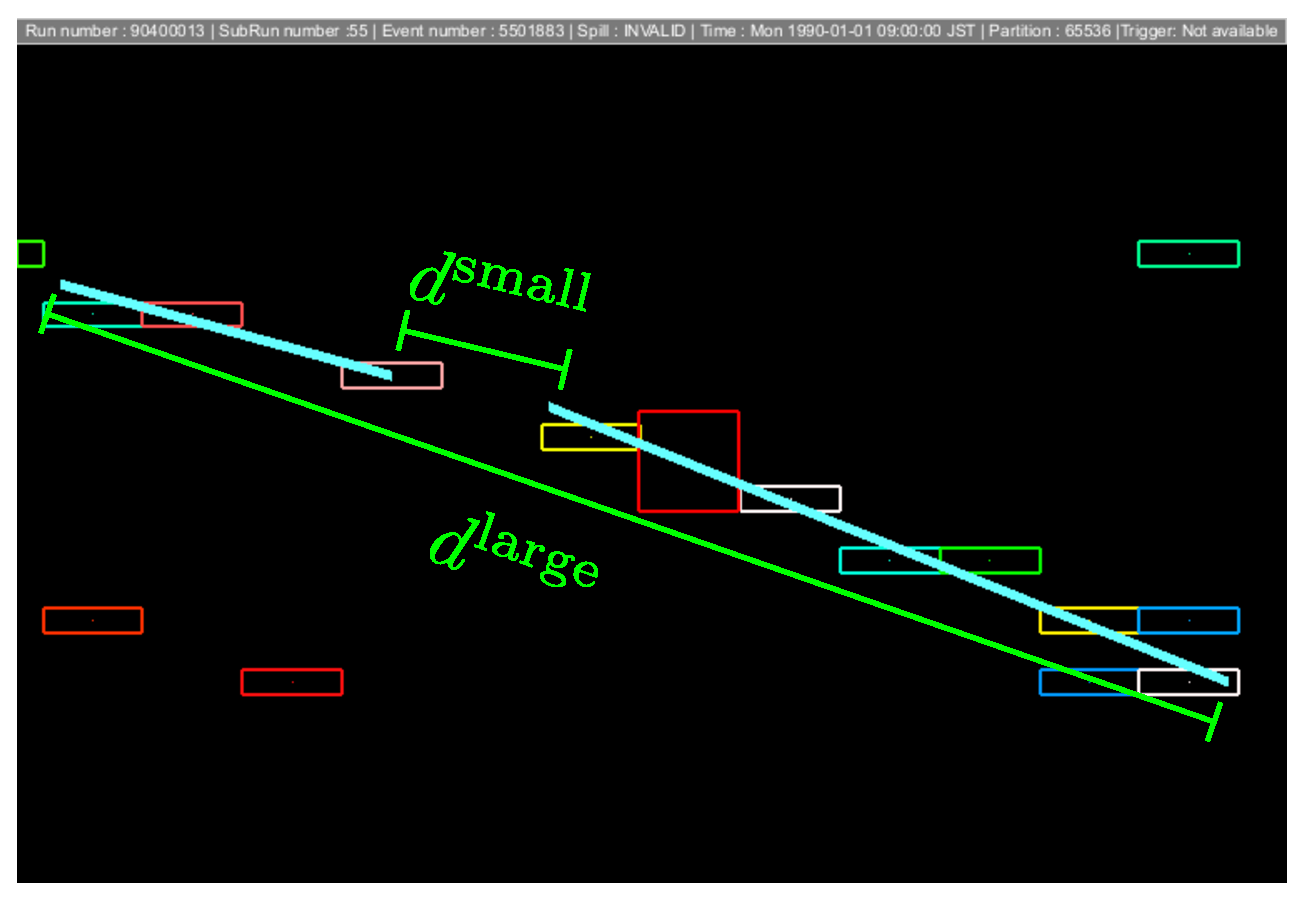
\includegraphics[width=10cm]{images/selection/vertex_recon/distance_ratio_event_display}
  \caption{Example event display showing how the parameters of the distance ratio are calculated.  The distance ratio is defined as $d^{\textrm{small}}/d^{\textrm{large}}$.  The blue lines are the two reconstructed tracks which form the merging candidate and the red square is the crossing location of those tracks.}
  \label{fig:DistanceRatioEventDisplay}
\end{figure}
The distance ratio distribution is shown Fig.~\ref{fig:TrackMergingConditionDistanceRatioNoCut}.  While it may seem that there is very little discrimination power present in the distance ratio distribution, there is an underlying dependency between the distance ratio and the opening angle subtended by the constituent tracks, which has already been identified as a merging condition.
\begin{figure}
  \centering
  \subfloat[No cuts applied.]{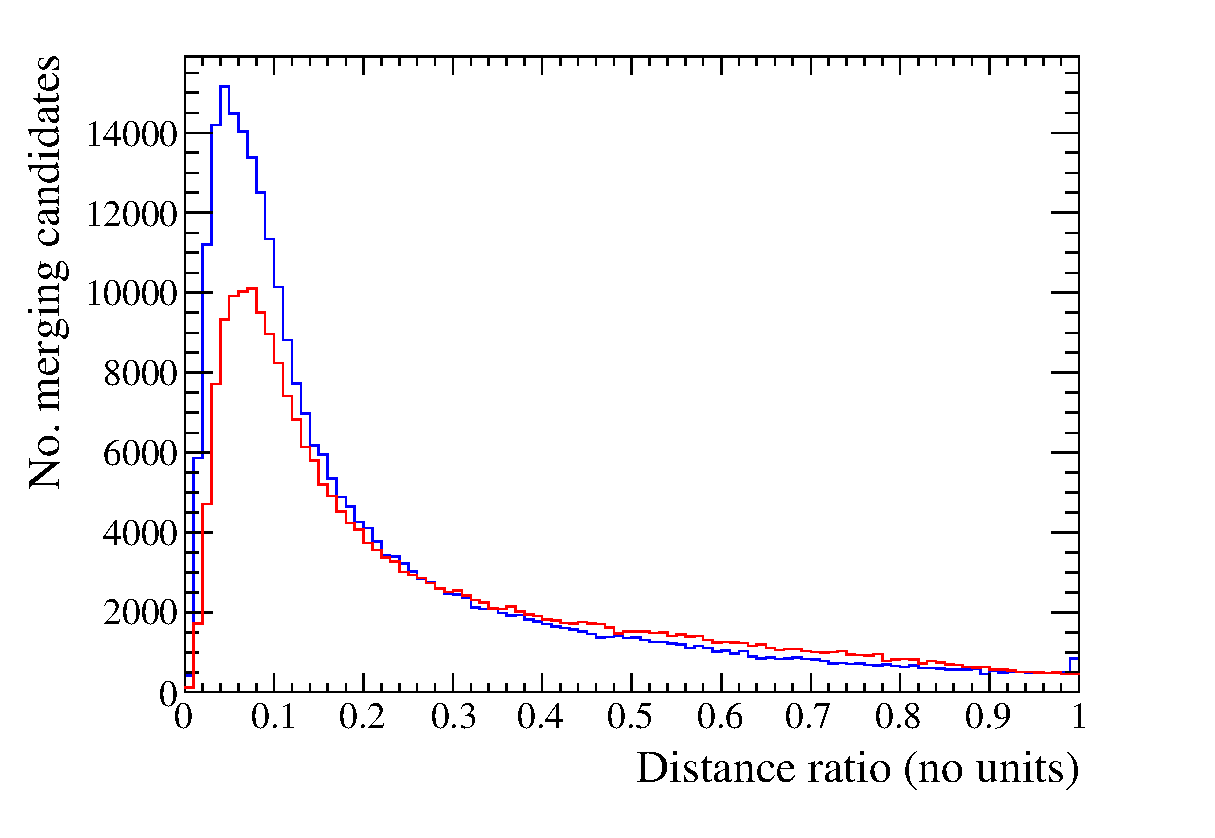
\includegraphics[width=9cm]{images/selection/vertex_recon/merging_candidates_distance_ratio.eps} \label{fig:TrackMergingConditionDistanceRatioNoCut}}
  \subfloat[For $\cos\theta > 0.8$.]{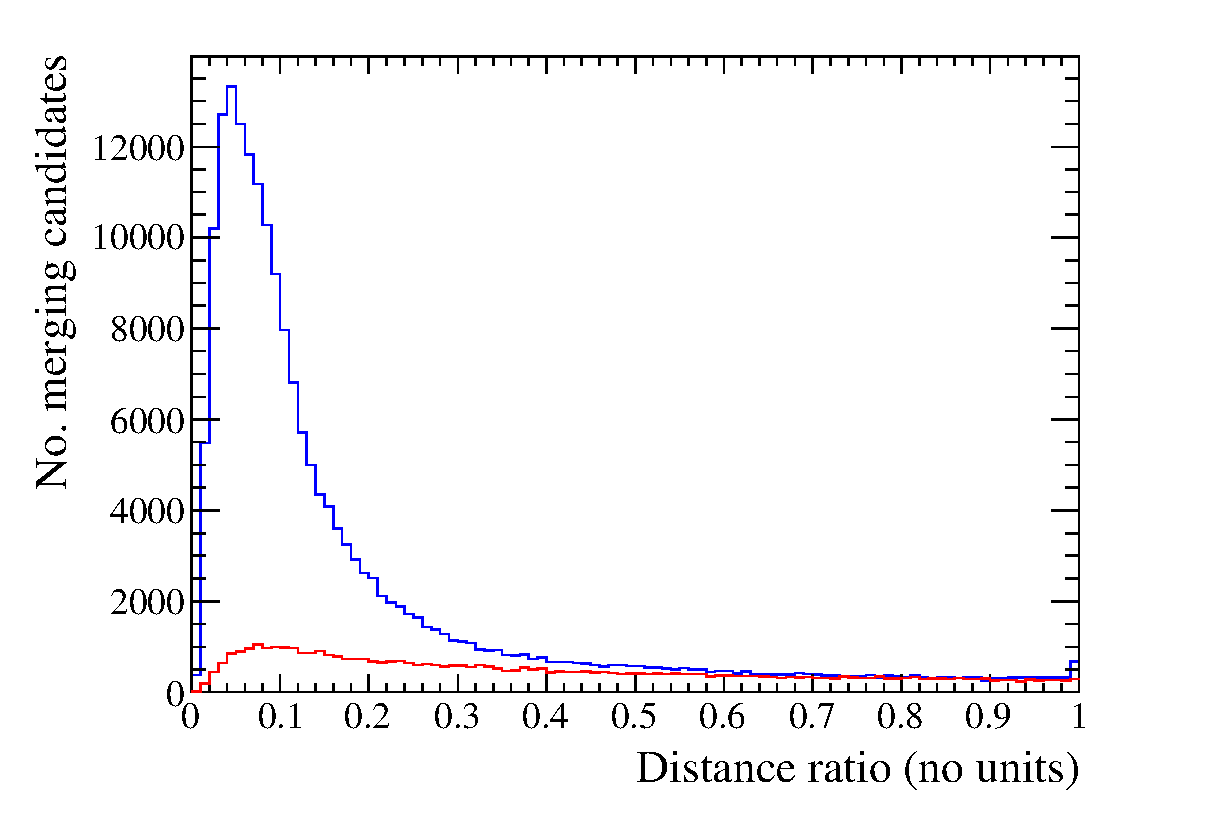
\includegraphics[width=9cm]{images/selection/vertex_recon/merging_candidates_distance_ratio_CosThetaGuessCut.eps} \label{fig:TrackMergingConditionDistanceRatioGuessCutCosTheta}}
  \caption{The distance ratio of the merging candidates.  The correct and incorrect matches are the blue and red histograms respectively.}
  \label{fig:TrackMergingConditionDistanceRatio}
\end{figure}
To illustrate this dependency, two distributions are shown in Fig.~\ref{fig:TrackMergingConditionDistanceRatioVsCosTheta} which both show the distance ratio vs the cosine of the opening angle.  Fig.~\ref{fig:TrackMergingConditionDistanceRatioVsCosThetaCorrectMatch} only shows the correct matches and Fig.~\ref{fig:TrackMergingConditionDistanceRatioVsCosThetaIncorrectMatch} only shows the incorrect matches.  While it is true that there is a pileup of both correct matches and incorrect matches for low values of the distance ratio, the opening angle separates the two categories out.  Specifically, the correct matches pileup occurs as $\cos\theta \rightarrow 1$ and the incorrect matches pileup occurs as $\cos\theta \rightarrow 0$.  To further illustrate this point, a new distance ratio distribution is shown in Fig.~\ref{fig:TrackMergingConditionDistanceRatioGuessCutCosTheta}, but with a $\cos\theta > 0.8$ guess cut applied.  Comparing the distributions shown in Fig.~\ref{fig:TrackMergingConditionDistanceRatioNoCut} and Fig.~\ref{fig:TrackMergingConditionDistanceRatioGuessCutCosTheta}, the effect of the $\cos\theta$ cut can clearly be seen.  The original pileup of incorrect matches seen in Fig.~\ref{fig:TrackMergingConditionDistanceRatioNoCut} is now gone, leaving an essentially flat incorrect matches distribution in Fig.~\ref{fig:TrackMergingConditionDistanceRatioGuessCutCosTheta} while leaving the correct matches structure intact.  
\begin{figure}[b!]
  \centering
  \subfloat[Correct matches only]{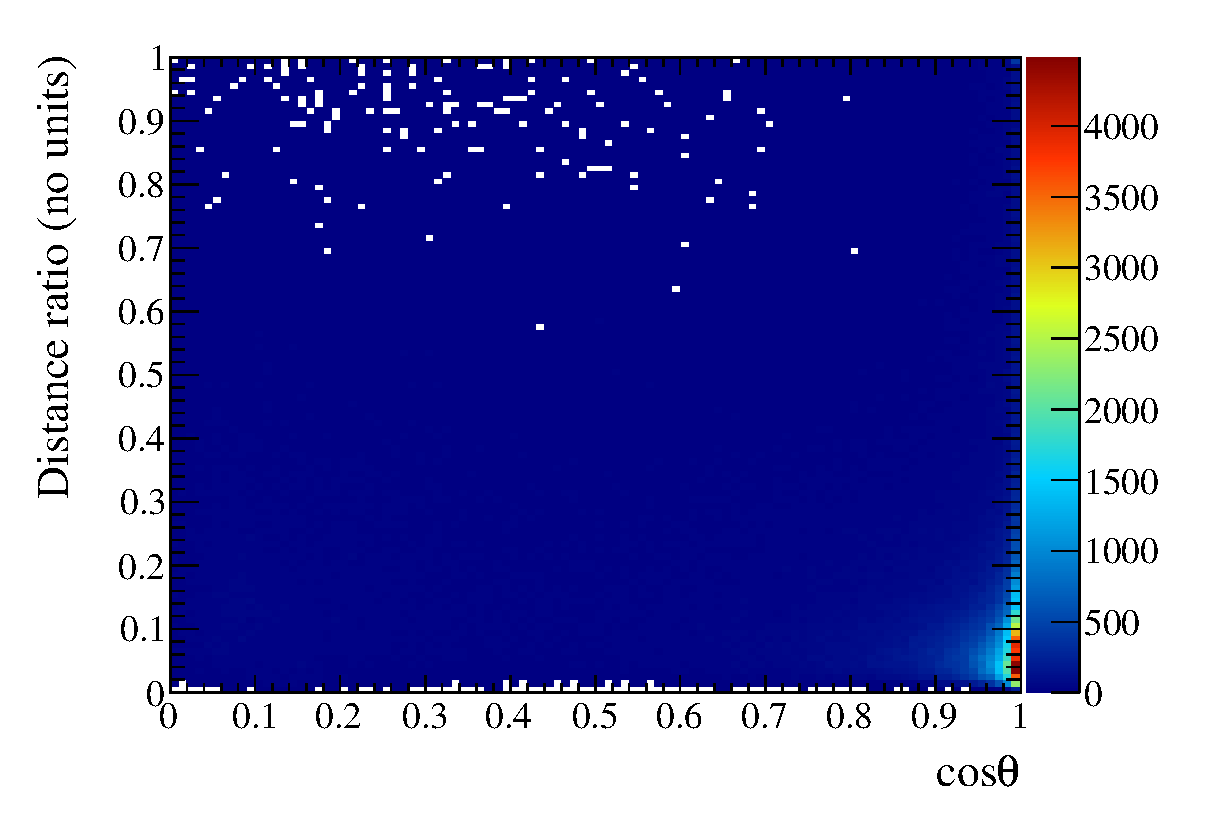
\includegraphics[width=9cm]{images/selection/vertex_recon/correct_merging_candidates_distance_ratio_vs_cos_theta.eps} \label{fig:TrackMergingConditionDistanceRatioVsCosThetaCorrectMatch}}
  \subfloat[Incorrect matches only]{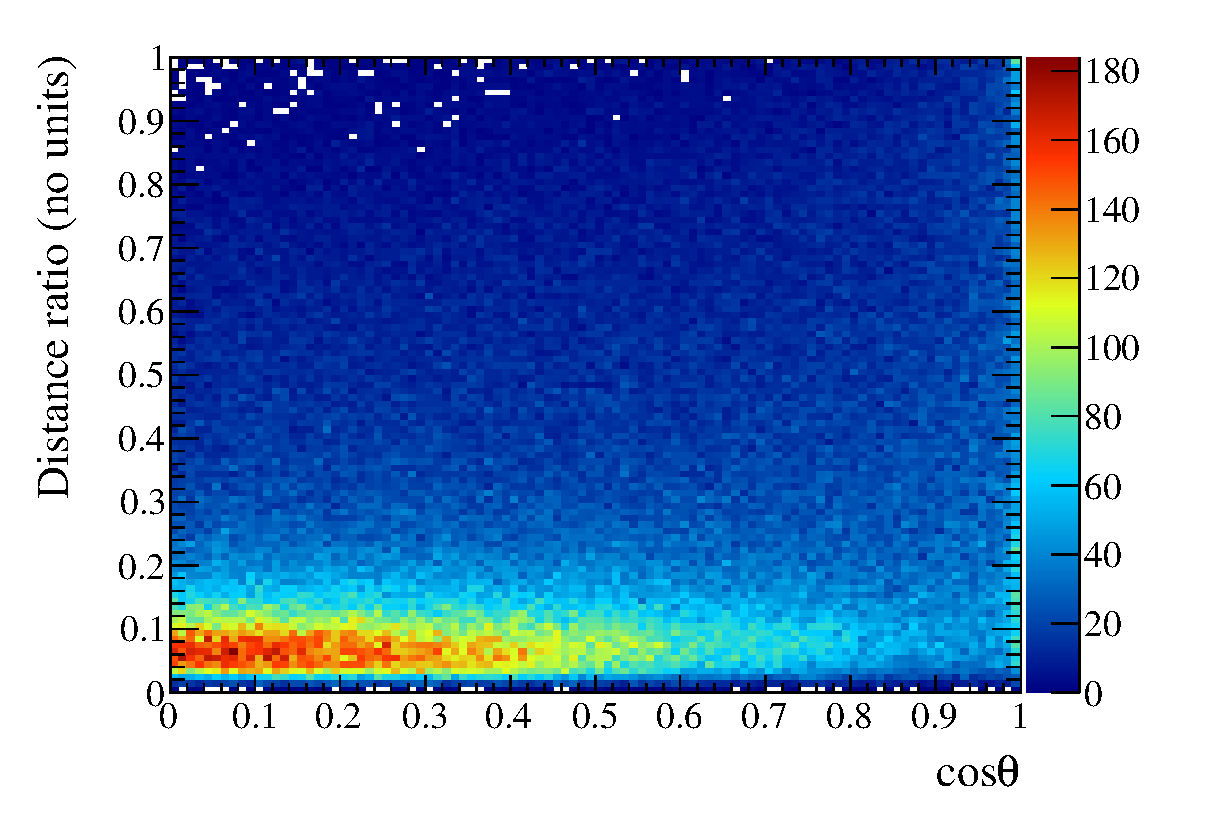
\includegraphics[width=9cm]{images/selection/vertex_recon/incorrect_merging_candidates_distance_ratio_vs_cos_theta.eps} \label{fig:TrackMergingConditionDistanceRatioVsCosThetaIncorrectMatch}}
  \caption{The distance ratio vs the cosine of the opening angle for track merging candidates.}
  \label{fig:TrackMergingConditionDistanceRatioVsCosTheta}
\end{figure}
\newline
\newline
By utilising both the distance ratio and $\cos\theta$ simultaneously, a better degree of separation can be found.  However care must be taken when tuning the distance ratio and $\cos\theta$ cuts to ensure optimal separation of signal and background is achieved.  It is clear from Fig.~\ref{fig:TrackMergingConditionCosTheta} and Fig.~\ref{fig:TrackMergingConditionDistanceRatioGuessCutCosTheta} that the correct matches pileup for low values of the distance ratio and high values of $\cos\theta$.  So events should only be tagged for merging when they have a distance ratio value lower than some threshold and a $\cos\theta$ value higher than some other threshold. To find these cut values, the track merging reconstruction was run multiple times, using different values of the thresholds for each run.  To take the dependency shown in Fig.~\ref{fig:TrackMergingConditionDistanceRatioVsCosTheta} into account, a square grid search in distance ratio and $\cos\theta$ space was used to find optimum cut values.  The tuning metric, as described in equation~\ref{eqn:TrackMergingTuningMetric}, was used to find the optimum cut values.
\begin{figure}[!b]
  \centering
  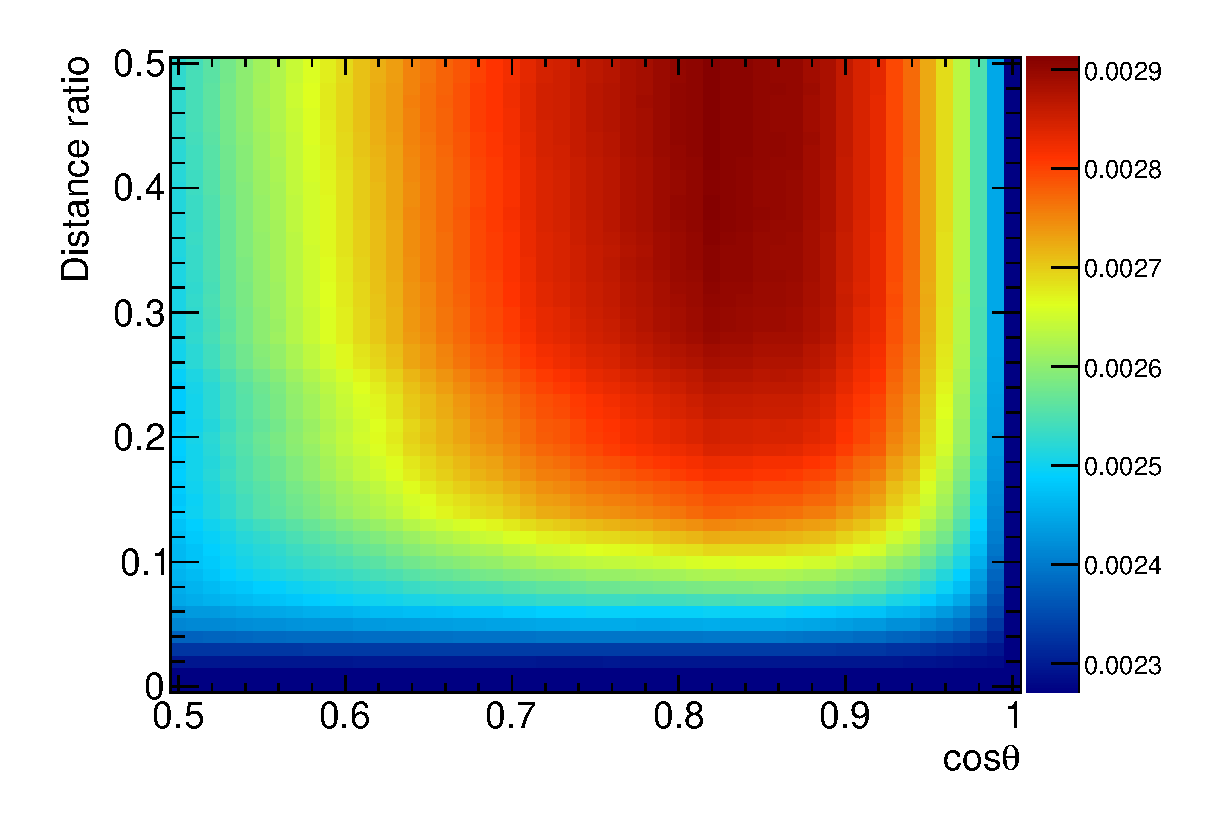
\includegraphics[width=10cm]{images/selection/vertex_recon/TrackMergingTuningFOM}
  \caption{Values of the tuning metric, as described in equation~\ref{eqn:TrackMergingTuningMetric}, in distance ratio cut vs $\cos\theta$ cut space.}
  \label{fig:TrackMergingTuningFOM}
\end{figure}
The tuning metric values in distance ratio cut vs $\cos\theta$ cut space are shown in Fig.~\ref{fig:TrackMergingTuningFOM}.  As was found in the tuning of the vertex clustering parameters, there is no clear maximum value of the tuning metric, but rather a plateau.  So, as was done in the vertex clustering tuning, marginalised distributions of tuning metric in distance ratio cut space and $\cos\theta$ cut space can be produced to find the optimum cut values. 
\begin{figure}
  \centering
  \subfloat[$\cos \theta$]{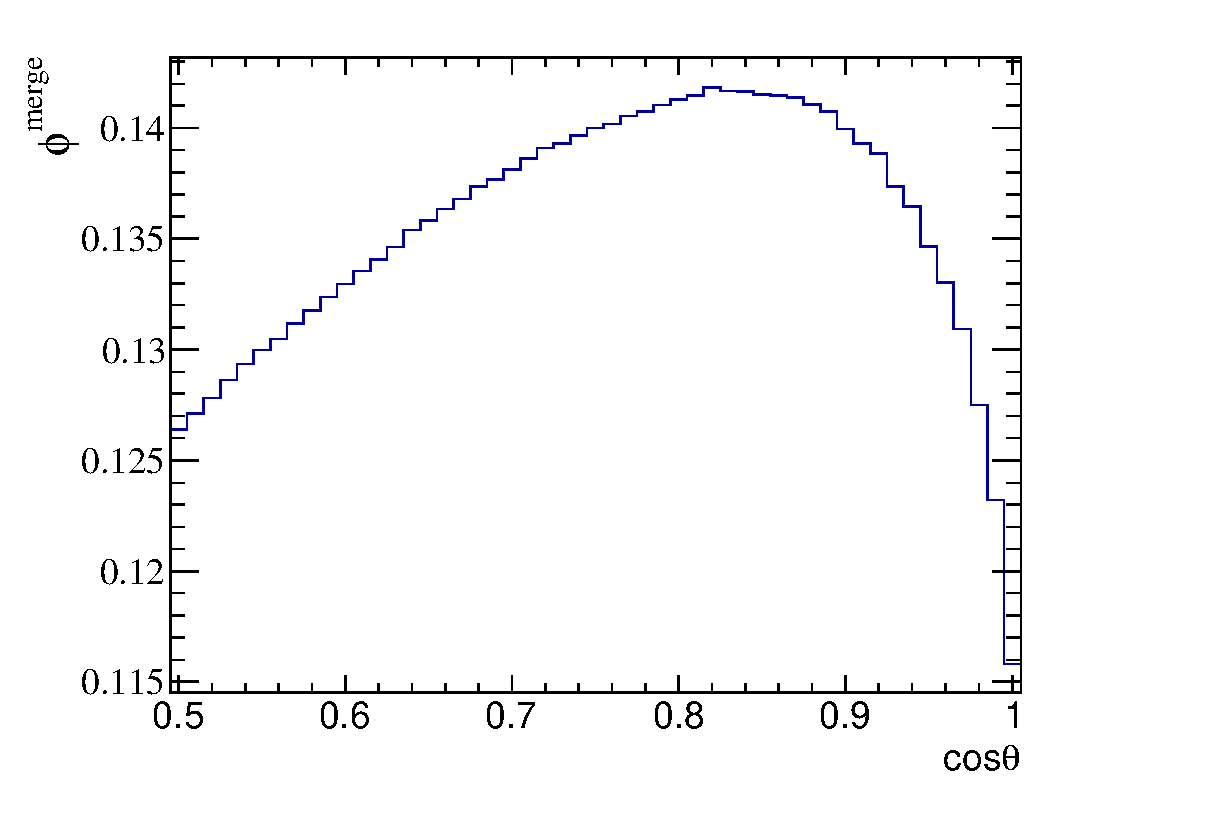
\includegraphics[width=9cm]{images/selection/vertex_recon/TrackMergingMarginalisedCosThetaFOM.eps} \label{fig:TrackMergingCosThetaMarginalize}}
  \subfloat[Distance ratio]{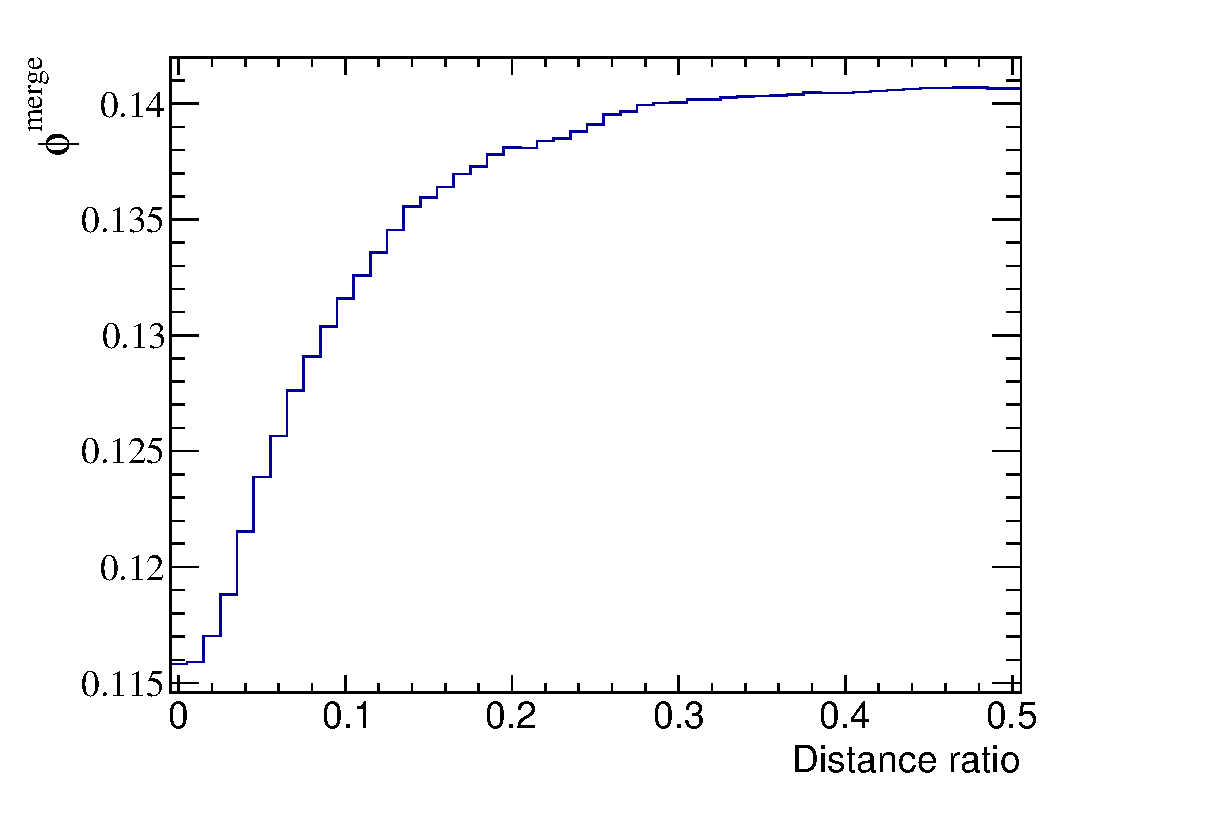
\includegraphics[width=9cm]{images/selection/vertex_recon/TrackMergingMarginalisedDistanceRatioFOM.eps} \label{fig:TrackMergingDistanceRatioMarginalize}}
  \caption{$\phi^{\textrm{merge}}$ vs the track merging conditions.}
  \label{fig:TrackMergingMarginalizedDistributions}
\end{figure}
The marginalised distributions for $\cos\theta$ and the distance ratio cuts are shown in Fig.~\ref{fig:TrackMergingCosThetaMarginalize} and Fig.~\ref{fig:TrackMergingDistanceRatioMarginalize} respectively.  In the case of the $\cos\theta$ cut there is a clearly preferred value, merging candidates should only be merged if $\cos\theta > 0.82$.  In the case of the distance ratio cut distribution, there is less of a clear maximum.  As the reconstruction is striving for quality over quantity, the cut value should be fairly close to the drop in $\phi^{\textrm{merge}}$.  It was decided that merging candidates should only be merged if the distance ratio is less than 0.32.
\newline
\newline
While the $\cos\theta$ condition is clearly a powerful discriminator, there is a topology degeneracy which $\cos\theta$ is not capable of separating, which is shown in Fig.~\ref{fig:TrackMergingCosThetaDegeneracySchematic}.  The diagram on the left of Fig.~\ref{fig:TrackMergingCosThetaDegeneracySchematic} is a representation of a signal event which is reconstructed as two tracks, whereas the diagram on the right of Fig.~\ref{fig:TrackMergingCosThetaDegeneracySchematic} represents a curving trajectory reconstructed as two tracks.  Importantly, the same opening angle is measured for both situations which is small enough that both topologies pass the $\cos\theta$ track merging condition.  To rectify this, an extra sanity check is needed when considering merging candidates.  So, the final merging condition identified, called 'swing', measures the rotation of one track relative to the other.  Specifically, the swing is the ratio of the longest track length, $l^{\textrm{long}}$, to $d^{\textrm{large}}$ (the same $d^{\textrm{large}}$ that was used in the distance ratio calculation).  An example of how these values are calculated is shown in Fig.~\ref{fig:TrackMergingEventDisplaySwing}.  Provided that the opening angle of a merging candidate is not near 90$^\circ$, the swing should be less than one for the topology on the left of Fig.~\ref{fig:TrackMergingCosThetaDegeneracySchematic} and should be greater than one for the topology on the right of Fig.~\ref{fig:TrackMergingCosThetaDegeneracySchematic}.  The separation power of the swing parameter is shown in Fig.~\ref{fig:TrackMergingSwing}.  After applying the merging conditions discussed above, the swing parameter becomes bi-modal as shown in Fig.~\ref{fig:TrackMergingSwingOtherCutsApplied}.  The swing parameter is introduced purely as an extra sanity cut which is physically motivated and requires no tuning.  So, merging candidates are only merged if the measured swing is less than one.
\begin{figure}
  \centering
  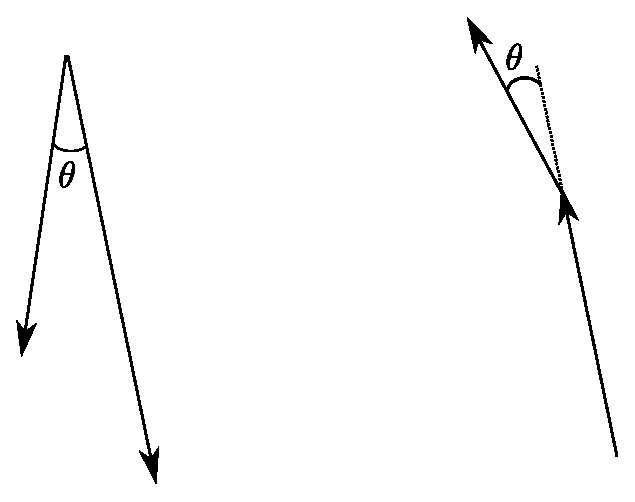
\includegraphics[width=6cm]{images/selection/vertex_recon/TrackMergingCosThetaDegeneracySchematic.eps}
  \caption{Schematic showing the degeneracy of two merging candidate topologies which would pass the $\cos\theta$ cut.  The arrows represent reconstructed tracks and $\theta$ is the opening angle measured between the tracks.}
  \label{fig:TrackMergingCosThetaDegeneracySchematic}
\end{figure}
\begin{figure}
  \centering
  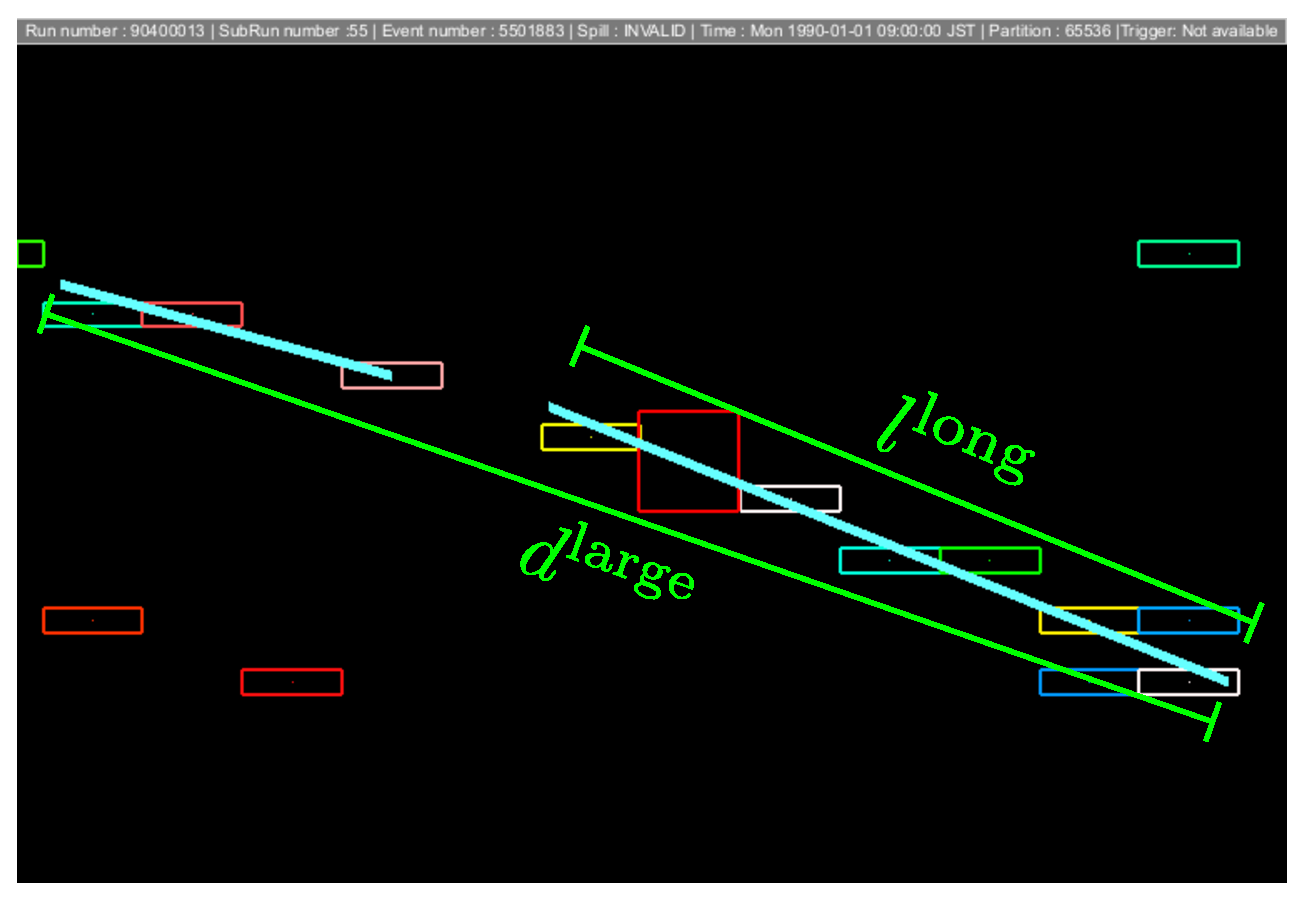
\includegraphics[width=7cm]{images/selection/vertex_recon/track_merging_event_display_swing.eps}
  \caption{Example event display showing how the inputs to the swing parameter are calculated.  Swing is defined as $l^{\textrm{long}}/d^{\textrm{large}}$.  The blue lines are the two reconstructed tracks which form the merging candidate and the red square is the crossing location of those tracks.}
  \label{fig:TrackMergingEventDisplaySwing}
\end{figure}
\begin{figure}
  \centering
  \subfloat[No cuts applied.]{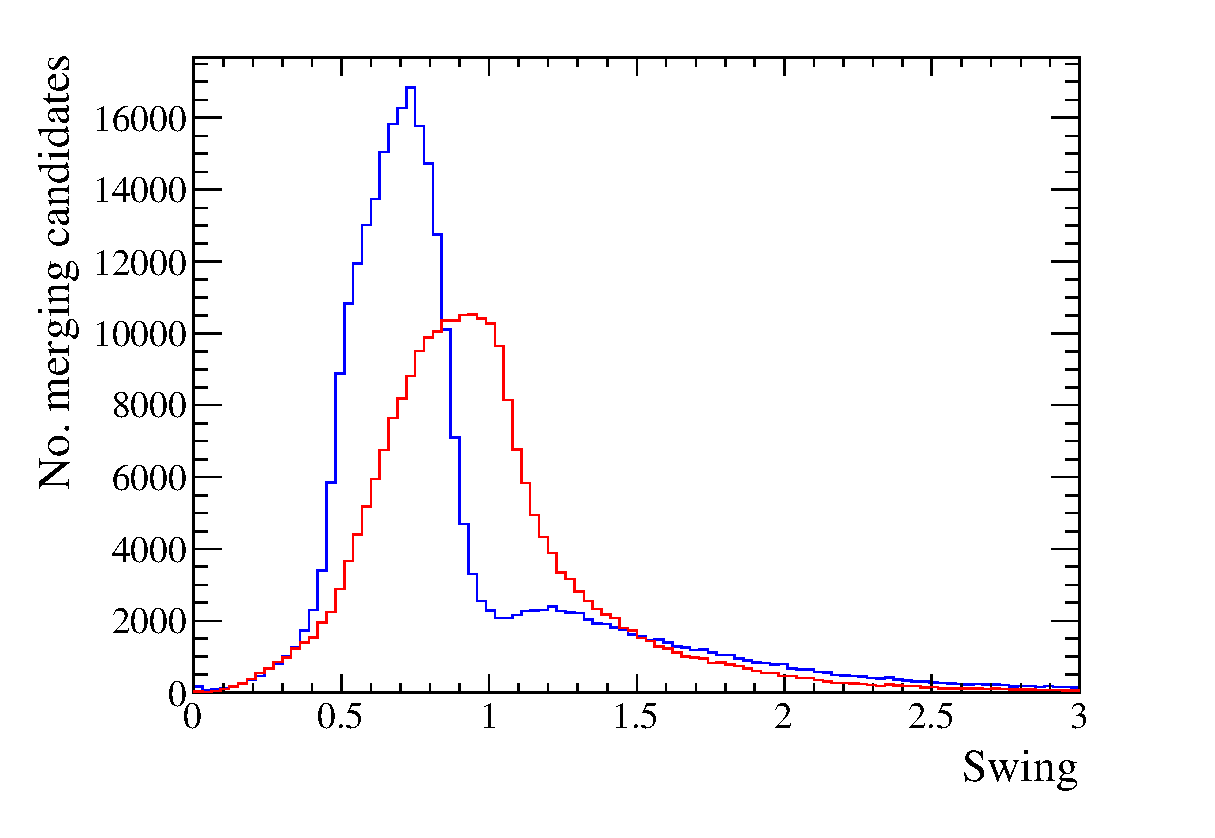
\includegraphics[width=7cm]{images/selection/vertex_recon/merging_candidates_swing.eps} \label{fig:TrackMergingSwingNoCuts}}
  \subfloat[For $\cos\theta > 0.82$ and distance ratio $< 0.32$.]{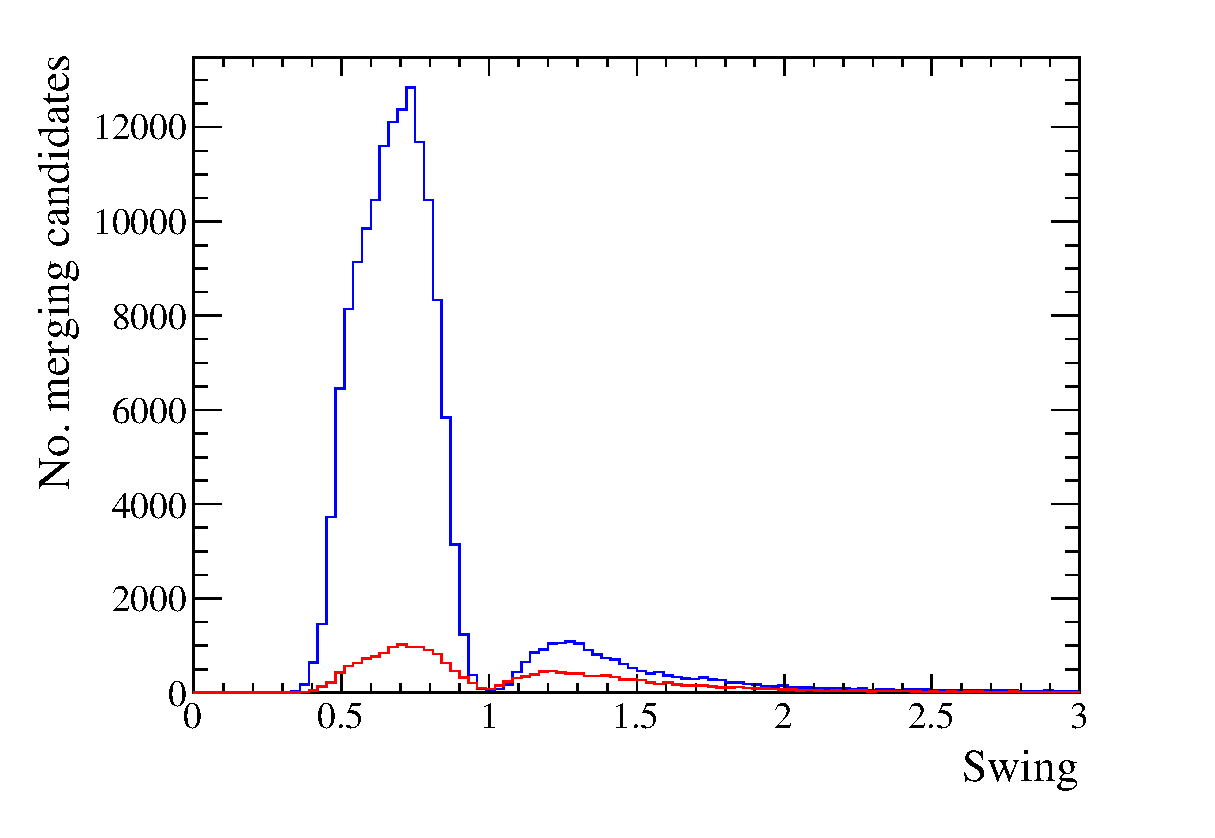
\includegraphics[width=7cm]{images/selection/vertex_recon/merging_candidates_swing_OtherCutsApplied.eps} \label{fig:TrackMergingSwingOtherCutsApplied}}
  \caption{The number of merging candidates as a function of the swing parameter.  The correct matches and incorrect matches are the blue and red histograms respectively.}
  \label{fig:TrackMergingSwing}
\end{figure}
\begin{table}[b!]
  \begin{tabular}{ c c c }
    $\cos\theta$ & Distance ratio & swing \\ \hline \hline
    $>$ 0.82 & $<$ 0.32 & $<$ 1 \\
  \end{tabular}
  \caption{Cut values for the track merging in the ECal.}
  \label{table:TrackMergingParameters}
\end{table}
\newline
\newline
All of the merging conditions have now been identified and the associated cut values are summarised in table~\ref{table:TrackMergingParameters}.

%To identify which merging candidates should actually be matched together, the truth information from the simulation was used.  Specfically, merging candidates which should be matched together are found by checking which particle produced the two tracks.  If a single particle produced both tracks, then the merging candidate is tagged as signal, otherwise it is background.


%\section{Data selection}
%Data flags

\section{Monte Carlo selection}
As briefly described at the start of this chapter, the selection separates the reconstructed ECal events into a set of topologies, where each topology is defined by a number of associated prongs.  In addition to this separation, the geometrical differences between the barrel and DS ECal suggest a further event separation.  The DS ECal lies perpendicular to the beam face.  So, particles from neutrino interactions will typically travel at right angles to the DS ECal face.  Conversely, all of the barrel ECals lie parallel to the beam axis which means neutrino interaction products will generally pass along the barrel scintillator planes.  This motivates a separate selection for the barrel and DS ECal.  This essentially means that there are eight individual selections to be made and tuned (1,2,3 and 4+ prong topologies in the barrel and 1,2,3 and 4+ prong topologies in the DS ECal).  Clearly, this approach can very quickly become complicated.  To mitigate this, similar discriminators are used for each topology.  As the reconstruction was only tuned for three reconstructed tracks, the 4+ prong topology will use exactly the same cuts as the 3 prong topology.
\newline
\newline
Care must be taken when defining what a reconstructed vertex is.  For the 2,3 and 4+ prong topologies, it is fairly simple, the reconstructed vertex is as described in section~\ref{sec:VertexReconstruction}, but it is not possible to fit for a vertex position when dealing with a single prong.  In fact, there is actually little that can be done about this.  So, beam kinematics are assumed and the 'vertex' for a single prong is the most upstream end of said prong.
\newline
\newline
The definition of signal has already been described in section~\ref{sec:SignalDefinition}.  However, how the reconstructed events map to the signal interactions also needs discussion.  The selection takes place at the reconstructed vertex level but there is not a clear 1:1 map of reconstructed vertices to signal interactions.  Consider a signal interaction in an ECal module in which the final state particles are involved in one or more secondary interactions.  The most likely outcome of this is the reconstruction of two or more vertices: one for the neutrino interaction and one or more for the secondary interactions.  By interrogating the associated truth information, each vertex will be matched to the same signal neutrino.  It is wholly incorrect to classify each vertex as a reconstruction of a signal event as this will lead to a gross overestimate of the signal rate.  To alleviate this,  a reconstructed vertex is only tagged as coming from a signal interaction if it obeys the following conditions:
\begin{itemize}
  \item The reconstructed vertex is matched to a signal interaction
  \item The reconstructed vertex is the one closest in space to the matched signal interaction
\end{itemize}
Any reconstructed vertices which pass the first condition but fail the second are tagged as a special case of background events (hereafter referred to as the 'split signal' background).
\newline
\newline
To illustrate the benefit of separating events into specific prong topologies, Fig.~\ref{fig:ProngStackAll} shows the truth makeup of events seen in the ECal after applying the reconstruction separation.  It is important to note that only the vertex reconstruction and track merging has been applied to the sample at this point.  There is a clear difference in the level of backgrounds seen in each topology e.g. the ECal OOFV background is almost exclusively contained in the one prong topology.  By applying such a separation and then focusing cuts on each topology, the overall event purity should be higher. 
\begin{figure}
  \centering
  \subfloat[Barrel ECals.]{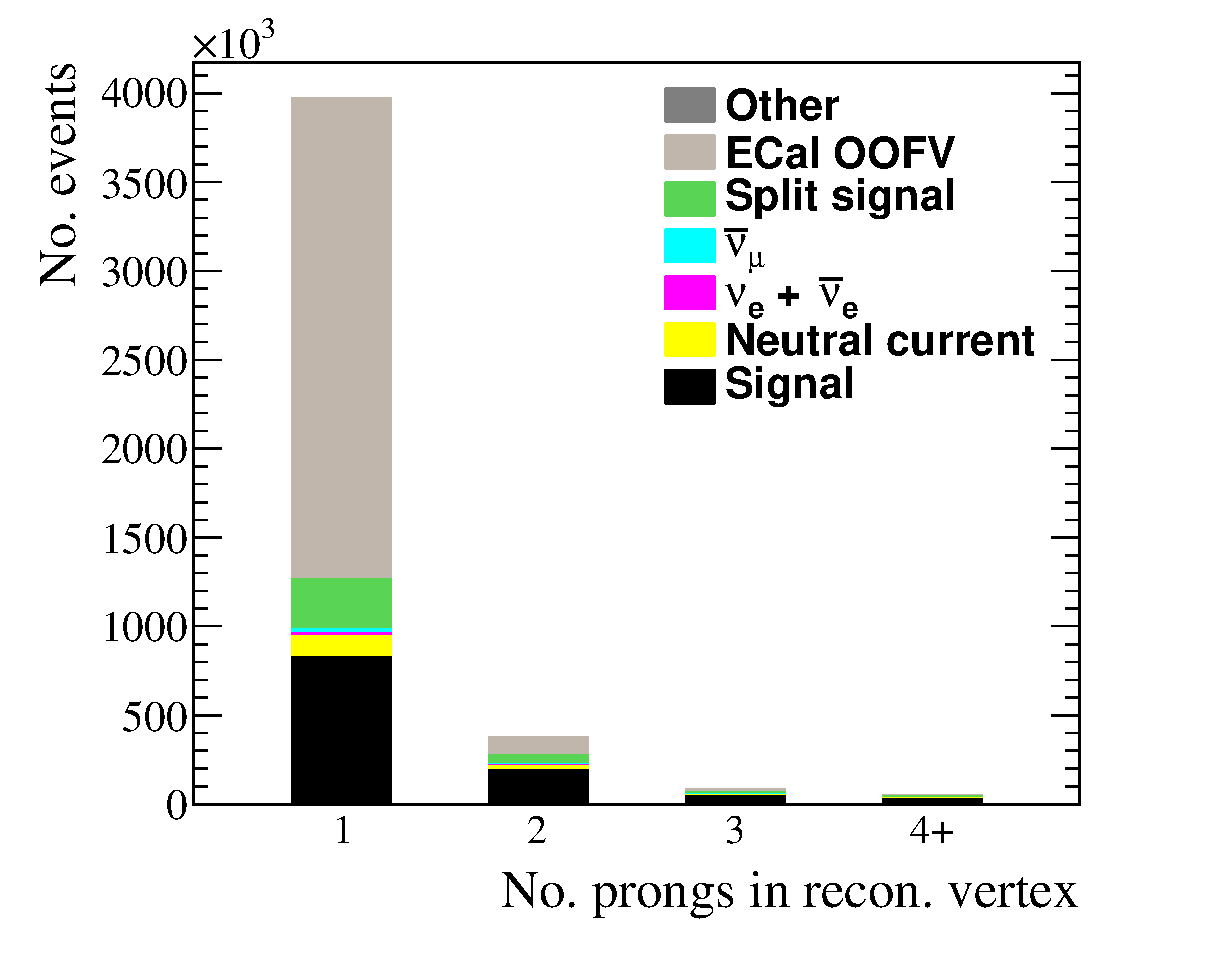
\includegraphics[width=8cm]{images/selection/mc_selection/ProngStack_Barrel_All.eps} \label{fig:ProngStackBarrelAll}}
  \subfloat[DS ECal.]{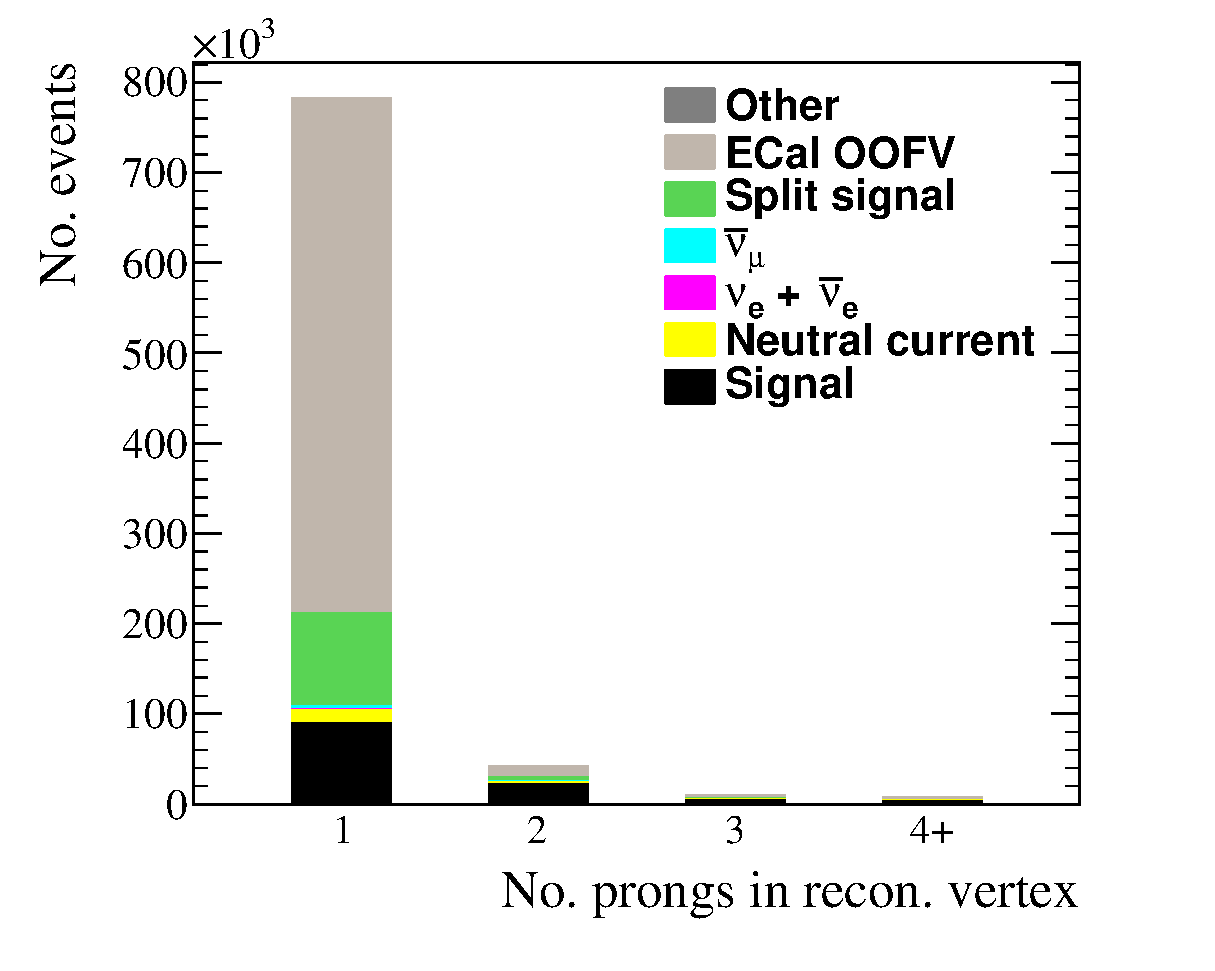
\includegraphics[width=8cm]{images/selection/mc_selection/ProngStack_DS_All.eps} \label{fig:ProngStackDSAll}}
  \caption{The number of reconstructed events in the Monte Carlo sample, separated into the prong topologies.  Each event is categorised by the associated truth information from the simulation.}
  \label{fig:ProngStackAll}
\end{figure}
\subsection{Selection cuts}
\label{subsec:SelectionCuts}
The enhanced reconstruction was developed with an ECal cross-section analysis in mind.  So, most of complex work should already have been handled by the reconstruction aspect of the analysis.  In addition, the selection method discussed involves separating events into prong topologies and focusing individual selections on each.  These points motivate a simple, cut-based, selection.  Some cuts will inevitably require some tuning and a metric is often useful for this purpose.  As demonstrated in section~\ref{sec:MonteCarloSample}, a high level of stats is seen in each ECal module which means the selection can safely strive for quality over quantity without inflating the final uncertainty.  Bearing this in mind, the metric used for tuning for prong topology $i$ is
\begin{equation}
  \phi_i^{\textrm{selection}} = \epsilon_i\eta^2_i,
  \label{eqn:SelectionMetric}
\end{equation}
where $\epsilon_i$ and $\eta_i$ are the selection efficiency and purity of prong topology $i$.  Six selection cuts have been identified which will now be discussed. 

\subsubsection{Fiducial volume cut}
\label{subsubsec:FVCut}
The first cut, the fiducial volume cut, removes most of the ECal OOFV backgrounds in the Monte Carlo sample.  This is achieved by defining some outer veto region in which occurring vertices are rejected.  There are two items to bear in mind when defining what the fiducial volumes are.  Firstly, the off-axis configuration causes each ECal to be exposed to a different energy and particle rate.  A good example of this was shown in Fig.~\ref{fig:NSignalEventsTruthNeutrinoEnergy} which shows a higher event rate, but also a higher peak energy of interactions, in the bottom-left ECal than in the top-right ECal.  So, the optimised fiducial volume of one ECal need not be the same as another ECal module.  Separately to this, Fig.~\ref{fig:ProngStackAll} shows that the ECal OOFV is almost completely contained in the 1 prong topology bin.  This means that a separate fiducial volume definition should be used for the 1 prong topology (it is sufficient for the 2,3 and 4+ prong topologies to use the same fiducial volume definition).
\newline
\newline
\begin{figure}
  \centering
  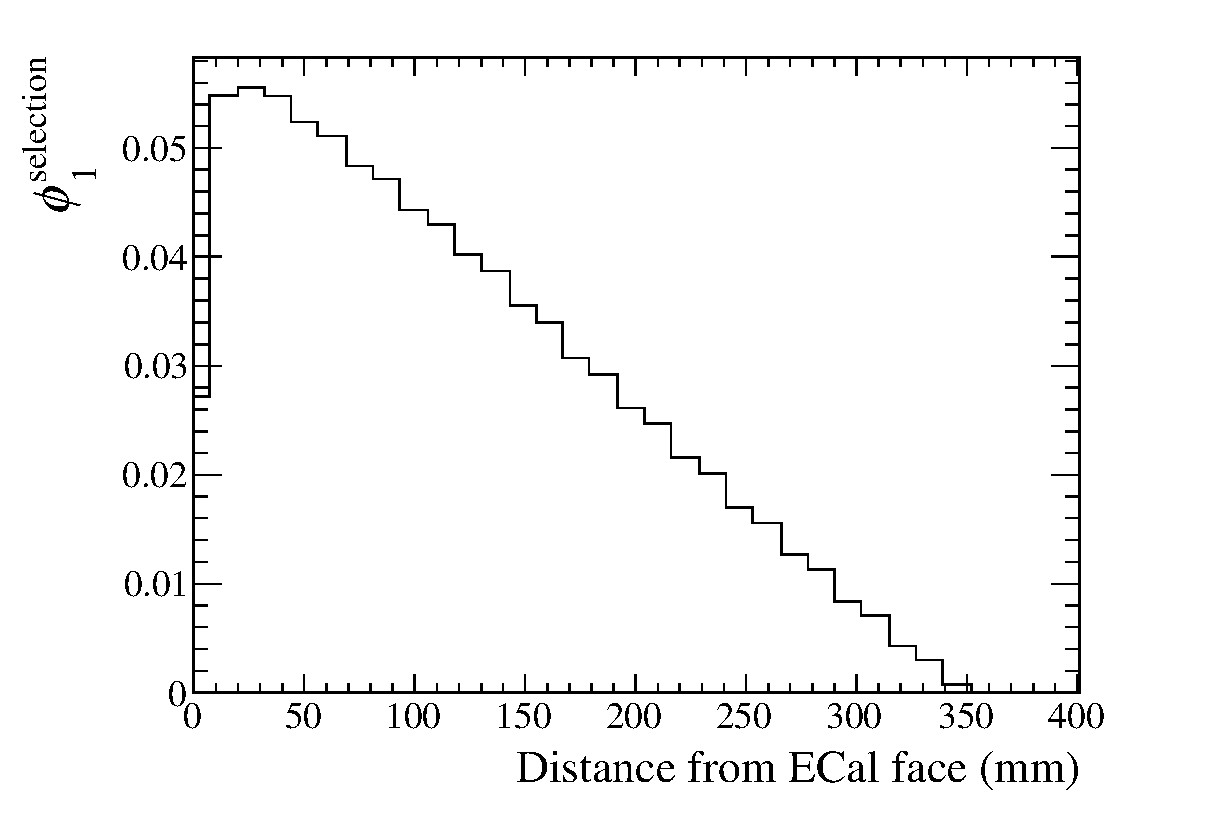
\includegraphics[width=12cm]{images/selection/mc_selection/FV_BLB_1Prong_NegY.eps}
  \caption{$\phi_i^{\textrm{selection}}$ as a function of the distance from the $-y$ face of the bottom-left barrel ECal for the 1 prong topology.}
  \label{fig:FVBLB1ProngNegY}
\end{figure}
The fiducial volume for a prong topology/ECal module is defined in terms of the distance from each face of the module.  So, there are six numbers which define the fiducial volume:  the distance from the $\pm x$,$\pm y$ and $\pm z$ faces of a module.  If the distance of a vertex from each ECal face is further than what the fiducial volume defines, the event passes the cut, otherwise it is rejected.  To tune these values,  each fiducial volume value was systematically increased from 0 mm to 600 mm in 1~mm increments.  At each increment the number of passing/rejected events was recorded and $\phi_i^{\textrm{selection}}$ calculated.  The fiducial volume value which maximises $\phi_i^{\textrm{selection}}$ is accepted as the optimised value.  An example of the variation in $\phi_i^{\textrm{selection}}$ is shown in Fig.~\ref{fig:FVBLB1ProngNegY} which shows $\phi_i^{\textrm{selection}}$ as a function of the distance from the $-y$ face of the bottom-left barrel ECal for the 1 prong topology.  There is a clear maximum found which shows the process is effective in finding an optimum distance from the ECal face.
\newline
\newline
The found fiducial volumes for each ECal module for the 1 prong topology are shown in table~\ref{table:FV1Prong}.  While all of the ECal face cuts have some discriminatory power, those which cut out according to layer number reject the most background events.  Those cuts are the $\pm y$ cuts for the bottom/top barrel ECals, the $\pm x$ cuts for the side ECals and the $\pm z$ cuts for the DS ECal.  In the barrel ECals, the inner and outer two layers are removed by the fiducial volume cut and in the DS ECal, the inner and outer three layers are removed.
\begin{table}[t!]
  \begin{tabular}{ c c c c c c c }
     & $-x$ (mm) & $+x$ (mm) & $-y$ (mm) & $+y$ (mm) & $-z$ (mm) & $+z$ (mm)  \\ \hline \hline
    Bottom-right & 36 & 36 & 31 & 29 & 206 & 28 \\
    Side-right & 31 & 29 & 46 & 44 & 206 & 28 \\
    Top-right & 39 & 27 & 29 & 31 & 172 & 28 \\
    Bottom-left & 25 & 50 & 31 & 29 & 205 & 28 \\
    Side-left & 29 & 31 & 50 & 25 & 207 & 28 \\
    Top-left & 21 & 34 & 29 & 31 & 207 & 28 \\
    Downstream & 29 & 29 & 29 & 30 & 41 & 43  \\
  \end{tabular}
  \caption{The fiducial volume definitions for each ECal module for the 1 prong topology.}
  \label{table:FV1Prong}
\end{table}
As described above, the same fiducial volumes are used for the 2,3 and 4+ prong topologies.  So, to tune the fiducial volume cuts, the topologies are temporarily combined and the combined sample is used to tune the cuts.  Those fiducial volume cuts are shown in table~\ref{table:FV2+Prong}.  There are clear differences between the fiducial volumes shown in table~\ref{table:FV1Prong} and table~\ref{table:FV2+Prong}.  The cuts suggested by the 2,3 and 4+ prong topology tunings are not as strict as those suggested by the 1 prong topology.  This should be expected, as ECal OOFV backgrounds reconstructed as 2,3 or 4+ prong vertices will most likely not have their vertex reconstructed near the faces of an ECal module.  The one exception to this is the downstream face of each ECal module.  It is clear from table~\ref{table:FV1Prong}, that the 2,3 and 4+ prong topologies suggest a stricter downstream face cut ($+z$ cut) than the 1 prong topology.  The reason for this strict cut is due to the nature of the neutrino beam.  J-PARC's neutrino beam is (almost) parallel with the $+z$ axis defined by the ND280 coordinate system.  Because of the very forward nature of the beam, any final state particles from ECal neutrino interactions are most likely to travel downstream.  So, any subsequent secondary interactions, which are tagged as background, will also occur downstream.  The $+z$ face cut attempts to remove these.
\begin{table}[b!]
  \begin{tabular}{ c c c c c c c }
     & $-x$ (mm) & $+x$ (mm) & $-y$ (mm) & $+y$ (mm) & $-z$ (mm) & $+z$ (mm)  \\ \hline \hline
    Bottom-right & 19 & 9 & 16 & 0 & 3 & 39 \\
    Side-right & 20 & 0 & 6 & 9 & 7 & 65 \\
    Top-right & 15 & 9 & 4 & 3 & 5 & 38 \\
    Bottom-left & 11 & 1 & 34 & 0 & 9 & 69 \\
    Side-left & 1 & 4 & 13 & 1 & 3 & 67 \\
    Top-left & 11 & 0 & 0 & 7 & 4 & 45 \\
    Downstream & 13 & 9 & 13 & 4 & 0 & 64  \\
  \end{tabular}
  \caption{The fiducial volume definitions for each ECal module for the 2,3 and 4+ prong topologies.}
  \label{table:FV2+Prong}
\end{table}
\subsubsection{Visible energy cut}
\label{subsubsec:VisibleEnergyCut}
The second cut rejects events based on the amount of deposited charge which is associated to the constituent prongs. The focus of this cut is to remove particle showers (typically $e^\pm$ and $\gamma$) which have been reconstructed as a vertex.  For the one prong topology, this information is trivial to evaluate: find which scintillator hits are associated to the single prong and sum their respective charge deposit.  The situation is not as clear for a vertex with multiple prongs associated.  The variable chosen in this case is the total charge associated to all of the constituent prongs.  To further increase the power of this variable as a discriminator, the total prong charge is compared to the total number of scintillator hits associated to the prongs.  The aim is to find a 2 dimensional cut which rejects events based on their associated charge and hit information.
\newline
\newline
The signal and background distributions for the barrel ECal, 1 prong topology are shown in Fig.~\ref{fig:Sel1ProngChargeVsProngNHitsSignal} and Fig.~\ref{fig:Sel1ProngChargeVsProngNHitsBackground} respectively.  To illuminate the separation power, the background/signal ratio is shown in Fig.~\ref{fig:Sel1ProngChargeVsProngNHitsRatio}, with the ratio truncated at 2.  By applying the truncation, areas where the background contamination is at least two times as large as the signal population is easily found.  To develop the 2 dimensional cuts, a test line is drawn which appears to roughly cut out the highly contaminated (red) areas in Fig.~\ref{fig:Sel1ProngChargeVsProngNHitsRatio}.  Then, to tune the cut line, the parameters of said line are varied in a grid search.  At each point in the grid, $\phi_i^{\textrm{selection}}$ is recorded.  The maximum value in this grid corresponds to the optimised parameters of the cut line.  As is evident from Fig.~\ref{fig:Sel1ProngChargeVsProngNHitsRatio}, there are two areas of high background contamination which motivated the development two cut lines which are both overlaid on Fig.~\ref{fig:Sel1ProngChargeVsProngNHitsRatio}.
\begin{figure}
\begin{minipage}{.5\linewidth}
  \centering
  \subfloat[Signal events only.]{\label{fig:Sel1ProngChargeVsProngNHitsSignal}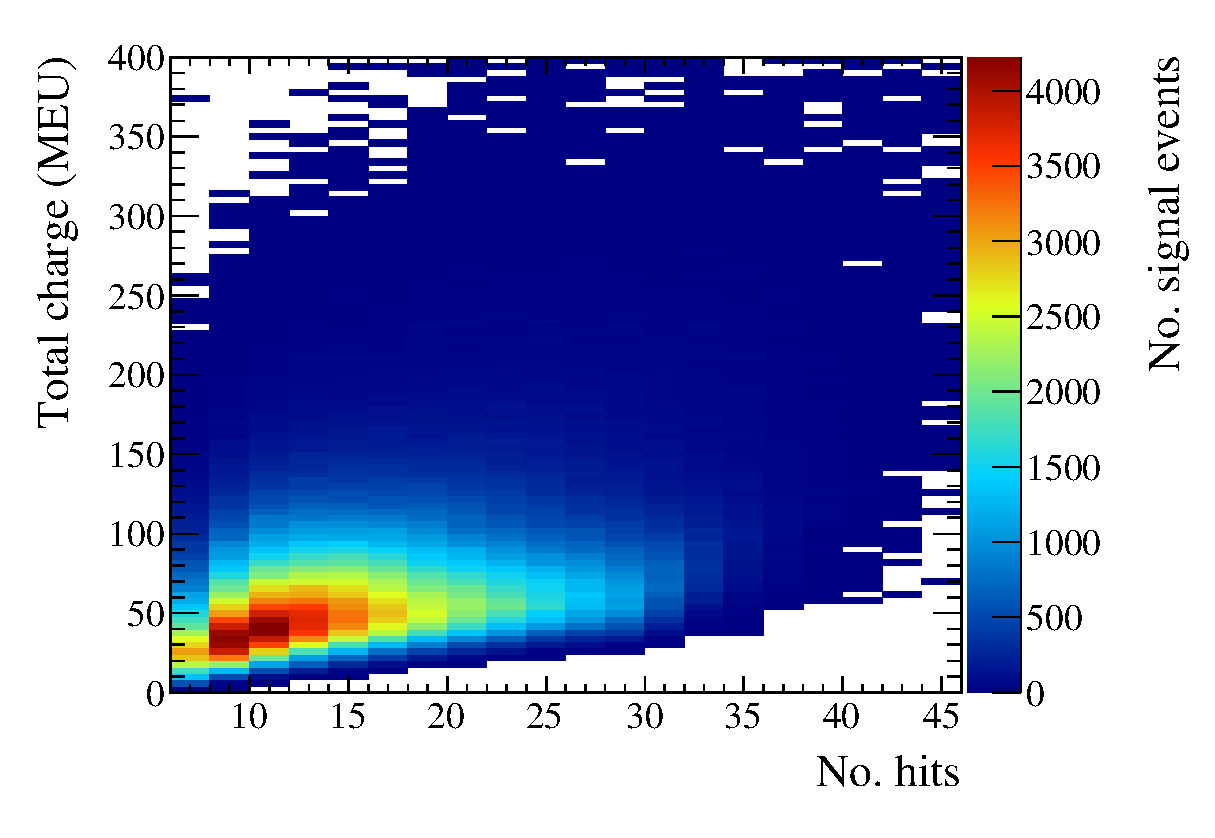
\includegraphics[width=7.5cm]{images/selection/mc_selection/ProngChargeVsNHits_1prong_barrel_signal.eps}}
\end{minipage}%
\begin{minipage}{.5\linewidth}
\centering
\subfloat[Background events only.]{\label{fig:Sel1ProngChargeVsProngNHitsBackground}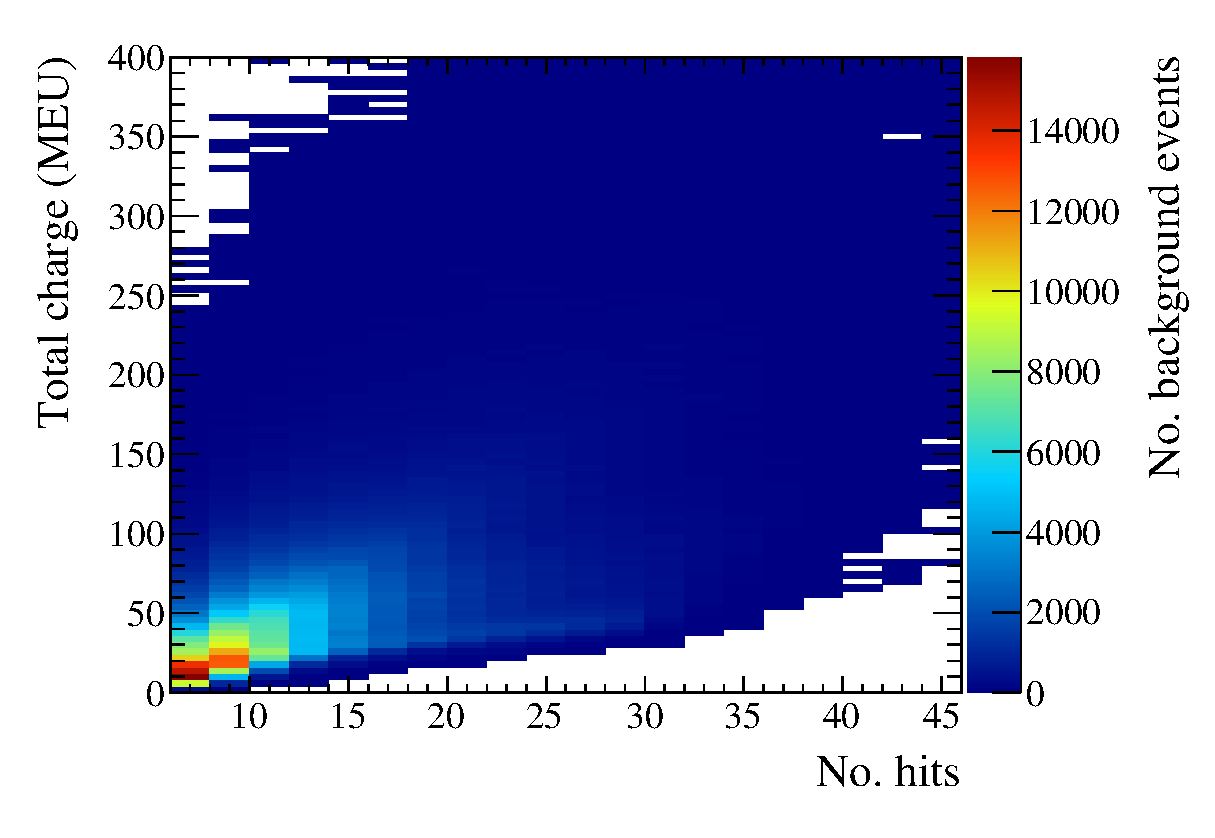
\includegraphics[width=7.5cm]{images/selection/mc_selection/ProngChargeVsNHits_1prong_barrel_background.eps}}
\end{minipage}\par\medskip
\centering
\subfloat[Background/Signal ratio, truncated at 2.  The black lines portray the cut lines and the attached arrows show which side of the cut is selected.]{\label{fig:Sel1ProngChargeVsProngNHitsRatio}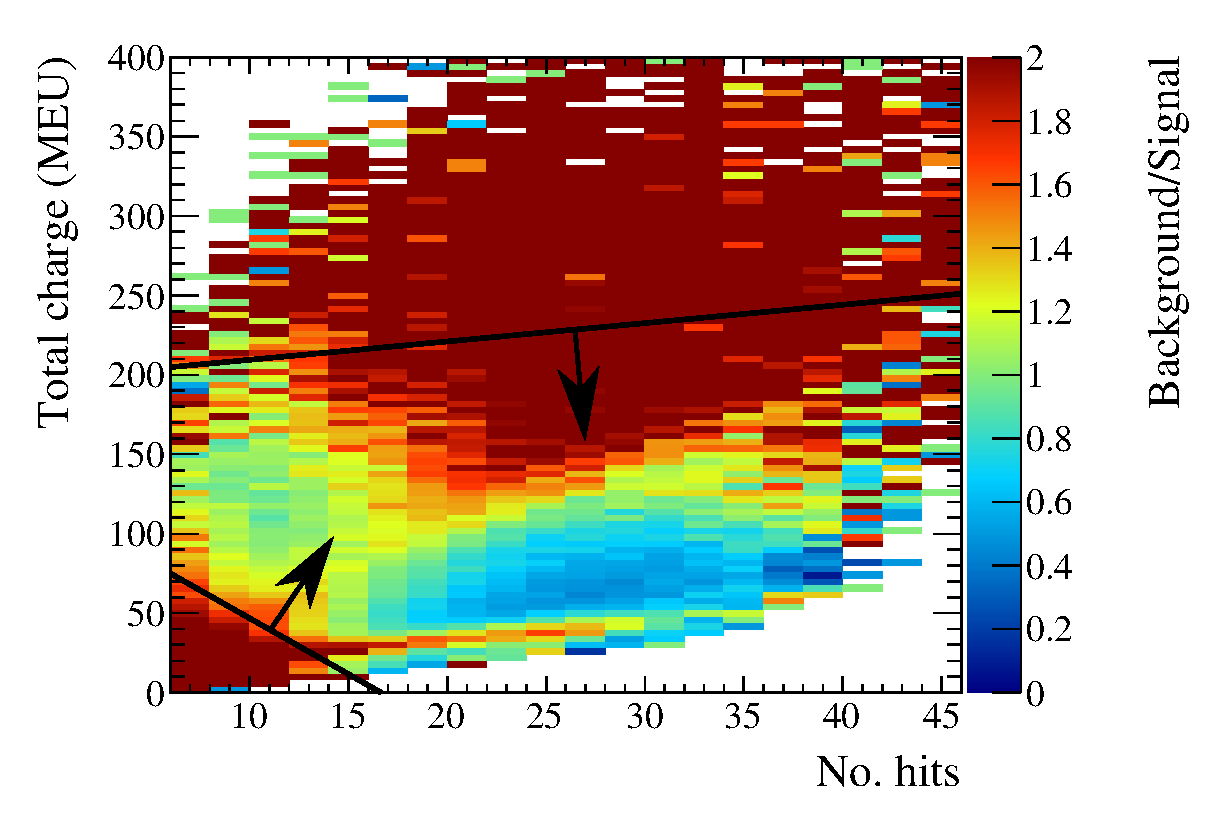
\includegraphics[width=7.5cm]{images/selection/mc_selection/ProngChargeVsNHits_1prong_barrel_ratio.eps}}
\caption{Total prong charge vs the number of prong hits for barrel ECal events in the 1 prong topology.}
\label{fig:Sel1ProngChargeVsProngNHits}
\end{figure}
\newline
\newline
Fig.~\ref{fig:Sel2ProngChargeVsProngNHits} and Fig.~\ref{fig:Sel3ProngChargeVsProngNHits} show similar distributions for the 2 and 3 prong topology in the barrel ECal.  The ratio distributions also have the cut lines overlaid.  An identical process was used to generate and tune the cut lines.  By using a definition for the total number of scintillator hits associated to all constituent prongs in a vertex, $N$, the definition of the cut lines are shown in table~\ref{table:ProngChargeVsProngNHitsCuts}.
\begin{figure}
\begin{minipage}{.5\linewidth}
  \centering
  \subfloat[Signal events only.]{\label{fig:Sel2ProngChargeVsProngNHitsSignal}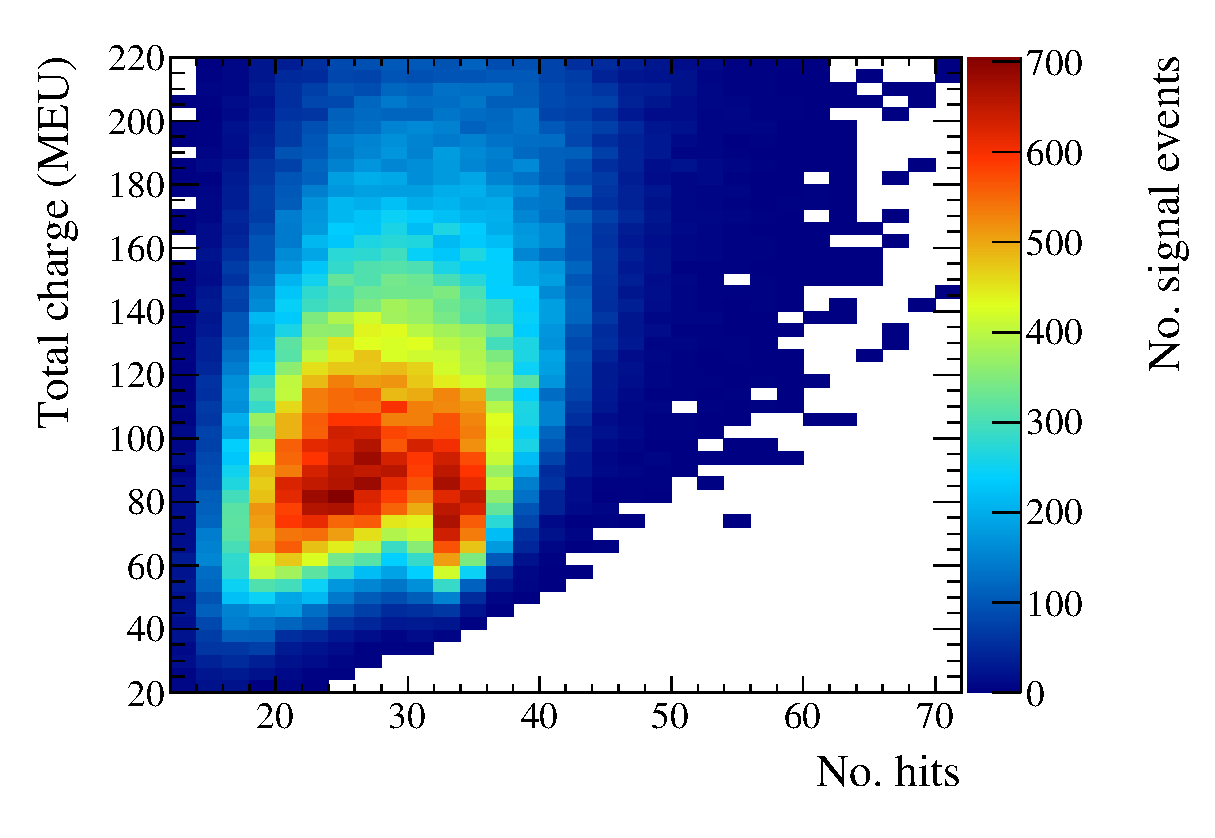
\includegraphics[width=7.5cm]{images/selection/mc_selection/ProngChargeVsNHits_2prong_barrel_signal.eps}}
\end{minipage}%
\begin{minipage}{.5\linewidth}
\centering
\subfloat[Background events only.]{\label{fig:Sel2ProngChargeVsProngNHitsBackground}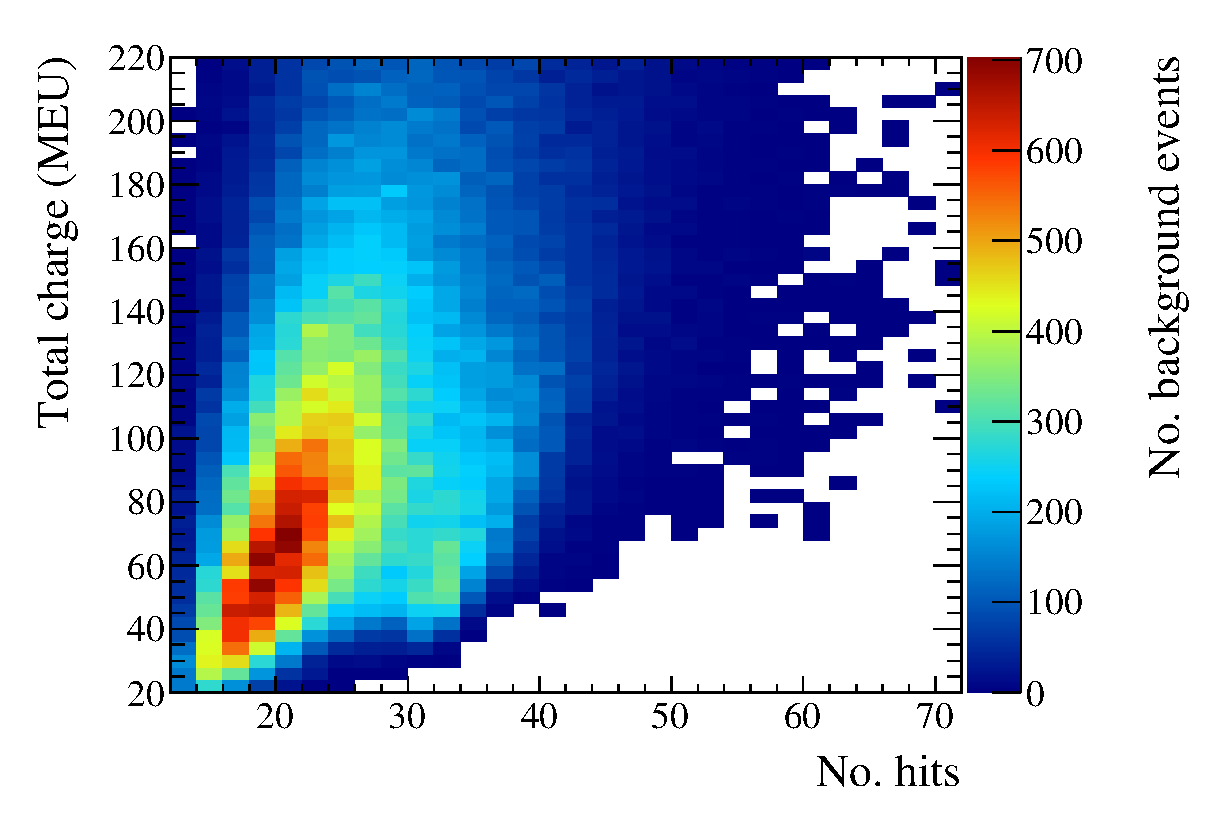
\includegraphics[width=7.5cm]{images/selection/mc_selection/ProngChargeVsNHits_2prong_barrel_background.eps}}
\end{minipage}\par\medskip
\centering
\subfloat[Background/Signal ratio, truncated at 2.  The black line portrays the cut line and the attached arrow shows which side of the cut is selected.]{\label{fig:Sel2ProngChargeVsProngNHitsRatio}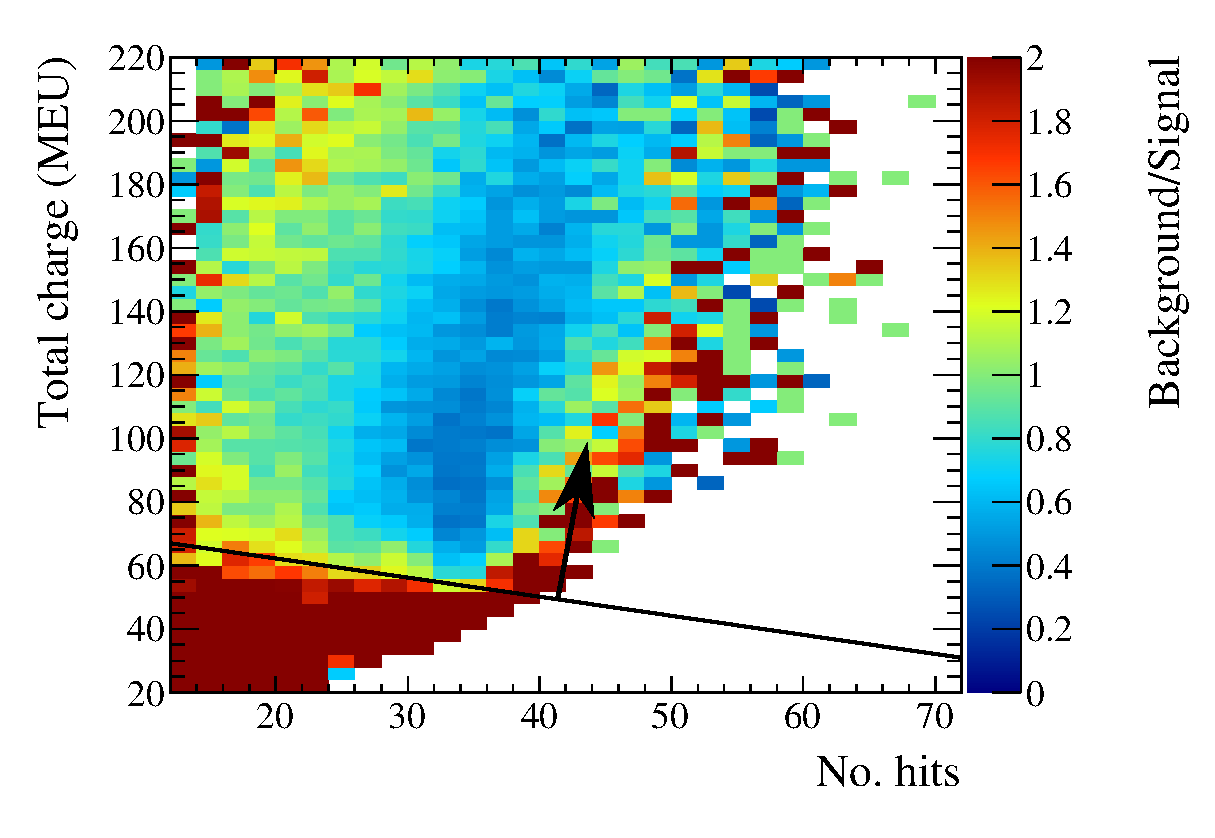
\includegraphics[width=7.5cm]{images/selection/mc_selection/ProngChargeVsNHits_2prong_barrel_ratio.eps}}
\caption{Total prong charge vs the number of prong hits for barrel ECal events in the 2 prong topology.}
\label{fig:Sel2ProngChargeVsProngNHits}
\end{figure}

\begin{figure}
\begin{minipage}{.5\linewidth}
  \centering
  \subfloat[Signal events only.]{\label{fig:Sel3ProngChargeVsProngNHitsSignal}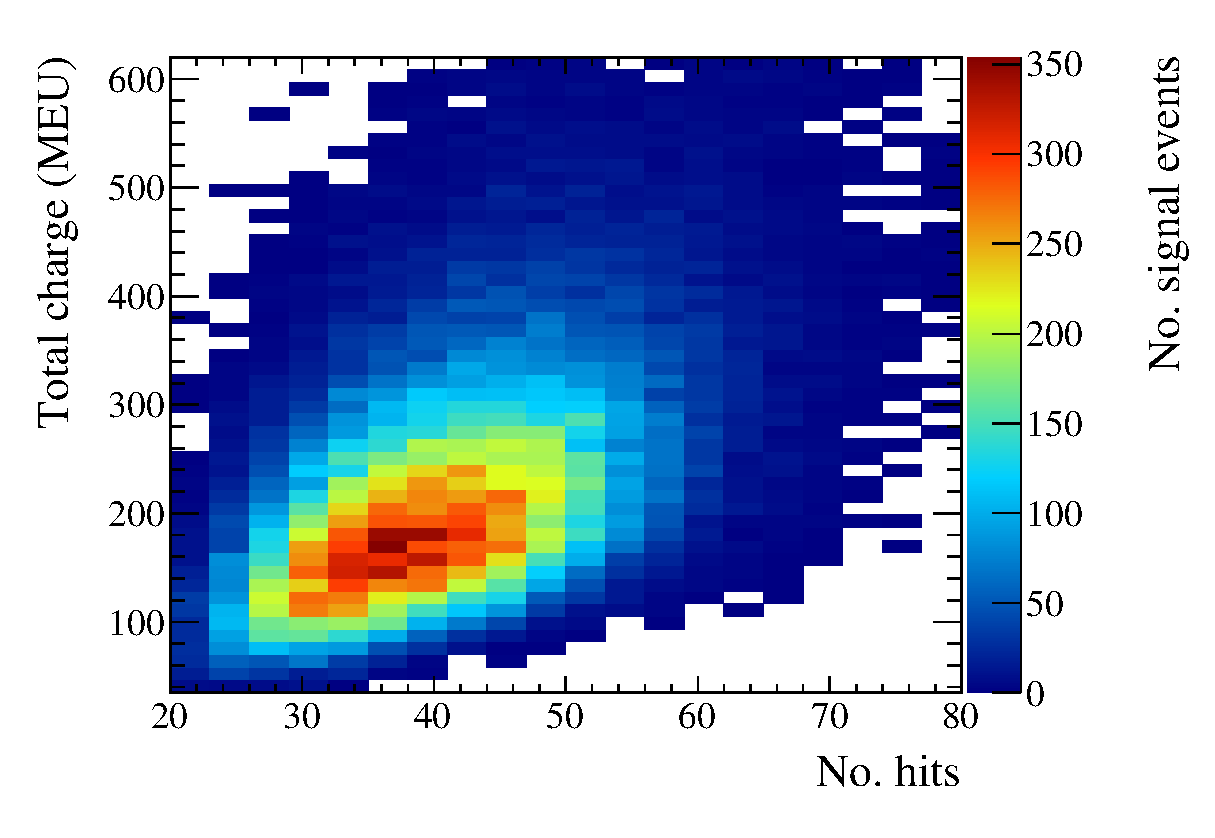
\includegraphics[width=7.5cm]{images/selection/mc_selection/ProngChargeVsNHits_3prong_barrel_signal.eps}}
\end{minipage}%
\begin{minipage}{.5\linewidth}
\centering
\subfloat[Background events only.]{\label{fig:Sel3ProngChargeVsProngNHitsBackground}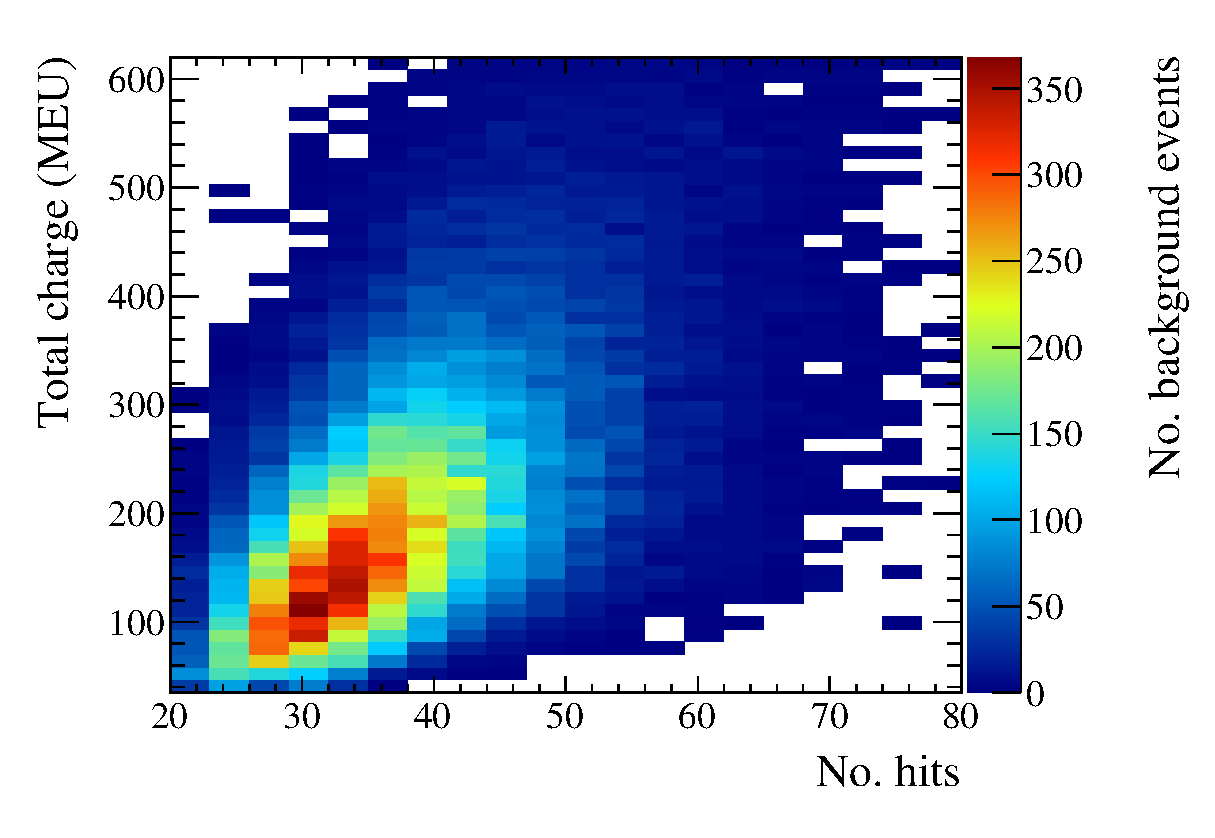
\includegraphics[width=7.5cm]{images/selection/mc_selection/ProngChargeVsNHits_3prong_barrel_background.eps}}
\end{minipage}\par\medskip
\centering
\subfloat[Background/Signal ratio, truncated at 2.  The black line portrays the cut line and the attached arrow shows which side of the cut is selected.]{\label{fig:Sel3ProngChargeVsProngNHitsRatio}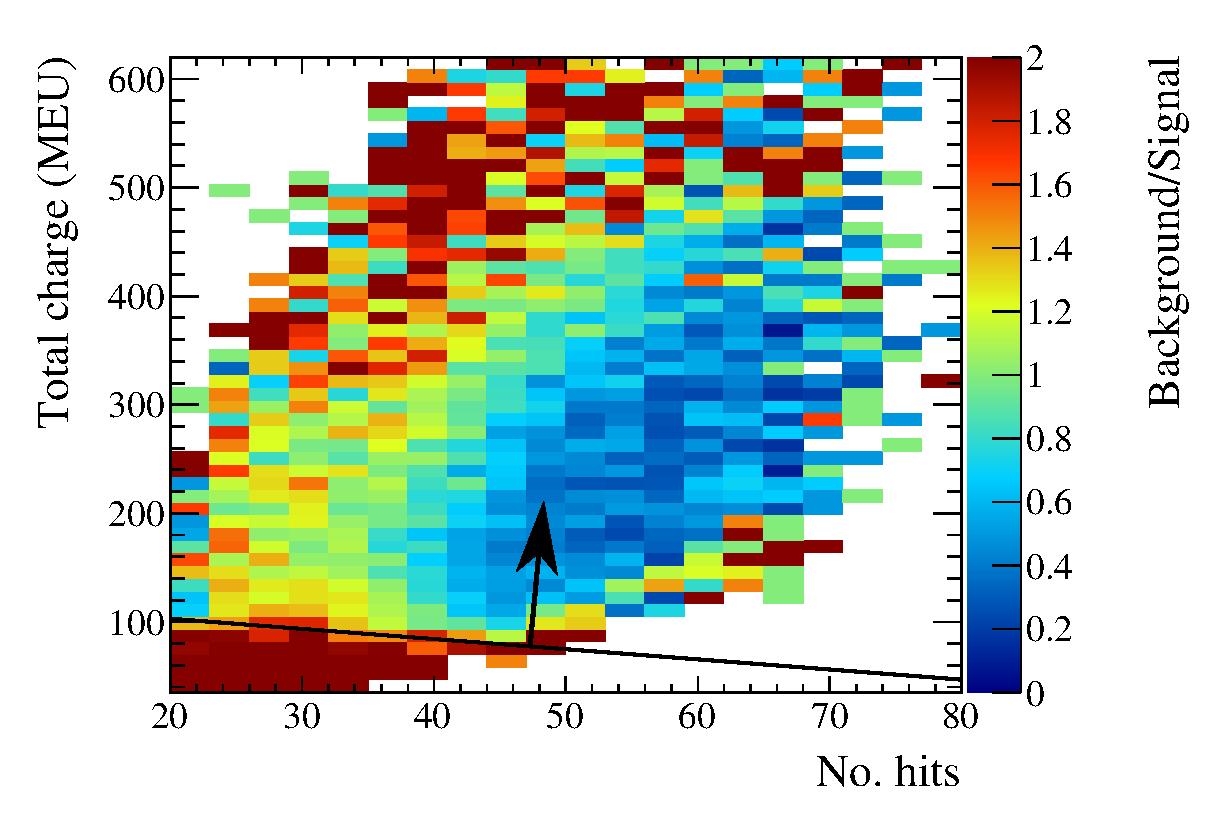
\includegraphics[width=7.5cm]{images/selection/mc_selection/ProngChargeVsNHits_3prong_barrel_ratio.eps}}
\caption{Total prong charge vs the number of prong hits for barrel ECal events in the 3 prong topology.}
\label{fig:Sel3ProngChargeVsProngNHits}
\end{figure}
\begin{table}
  \begin{tabular}{ c l l }
    Prong topology & Barrel cuts (MEU) & DS cuts (MEU) \\ \hline \hline
    1 & $>-4.5N + 75$ & $>-3.4N + 62$ \\
     &  $<N + 205$ &  \\
    2 & $>-0.5N + 67$ & $>0.2N + 51$ \\
    3 & $>0.7N + 103$ & $>-1.1N + 117$ \\
  \end{tabular}
  \caption{The definitions of the 2 dimensional cut lines involving the total prong charge and the number of associated scintillator hits. $N$ refers to the total number of scintillator hits associated to the constituent prongs in the vertex.}
  \label{table:ProngChargeVsProngNHitsCuts}
\end{table}
\subsubsection{Unused hits cut}
\label{subsubsec:UnusedHitsCuts}
The output of the enhanced reconstruction is a set of reconstructed clusters.  Within those clusters are a set of tracks and their pairwise crossings which are used to reconstruct the ECal vertices used by this analysis.  The clusters which contain the tracks and crossings can also be utilised as a discriminator.  Particle showers should generally produce a lot of hits and those hits are not necessarily arranged in a linear fashion.  So, the third cut implemented assesses how many hits are associated with a cluster but not associated with the vertex.  The vertex is defined by its prong constituents so this is really a measure of how many scintillator hits were not associated with the reconstructed prongs.  By defining the number of hits in the cluster as $N^{\textrm{Cluster}}$ and the number of hits associated with the $i^{\textrm{th}}$ constituent prong as $N^{\textrm{prong}}_i$, the discriminator is
\begin{equation}
  \Delta N = N^{\textrm{cluster}} - \sum_i N^{\textrm{prong}}_i.
  \label{eqn:DeltaNHits}
\end{equation}
The cut value really should depend on how many hits are associated to the constituent prongs.  So, as was done in section~\ref{subsubsec:VisibleEnergyCut}, the $\Delta N$ cut should be 2 dimensional.  Specifically, the $\Delta N$ cut should depend on the number of scintillator hits associated to the constituent prongs.
\newline
\newline
So, an identical approach is used to define and tune the cut lines as was used in section~\ref{subsubsec:VisibleEnergyCut}.  The signal, background and background/signal ratio distributions for the 1, 2 and 3 prong topologies in the barrel ECal are shown in Fig.~\ref{fig:Sel1DeltaNHitsVsProngNHits}, Fig.~\ref{fig:Sel2DeltaNHitsVsProngNHits} and Fig.~\ref{fig:Sel3DeltaNHitsVsProngNHits} respectively.  The layout of the figures is the same as was shown for the visible energy cut.  In a similar manner to table~\ref{table:ProngChargeVsProngNHitsCuts}, the $\Delta N$ cut definitions are shown in table~\ref{table:DeltaNHitsVsProngNHitsCuts}.
\begin{table}[!b]
  \begin{tabular}{ c l l }
    Prong topology & Barrel cuts (no units) & DS cuts (no units) \\ \hline \hline
    1 & $<-0.2N + 16$ & $<1.2N + 3$ \\
    2 & $<1.5N - 16$ & $<0.7N - 4$ \\
    3 & $<1.7N + 7$ & $<0.8N + 1$ \\
  \end{tabular}
  \caption{The definitions of the 2 dimensional cut lines involving $\Delta N$ and the number of scintillator hits associated with the constituent prongs. $N$ refers to the total number of scintillator hits associated to the constituent prongs in the vertex.}
  \label{table:DeltaNHitsVsProngNHitsCuts}
\end{table}

\begin{figure}
\begin{minipage}{.5\linewidth}
  \centering
  \subfloat[Signal events only.]{\label{fig:Sel1DeltaNHitsVsProngNHitsSignal}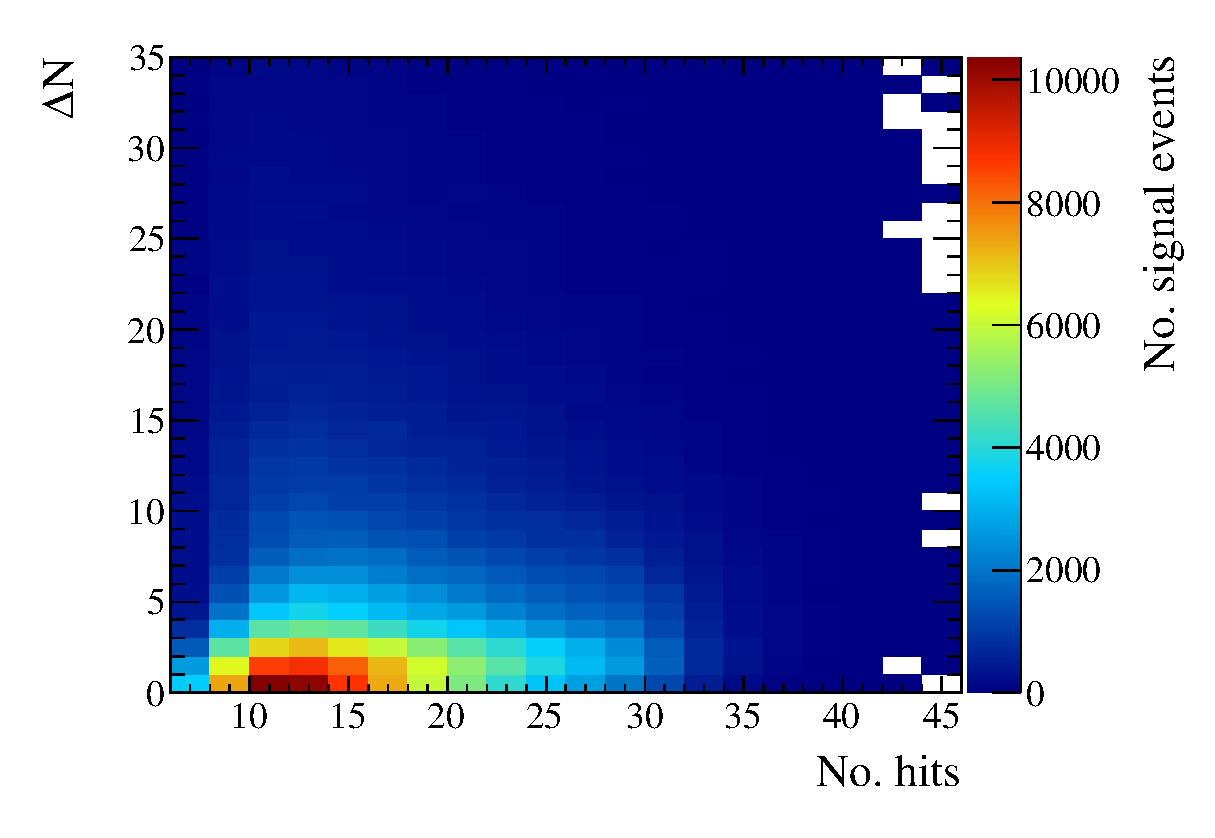
\includegraphics[width=7.5cm]{images/selection/mc_selection/DeltaNHitsVsNHits_1Prong_Barrel_signal.eps}}
\end{minipage}%
\begin{minipage}{.5\linewidth}
\centering
\subfloat[Background events only.]{\label{fig:Sel1DeltaNHitsVsProngNHitsBackground}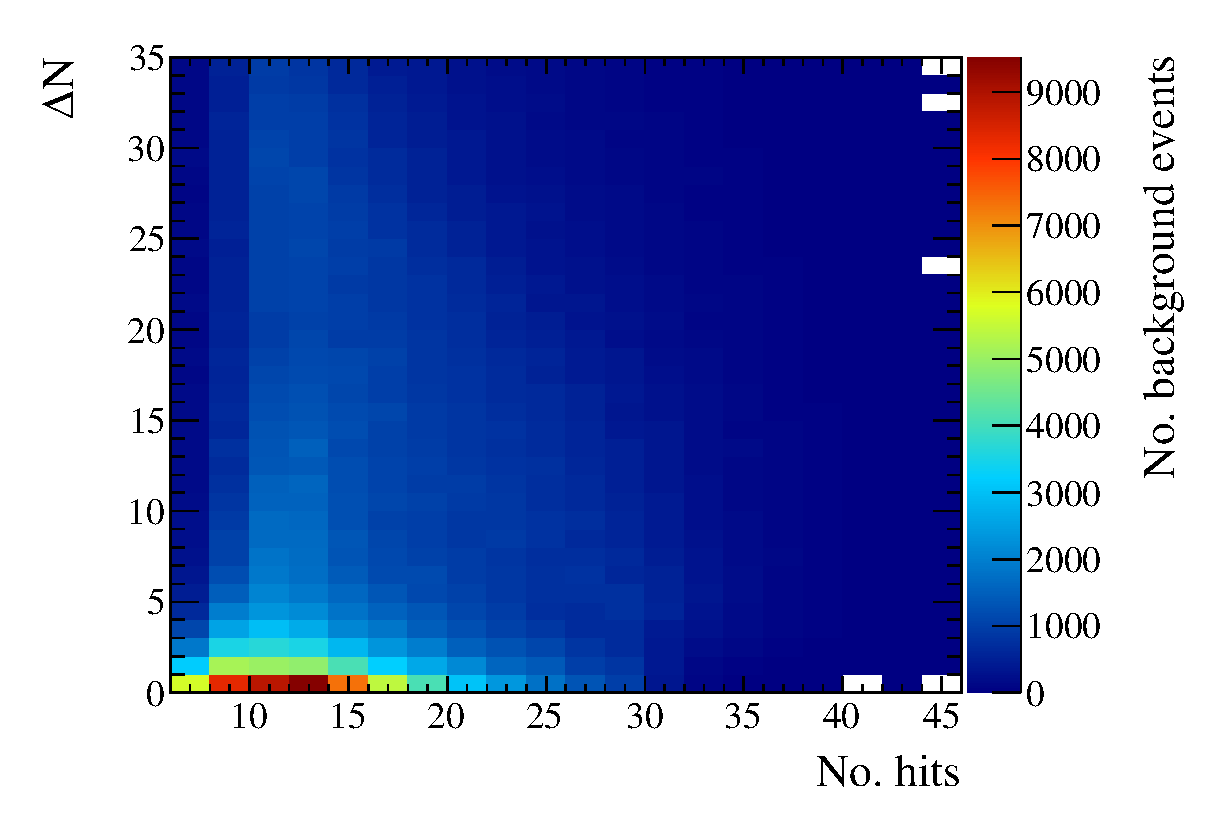
\includegraphics[width=7.5cm]{images/selection/mc_selection/DeltaNHitsVsNHits_1Prong_Barrel_background.eps}}
\end{minipage}\par\medskip
\centering
\subfloat[Background/Signal ratio, truncated at 2.  The black line portrays the cut line and the attached arrow shows which side of the cut is selected.]{\label{fig:Sel1DeltaNHitsVsProngNHitsRatio}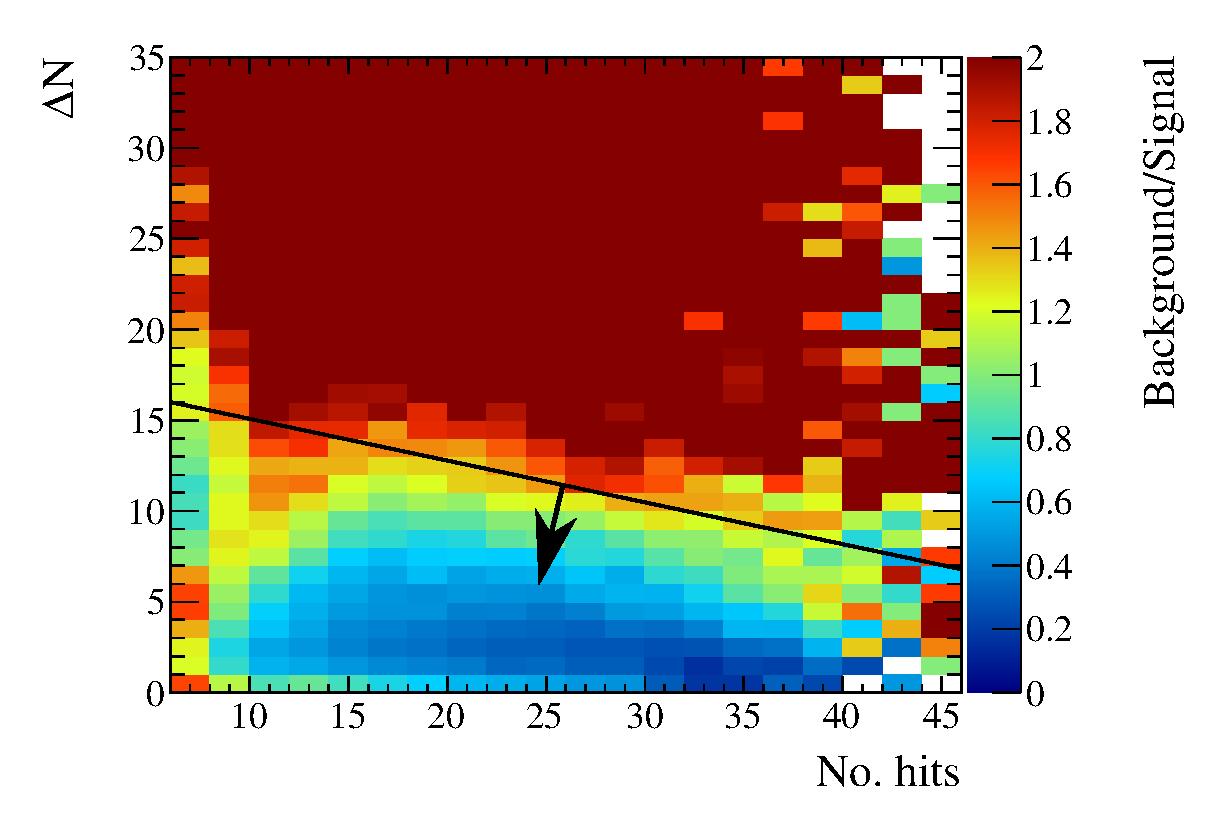
\includegraphics[width=7.5cm]{images/selection/mc_selection/DeltaNHitsVsNHits_1Prong_Barrel_ratio.eps}}
\caption{$\Delta N$ vs the number of prong hits for barrel ECal events in the 1 prong topology.}
\label{fig:Sel1DeltaNHitsVsProngNHits}
\end{figure}

\begin{figure}
\begin{minipage}{.5\linewidth}
  \centering
  \subfloat[Signal events only.]{\label{fig:Sel2DeltaNHitsVsProngNHitsSignal}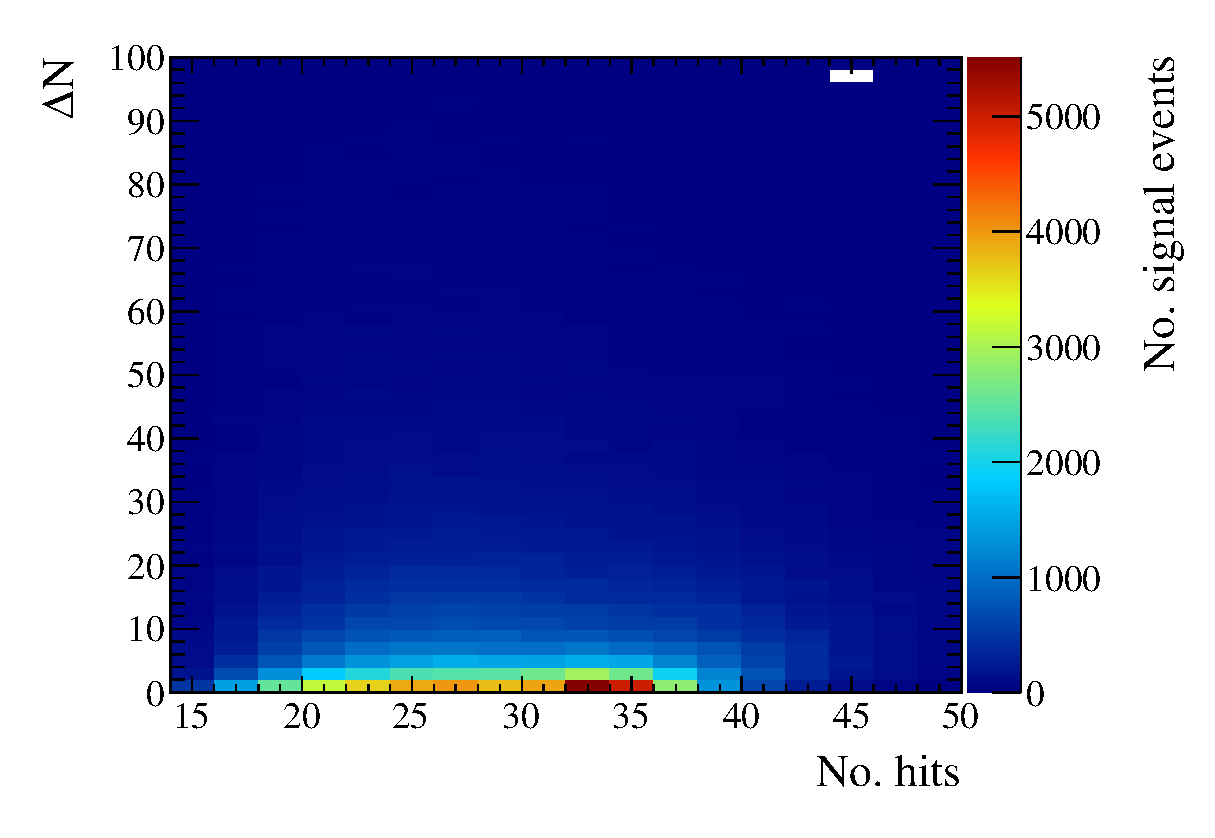
\includegraphics[width=7.5cm]{images/selection/mc_selection/DeltaNHitsVsNHits_2Prong_Barrel_signal.eps}}
\end{minipage}%
\begin{minipage}{.5\linewidth}
\centering
\subfloat[Background events only.]{\label{fig:Sel2DeltaNHitsVsProngNHitsBackground}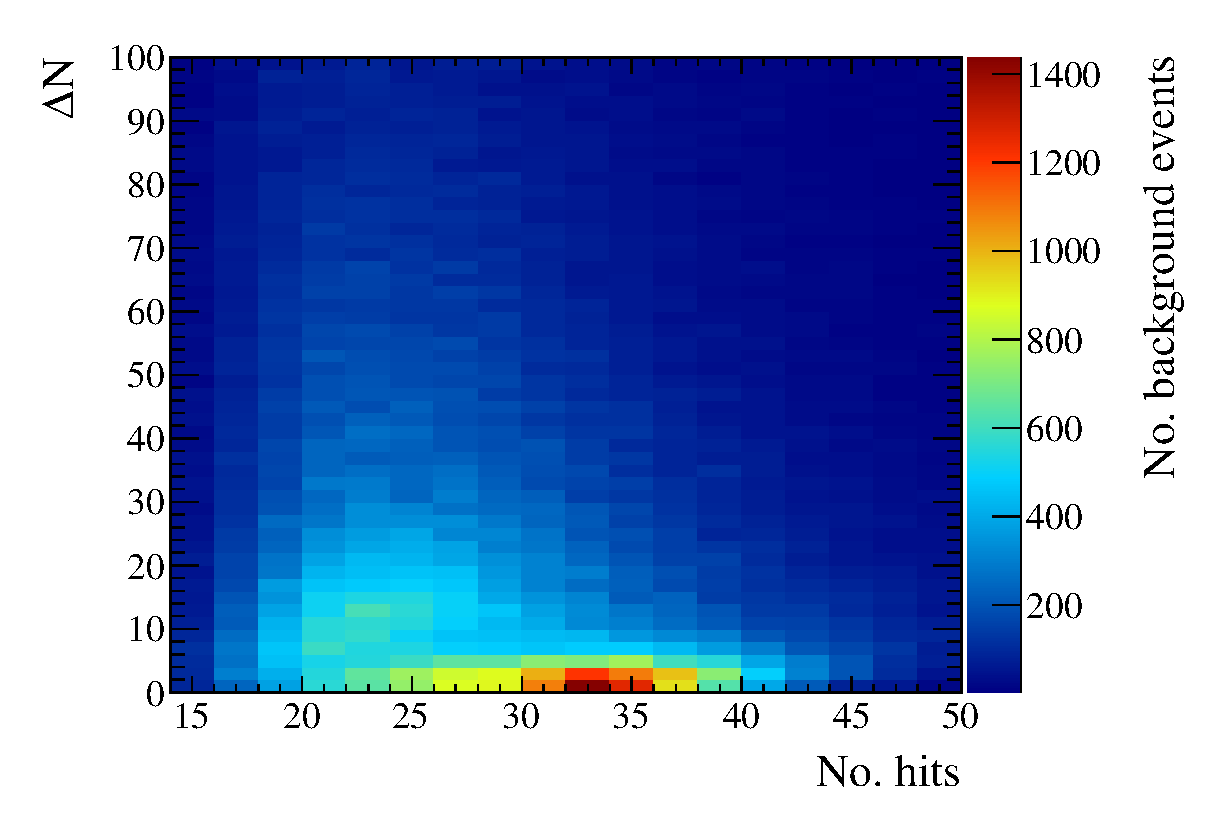
\includegraphics[width=7.5cm]{images/selection/mc_selection/DeltaNHitsVsNHits_2Prong_Barrel_background.eps}}
\end{minipage}\par\medskip
\centering
\subfloat[Background/Signal ratio, truncated at 2.  The black line portrays the cut line and the attached arrow shows which side of the cut is selected.]{\label{fig:Sel2DeltaNHitsVsProngNHitsRatio}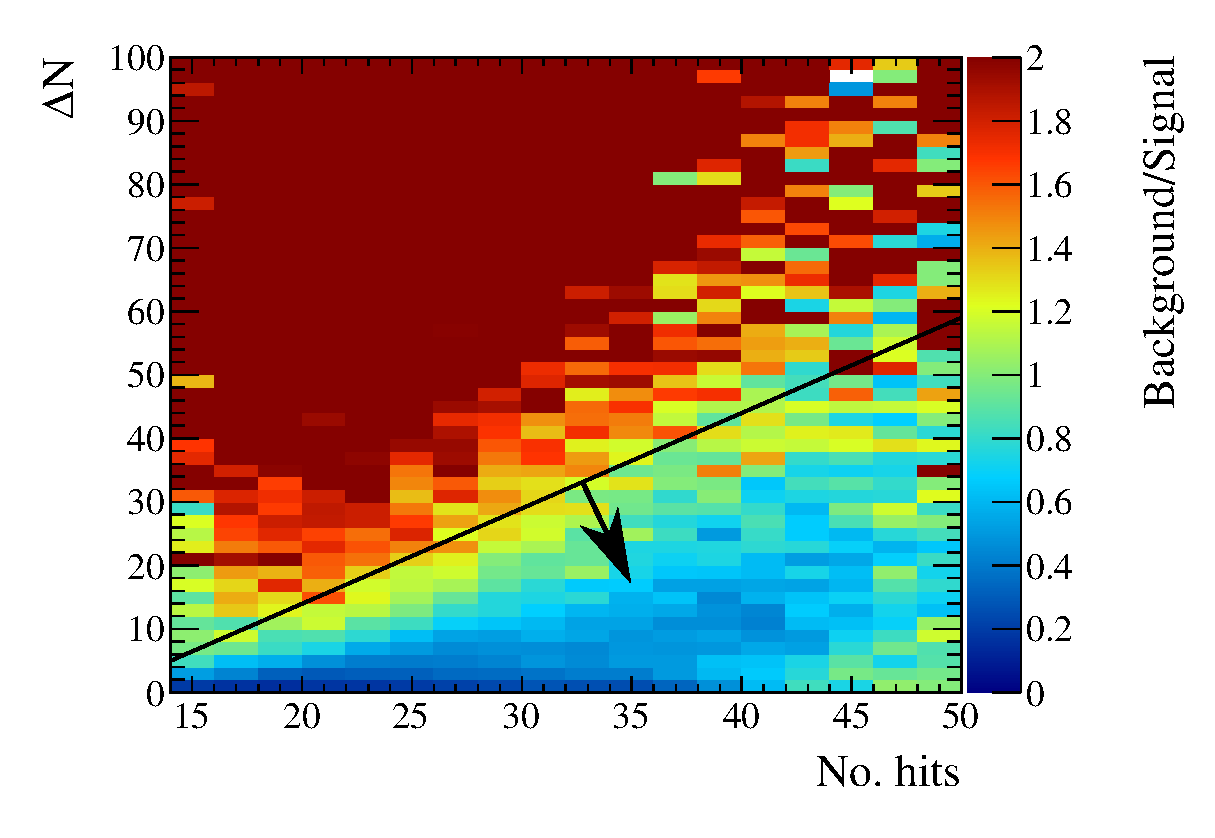
\includegraphics[width=7.5cm]{images/selection/mc_selection/DeltaNHitsVsNHits_2Prong_Barrel_ratio.eps}}
\caption{$\Delta N$ vs the number of prong hits for barrel ECal events in the 2 prong topology.}
\label{fig:Sel2DeltaNHitsVsProngNHits}
\end{figure}

\begin{figure}
\begin{minipage}{.5\linewidth}
  \centering
  \subfloat[Signal events only.]{\label{fig:Sel3DeltaNHitsVsProngNHitsSignal}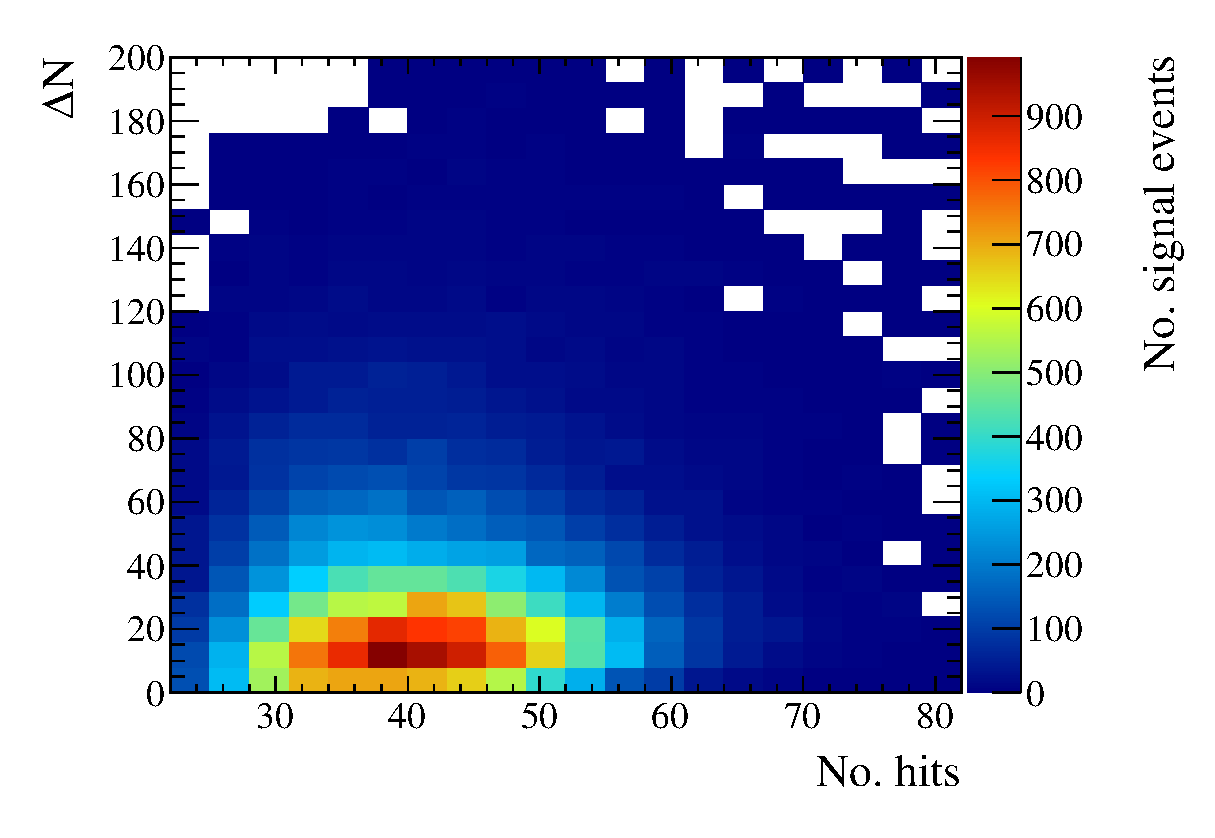
\includegraphics[width=7.5cm]{images/selection/mc_selection/DeltaNHitsVsNHits_3Prong_Barrel_signal.eps}}
\end{minipage}%
\begin{minipage}{.5\linewidth}
\centering
\subfloat[Background events only.]{\label{fig:Sel3DeltaNHitsVsProngNHitsBackground}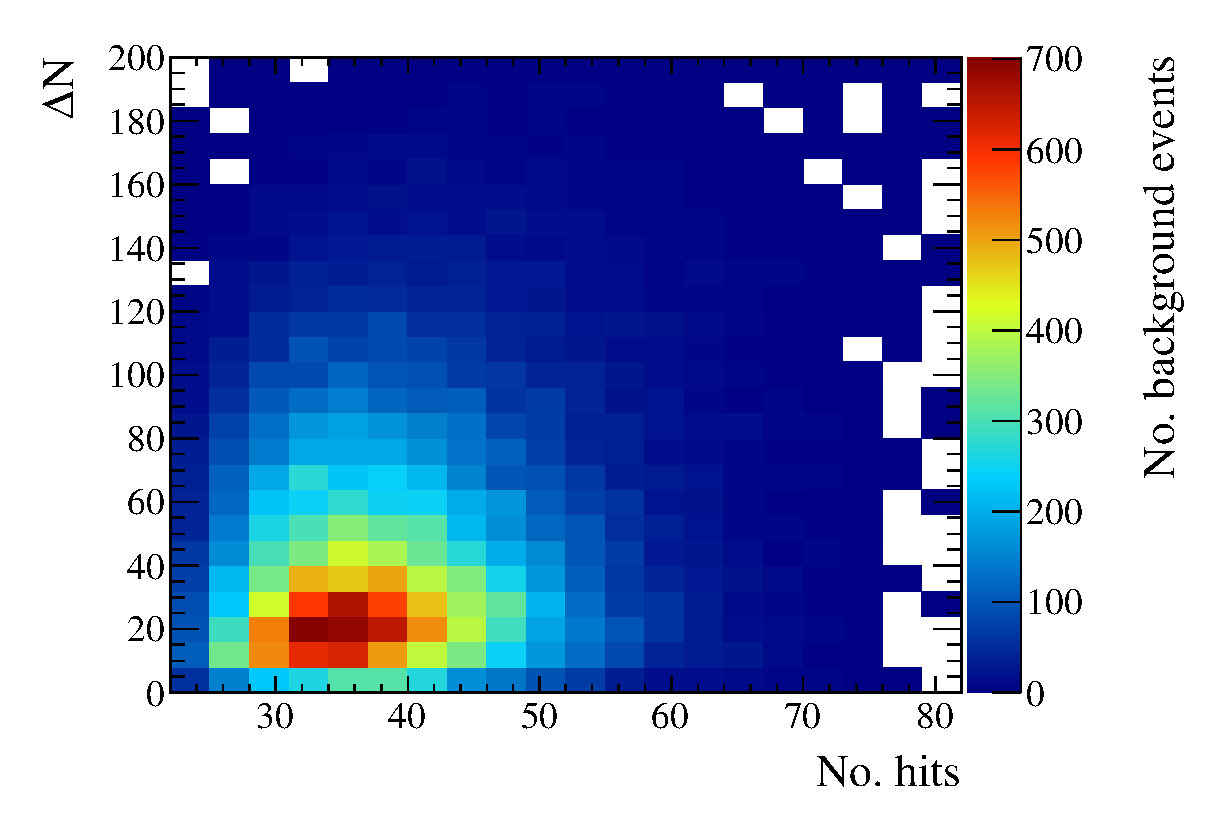
\includegraphics[width=7.5cm]{images/selection/mc_selection/DeltaNHitsVsNHits_3Prong_Barrel_background.eps}}
\end{minipage}\par\medskip
\centering
\subfloat[Background/Signal ratio, truncated at 2.  The black line portrays the cut line and the attached arrow shows which side of the cut is selected.]{\label{fig:Sel3DeltaNHitsVsProngNHitsRatio}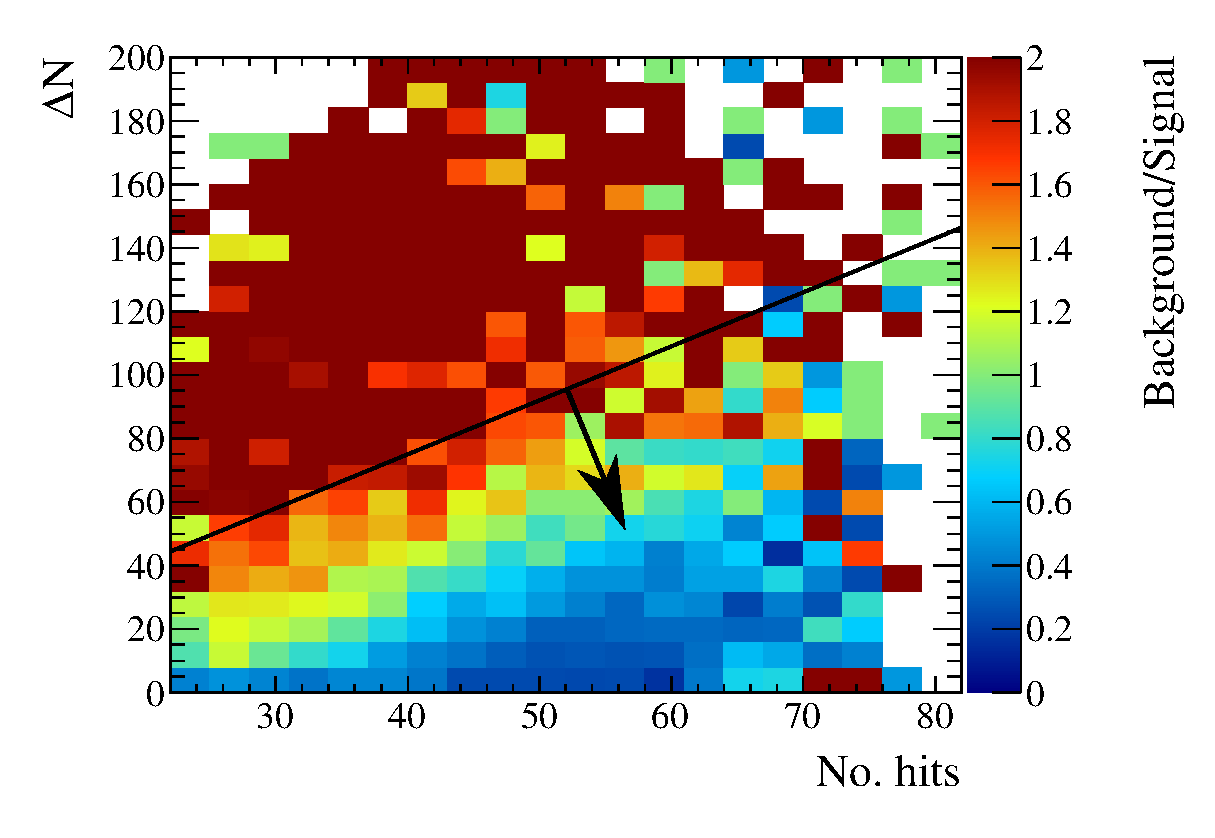
\includegraphics[width=7.5cm]{images/selection/mc_selection/DeltaNHitsVsNHits_3Prong_Barrel_ratio.eps}}
\caption{$\Delta N$ vs the number of prong hits for barrel ECal events in the 3 prong topology.}
\label{fig:Sel3DeltaNHitsVsProngNHits}
\end{figure}

\subsubsection{Opening angle}
\label{subsubsec:OpeningAngle}
Despite the best efforts of the track merging, not all curving trajectories have reconstructed tracks which are successfully merged.  So, there will be an inherent ECal OOFV contamination of the 2,3 and 4+ prong topologies where the reconstruction has failed.  While future iterations of the analysis should revisit the reconstruction to combat this, it is sufficient to cut these background events out in the selection.  As was described in section~\ref{sec:VertexReconstruction}, a key signature of a curving trajectory is two prongs with a small opening angle.  This means that the opening angle can be used as a cut to remove such background events.  To define an opening angle, at least two tracks are required so, unfortunately, such a method can not be implemented for the 1 prong topology.
\newline
\newline
\begin{figure}[b!]
  \centering
  \subfloat[Barrel ECals.]{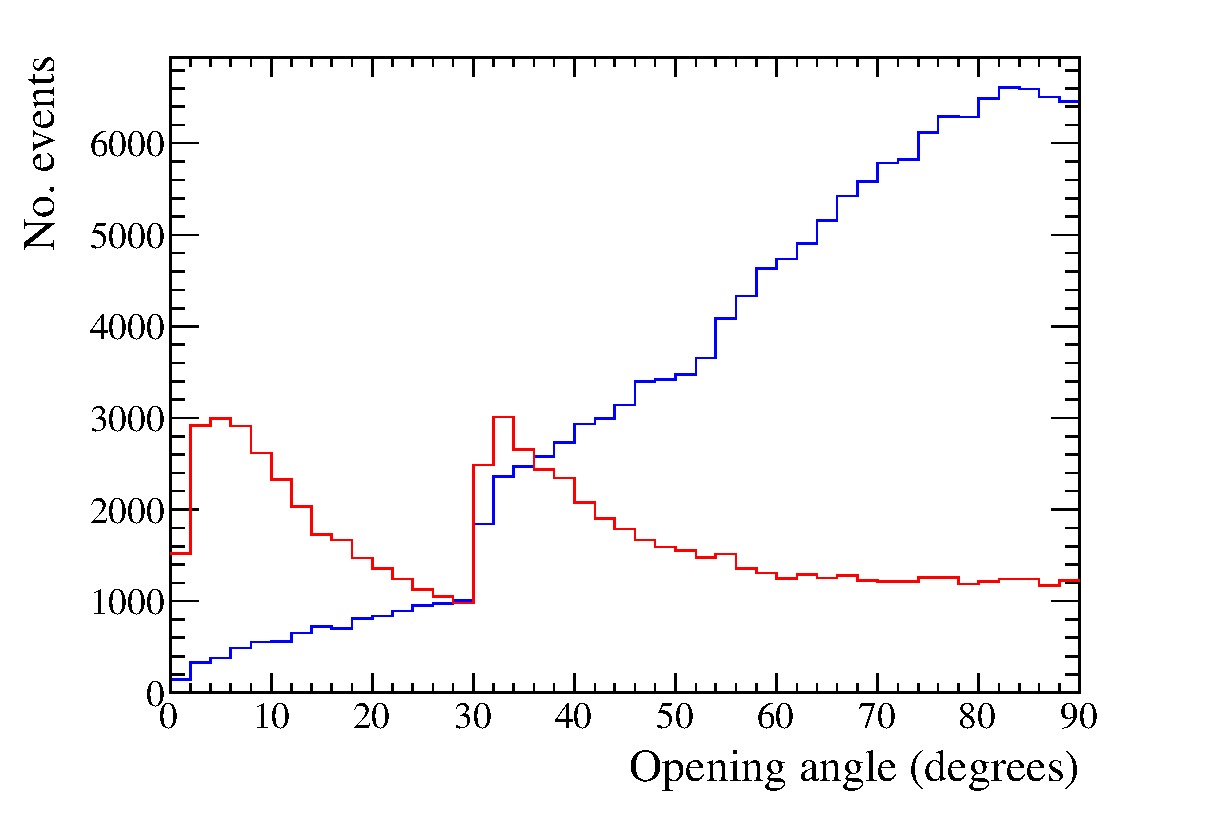
\includegraphics[width=8cm]{images/selection/mc_selection/OpeningAngle_2Prong_Barrel.eps} \label{fig:Sel2OpeningAngleBarrel}}
  \subfloat[DS ECals.]{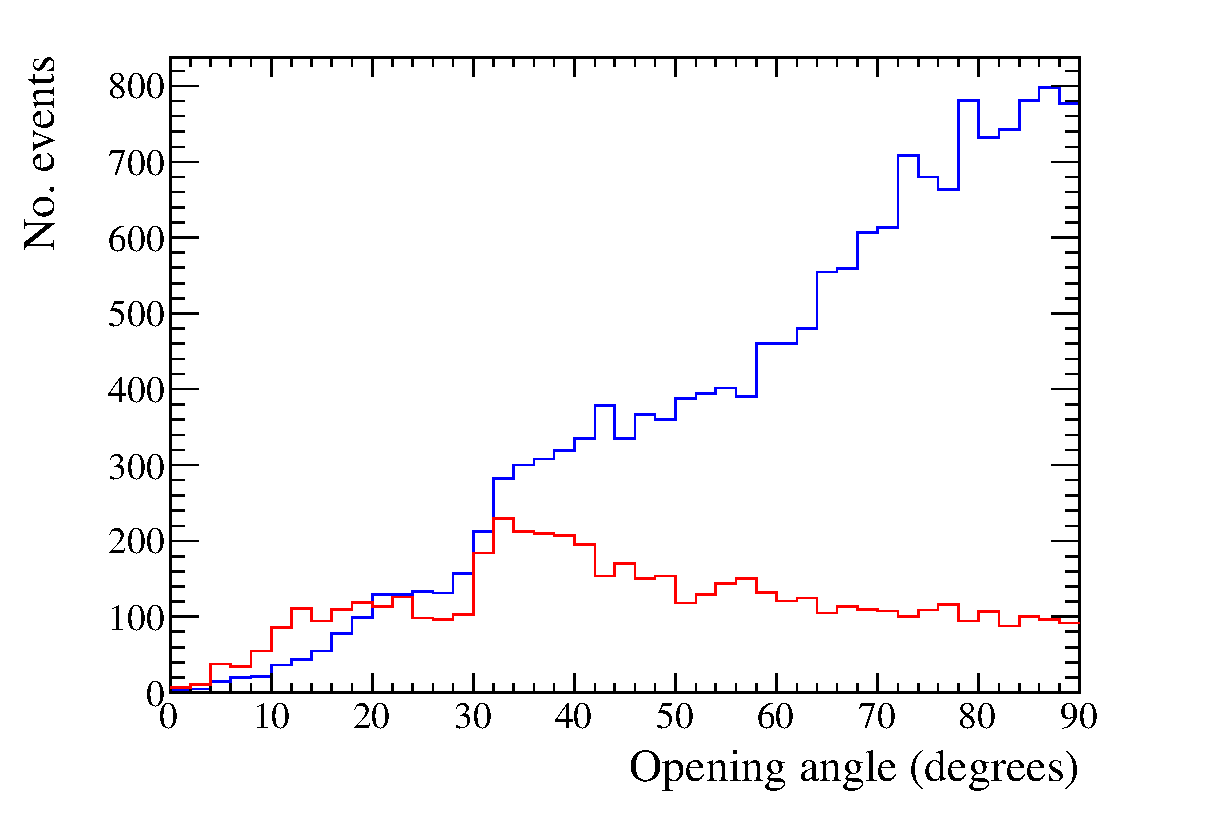
\includegraphics[width=8cm]{images/selection/mc_selection/OpeningAngle_2Prong_DS.eps}\label{fig:Sel2OpeningAngleDS}}
  \caption{The opening angle subtended by the constituents prongs for the 2 prong topology.  Signal and background events are the blue and red histograms respectively.}
  \label{fig:Sel2OpeningAngle}
\end{figure}
The signal and background separation provided by the subtended opening angle for the 2 prong topology is shown in Fig.~\ref{fig:Sel2OpeningAngle}.  While the barrel ECal sees more separation power in the opening angle, it should be clear from Fig.~\ref{fig:Sel2OpeningAngleBarrel} and Fig.~\ref{fig:Sel2OpeningAngleDS} that events should only be selected if their opening angle is bigger than some threshold.  To find this threshold, a test cut was systematically varied between 0$^\circ$ and 90$^\circ$ in 1$^\circ$ increments.  At each increment, the number of events with an opening angle larger than the test cut was recorded and $\phi_2^{\textrm{selection}}$ subsequently calculated.  An example of the variation in $\phi_2^{\textrm{selection}}$ is shown in Fig.~\ref{fig:Sel2OpeningAngleBarrelFOM} for the barrel ECal.  A maximum in $\phi_2^{\textrm{selection}}$ is clearly found which shows that the opening angle is a good discriminator and that the method works.  By applying this method to 2 prong events, events are only selected if the subtended opening angle is greater than 34$^\circ$ for the barrel ECal or greater than 21$^\circ$ for the DS ECal.
\begin{figure}
  \centering
  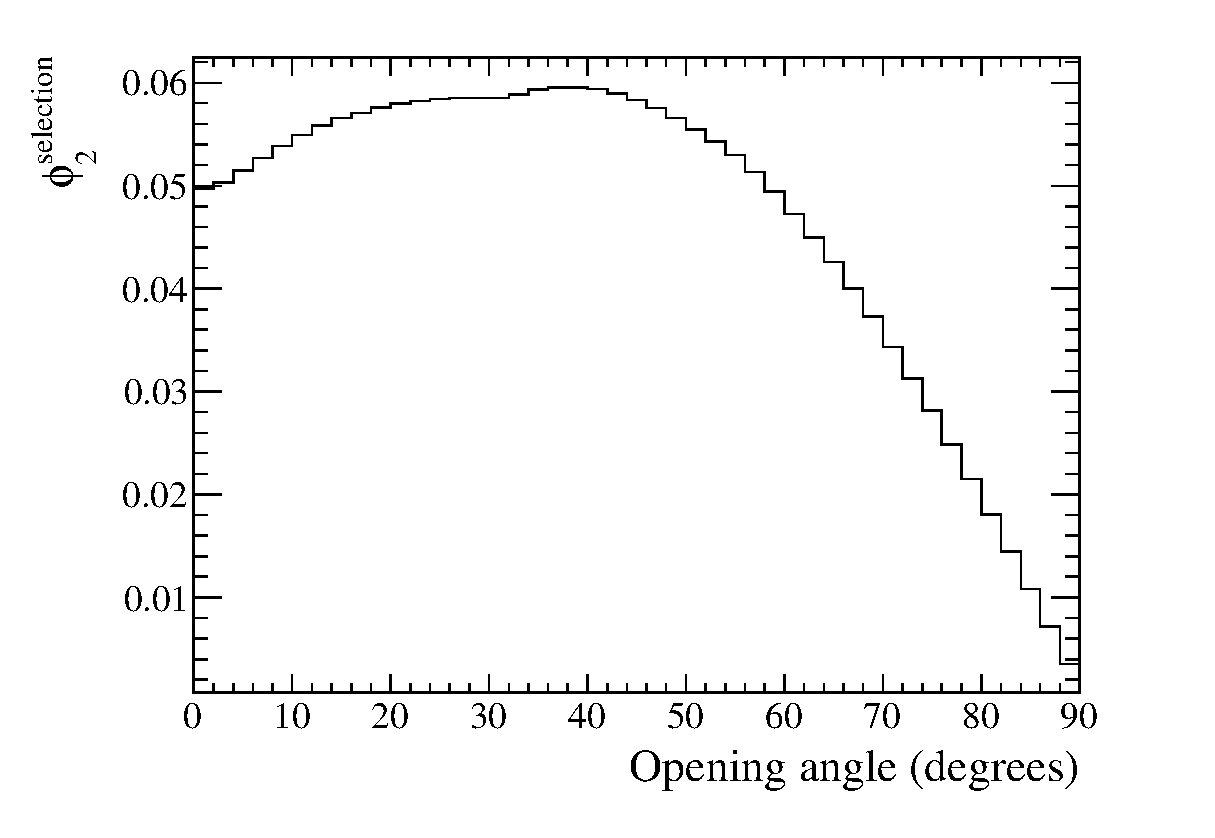
\includegraphics[width=12cm]{images/selection/mc_selection/OpeningAngle_FOM_2Prong_Barrel.eps}
  \caption{$\phi_2^{\textrm{selection}}$ as a function of the opening angle cut for the 2 prong topology in the barrel ECal.}
  \label{fig:Sel2OpeningAngleBarrelFOM}
\end{figure}
Similar information should be available for the higher prong topologies.  However it is not as trivial to define an opening angle in such situations.  The chosen variable for the 3 prong topology is the summed opening angle for every pairwise combination of the constituent prongs.  The signal and background separation for this summed opening angle is shown in Fig.~\ref{fig:Sel3OpeningAngle}.  The cut development process used here was identical to the one used for the 2 prong topology.  The study suggested that events should only be selected if their summed opening angle is greater than 81$^\circ$ for the barrel ECal and 49$^\circ$ for the DS ECal. 
\begin{figure}%
  \centering
  \subfloat[Barrel ECals.]{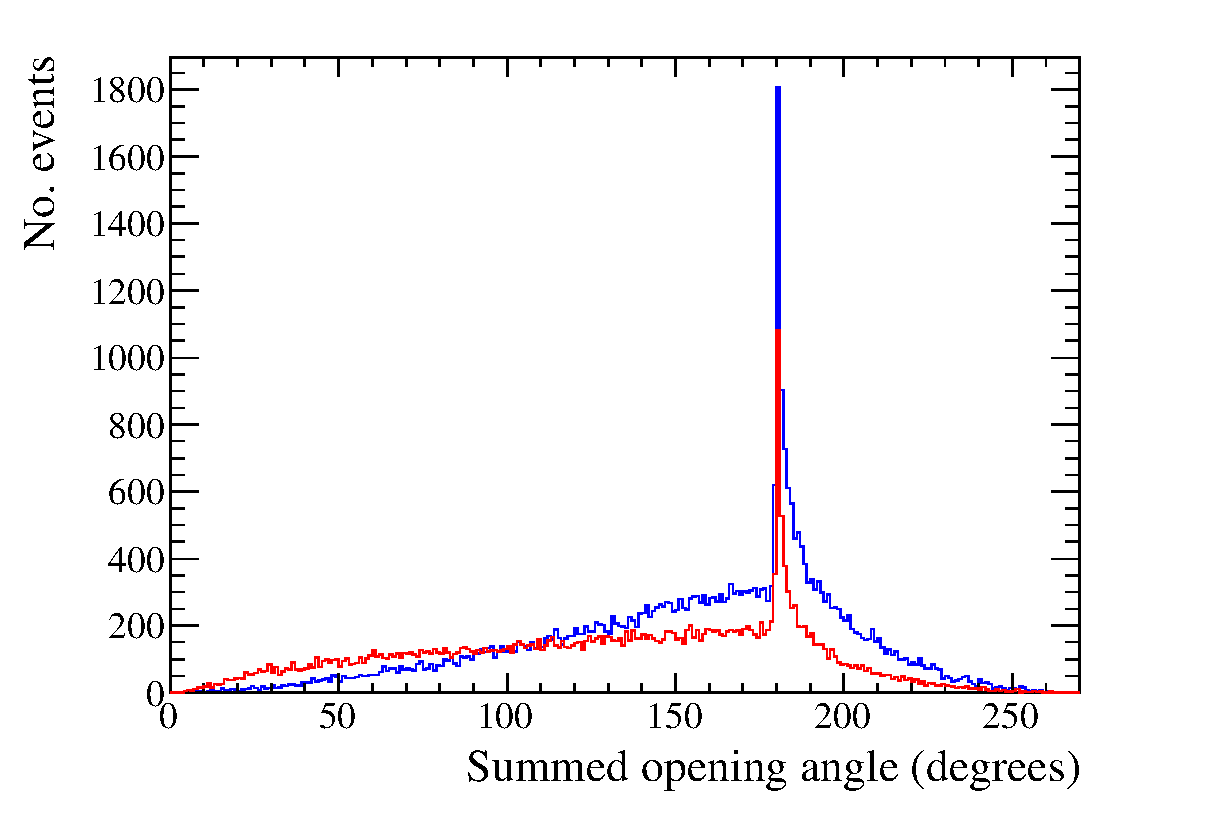
\includegraphics[width=8cm]{images/selection/mc_selection/OpeningAngle_3Prong_Barrel.eps} \label{fig:Sel3OpeningAngleBarrel}}
  \subfloat[DS ECal.]{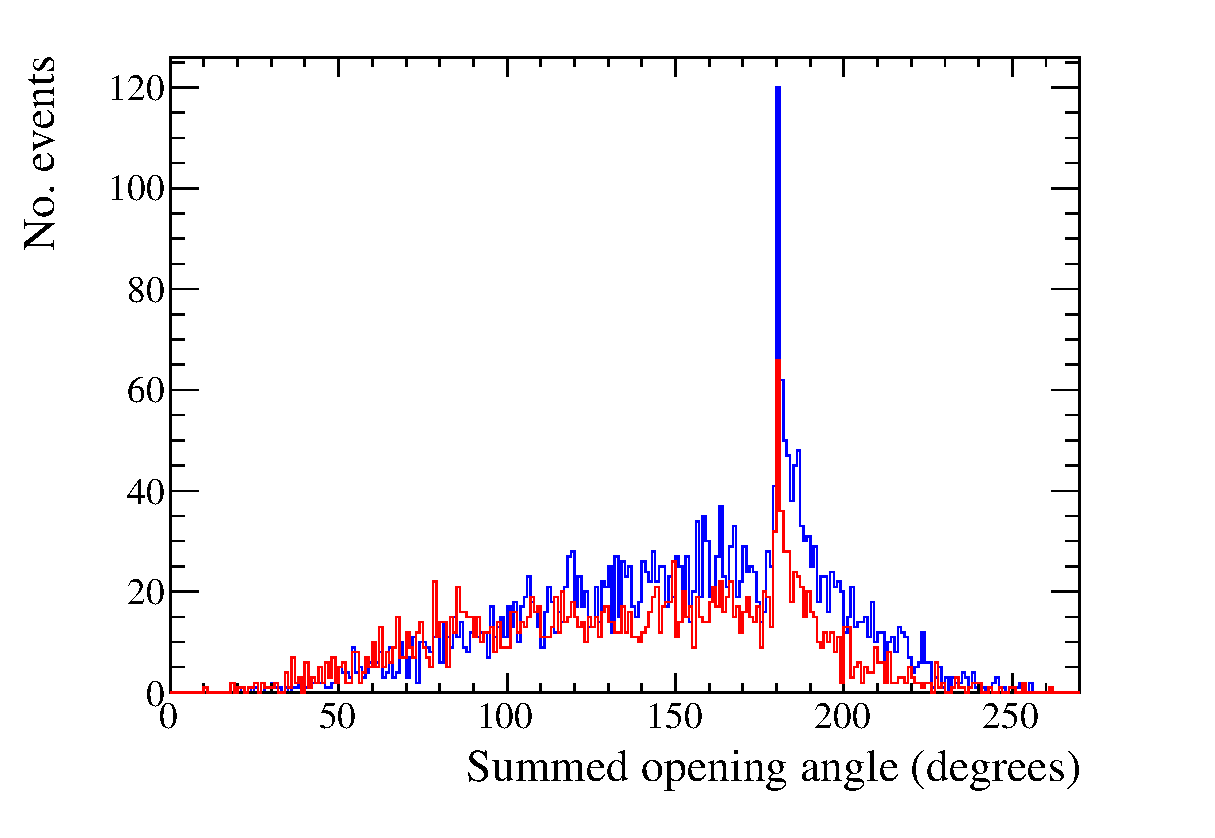
\includegraphics[width=8cm]{images/selection/mc_selection/OpeningAngle_3Prong_DS.eps}\label{fig:Sel3OpeningAngleDS}}
  \caption{The summed opening angle subtended by every pairwise combination of the constituents prongs for the 3 prong topology.  Signal and background events are the blue and red histograms respectively.}
  \label{fig:Sel3OpeningAngle}
\end{figure}
The cuts found by this study are summarised in table~\ref{table:SelOpeningAngle}.
\begin{table}[b!]
  \begin{tabular}{ c l l }
    Prong topology & Barrel cuts (degrees) & DS cuts (degrees) \\ \hline \hline
    2 & $>34$ & $>21$ \\
    3 & $>81$ & $>49$ \\
  \end{tabular}
  \caption{The definitions of the opening angle cuts.}
  \label{table:SelOpeningAngle}
\end{table}
\subsubsection{Entering background cut}
\label{subsubsec:EnteringBackgroundCut}
The fifth cut, simply called the 'entering background' cut, uses the prong multiplicity aspect of a vertex to reject events that enter the ECal and then mimic a signal vertex.  The cut requires at least two constituent prongs to work, so the 1 prong topology is unaffected by this.  The idea is fairly simple: for each vertex, check if any of the prongs have an end which is upstream of the reconstructed vertex position.  If so, it may be an entering background and could need rejecting.  The position of the upstream prong end is key, as the cut should not reject every event which has an apparent backwards going track.  So, the cut checks whether the upstream prong end is outside of the host ECal fiducial volume.  As described in section~\ref{subsubsec:FVCut}, each ECal module uses two fiducial volumes.  The 2+ prong fiducial volume would be of little use in this situation as the only strict face definition is for the downstream end of each ECal module.  This motivates the use of the 1 prong fiducial volume for this cut.  This cut is physically motivated and relies on parameters which have already been tuned.  So, this cut requires no tuning to operate.

\subsubsection{Most upstream vertex}
\label{subsubsec:MostUpstreamCut}
The sixth and final cut implemented is motivated by the beam kinematics.  As discussed in section~\ref{sec:MonteCarloSample}, the expected pileup per beam bunch is small.  As the reconstruction outputs events in buckets, the same philosophy can be used here; there should only be one signal event per bucket.  The assumption used for this cut is any secondary interactions are likely to happen downstream of the interaction.  So, the cut selects the most upstream remaining vertex in the beam bucket.  As with the 'entering background' cut, the selection of the most upstream vertex requires no tuning to operate.

\subsection{Performance of the selection}
\label{subsec:SelectionPerformance}
Now that the cuts have been identified, their performance can be assessed.  To do this, the Monte Carlo sample was processed through the selection and the event composition assessed at each stage.  As each cut was focused on a specific topology, it is important to check the effect of the cuts on each topology.  The first check looks at the event survival as a function of the cuts for each topology.  These checks are shown in Fig.~\ref{fig:SelEventSurvivalBarrel} and Fig.~\ref{fig:SelEventSurvivalDS} for the barrel and DS ECals respectively.  Each bin in both figures shows how many events survive after the cut has been applied.  For example, the FV bin in all of the figures shows how many events remain after applying the fiducial volume cut.  As the 'most upstream' cut is the final cut in the selection, the final bin shows how many events remain after the full selection has been applied.  The main piece of information shown is that the backgrounds are being rejected at a much higher rate than the signal, resulting in a selected sample that is mostly signal.
\begin{figure}
\begin{minipage}{.5\linewidth}
  \centering
  \subfloat[1 prong topology.]{\label{fig:Sel1EventSurvivalBarrel}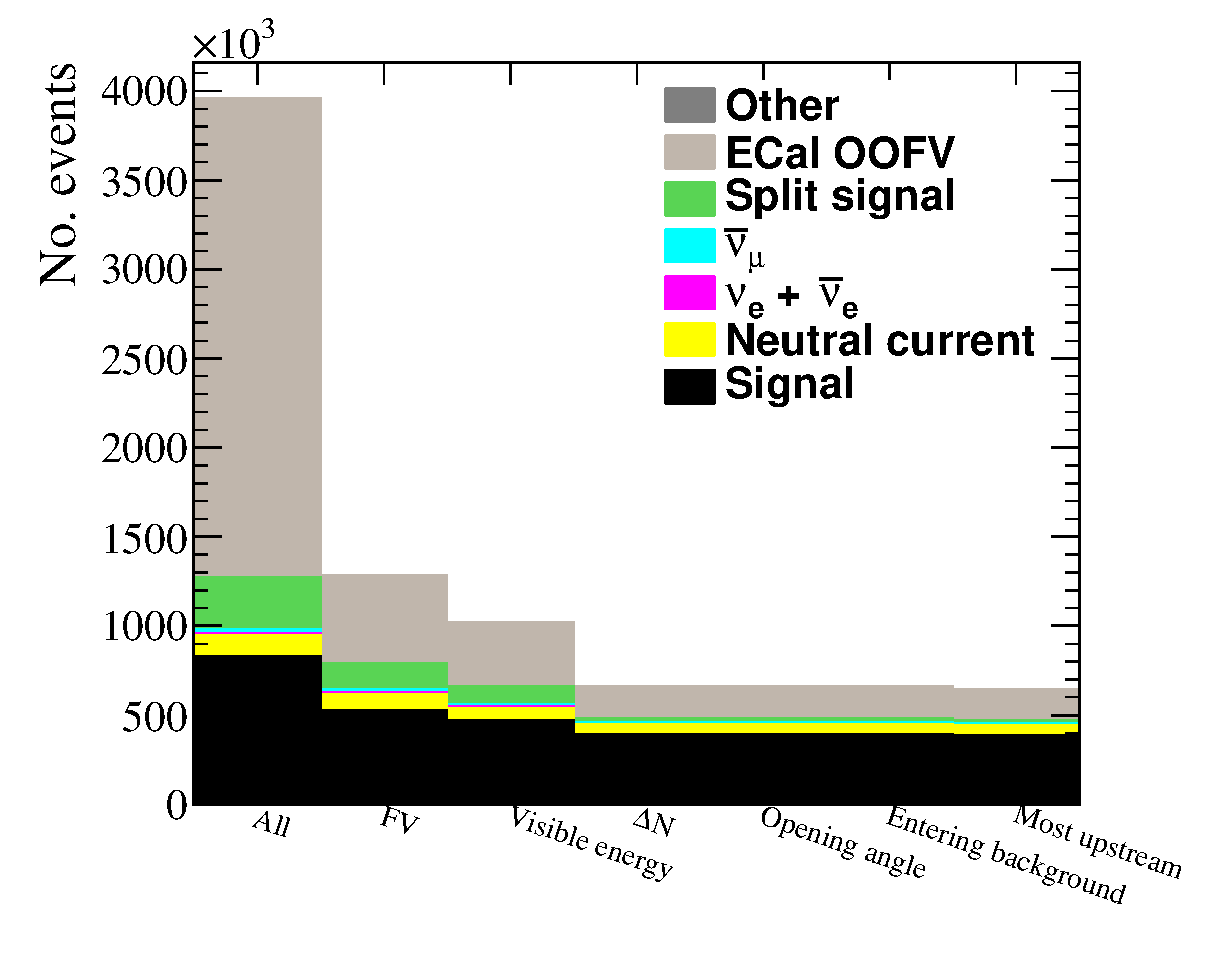
\includegraphics[width=7.5cm]{images/selection/selection_performance/CutSurvival_1Prong_Barrel.eps}}
\end{minipage}%
\begin{minipage}{.5\linewidth}
\centering
\subfloat[2 prong topology.]{\label{fig:Sel2EventSurvivalBarrel}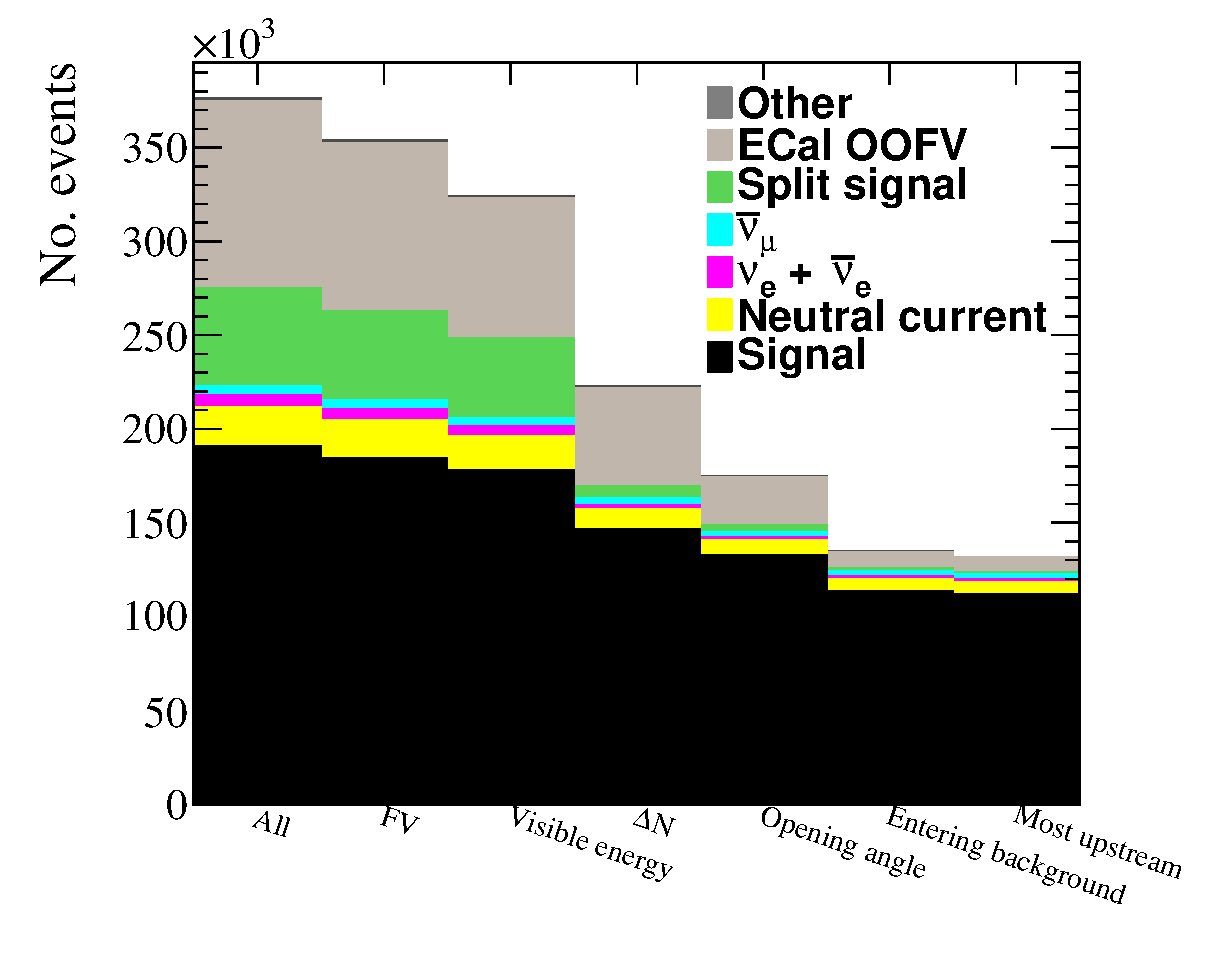
\includegraphics[width=7.5cm]{images/selection/selection_performance/CutSurvival_2Prong_Barrel.eps}}
\end{minipage}\par\medskip
\begin{minipage}{.5\linewidth}
  \centering
  \subfloat[3 prong topology.]{\label{fig:Sel3EventSurvivalBarrel}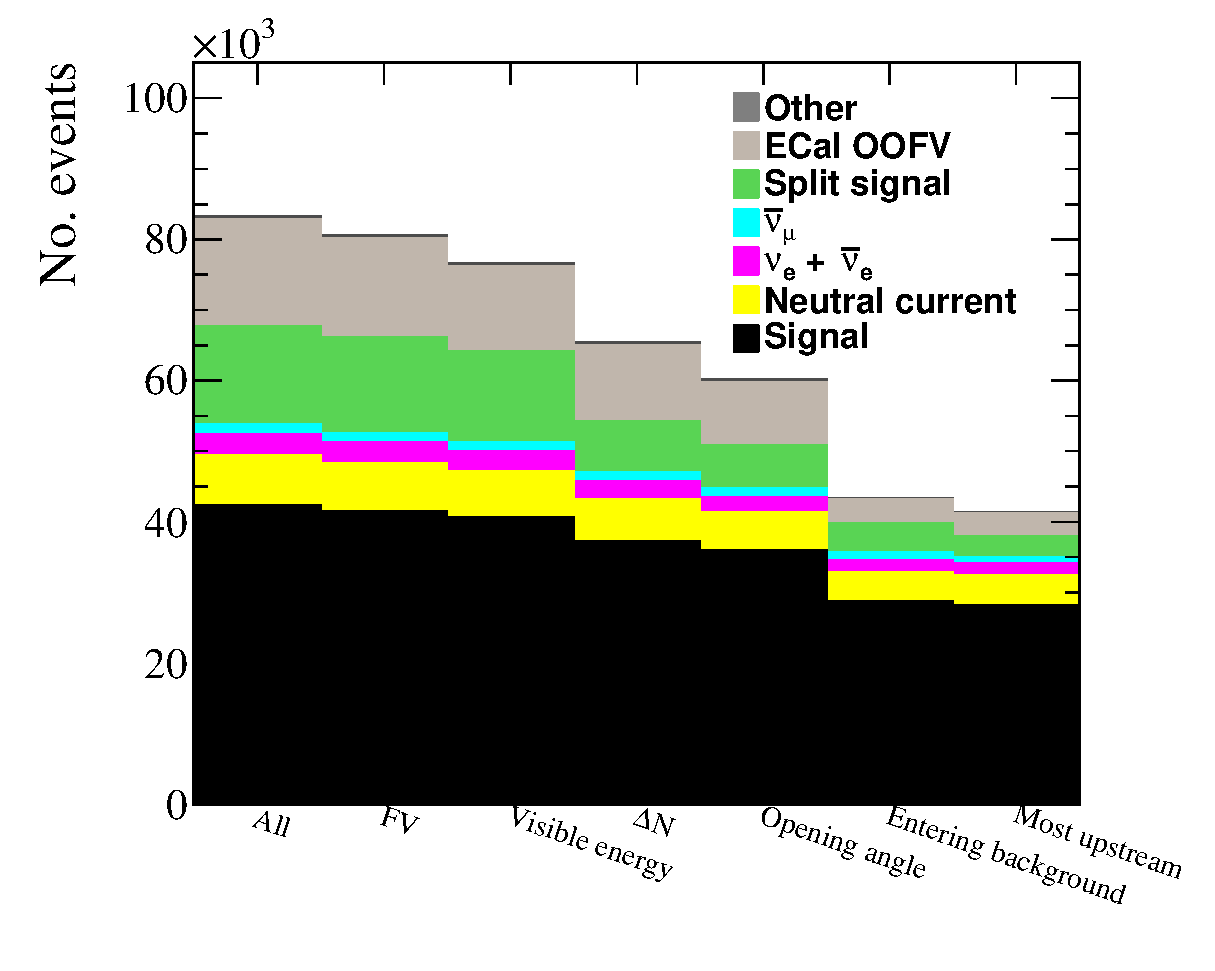
\includegraphics[width=7.5cm]{images/selection/selection_performance/CutSurvival_3Prong_Barrel.eps}}
\end{minipage}%
\begin{minipage}{.5\linewidth}
\centering
\subfloat[4+ prong topology.]{\label{fig:Sel4EventSurvivalBarrel}\includegraphics[width=7.5cm]{images/selection/selection_performance/CutSurvival_4Prong_Barrel.eps}}
\end{minipage}\par\medskip
\caption{Event survival as a function of the cuts for all topologies in the barrel ECal.  Each bin refers to the number of events after a cut has been applied.}
\label{fig:SelEventSurvivalBarrel}
\end{figure}
\begin{figure}
\begin{minipage}{.5\linewidth}
  \centering
  \subfloat[1 prong topology.]{\label{fig:Sel1EventSurvivalDS}\includegraphics[width=7.5cm]{images/selection/selection_performance/CutSurvival_1Prong_DS.eps}}
\end{minipage}%
\begin{minipage}{.5\linewidth}
\centering
\subfloat[2 prong topology.]{\label{fig:Sel2EventSurvivalDS}\includegraphics[width=7.5cm]{images/selection/selection_performance/CutSurvival_2Prong_DS.eps}}
\end{minipage}\par\medskip
\begin{minipage}{.5\linewidth}
  \centering
  \subfloat[3 prong topology.]{\label{fig:Sel3EventSurvivalDS}\includegraphics[width=7.5cm]{images/selection/selection_performance/CutSurvival_3Prong_DS.eps}}
\end{minipage}%
\begin{minipage}{.5\linewidth}
\centering
\subfloat[4+ prong topology.]{\label{fig:Sel4EventSurvivalDS}\includegraphics[width=7.5cm]{images/selection/selection_performance/CutSurvival_4Prong_DS.eps}}
\end{minipage}\par\medskip
\caption{Event survival as a function of the cuts for all topologies in the DS ECal.  Each bin refers to the number of events after a cut has been applied.}
\label{fig:SelEventSurvivalDS}
\end{figure}
\newline
\newline
While Fig.~\ref{fig:SelEventSurvivalBarrel} and Fig.~\ref{fig:SelEventSurvivalDS} shows that the cuts are successfully rejecting background while retaining signal, it is not clear what particle species are rejected.  It is important to check this so that the developed selection is understood.  The background type which is rejected at the highest rate is the ECal OOFV background so it is sufficient to study the particle composition of this to understand the selection's ability to reject particles.  The particle type is defined by looking at which simulated particles contributed to the ECal cluster as whole.  The particle which deposited the highest amount of energy is accepted as the one which created the ECal cluster.  The ECal OOFV event survival as a function of the cuts is shown in Fig.~\ref{fig:SelOOFVEventSurvivalBarrel} and Fig.~\ref{fig:SelOOFVEventSurvivalDS} for the barrel and DS ECal respectively.  For each prong topology, the ECal OOFV events are separated into the main particle types which constitute the ECal OOFV background.  It is clear that the cuts are rejecting the particle species that one would expect them to reject.  For example, the fiducial volume cut in the 1 prong topology almost exclusively rejects entering MIPs.  The visible energy and $\Delta N$ cuts worth together as an effective particle shower tagger to reject $e^\pm$ and $\gamma$ particles.  The opening angle and entering background cuts work as an additional MIP rejector in cases where the track merging was unsuccessful.  The composition of the ECal OOFV background has interesting features, regardless of the cuts applied.  Specifically, the particle species varies to a great degree between each prong topology.  For example, the 1 prong and 2 prong topologies in the barrel ECals (Fig.~\ref{fig:Sel1OOFVEventSurvivalBarrel} and Fig.~\ref{fig:Sel2OOFVEventSurvivalBarrel}) see a muon dominated ECal OOFV background.  Whereas, the 3 prong and 4+ prong topologies see a very different background which is $\pi^\pm$ dominated.  The natural separation provided by the topologies should allow investigation of a specific particle species if required by any future analyser.
\begin{figure}
\begin{minipage}{.5\linewidth}
  \centering
  \subfloat[1 prong topology.]{\label{fig:Sel1OOFVEventSurvivalBarrel}\includegraphics[width=7.5cm]{images/selection/selection_performance/OOFVCutSurvival_1Prong_Barrel.eps}}
\end{minipage}%
\begin{minipage}{.5\linewidth}
\centering
\subfloat[2 prong topology.]{\label{fig:Sel2OOFVEventSurvivalBarrel}\includegraphics[width=7.5cm]{images/selection/selection_performance/OOFVCutSurvival_2Prong_Barrel.eps}}
\end{minipage}\par\medskip
\begin{minipage}{.5\linewidth}
  \centering
  \subfloat[3 prong topology.]{\label{fig:Sel3OOFVEventSurvivalBarrel}\includegraphics[width=7.5cm]{images/selection/selection_performance/OOFVCutSurvival_3Prong_Barrel.eps}}
\end{minipage}%
\begin{minipage}{.5\linewidth}
\centering
\subfloat[4+ prong topology.]{\label{fig:Sel4OOFVEventSurvivalBarrel}\includegraphics[width=7.5cm]{images/selection/selection_performance/OOFVCutSurvival_4Prong_Barrel.eps}}
\end{minipage}\par\medskip
\caption{ECal OOFV event survival as a function of the cuts for all topologies in the barrel ECal.  Each bin refers to the number of events after a cut has been applied.}
\label{fig:SelOOFVEventSurvivalBarrel}
\end{figure}
\begin{figure}
\begin{minipage}{.5\linewidth}
  \centering
  \subfloat[1 prong topology.]{\label{fig:Sel1OOFVEventSurvivalDS}\includegraphics[width=7.5cm]{images/selection/selection_performance/OOFVCutSurvival_1Prong_DS.eps}}
\end{minipage}%
\begin{minipage}{.5\linewidth}
\centering
\subfloat[2 prong topology.]{\label{fig:Sel2OOFVEventSurvivalDS}\includegraphics[width=7.5cm]{images/selection/selection_performance/OOFVCutSurvival_2Prong_DS.eps}}
\end{minipage}\par\medskip
\begin{minipage}{.5\linewidth}
  \centering
  \subfloat[3 prong topology.]{\label{fig:Sel3OOFVEventSurvivalDS}\includegraphics[width=7.5cm]{images/selection/selection_performance/OOFVCutSurvival_3Prong_DS.eps}}
\end{minipage}%
\begin{minipage}{.5\linewidth}
\centering
\subfloat[4+ prong topology.]{\label{fig:Sel4OOFVEventSurvivalDS}\includegraphics[width=7.5cm]{images/selection/selection_performance/OOFVCutSurvival_4Prong_DS.eps}}
\end{minipage}\par\medskip
\caption{ECal OOFV event survival as a function of the cuts for all topologies in the DS ECal.  Each bin refers to the number of events after a cut has been applied.}
\label{fig:SelOOFVEventSurvivalDS}
\end{figure}
\newline
\newline
The selection efficiency and purity as a function of the cuts are shown for the barrel ECal and DS ECal in Fig.~\ref{fig:SelEffPurCutLevelBarrel} and Fig.~\ref{fig:SelEffPurCutLevelDS} respectively.  Every cut which is relevant to a prong topology has an expected effect, the purity of the sample increases while the efficiency decreases.  What is not so clear from the distributions is whether the tuning metric, $\phi^{\textrm{selection}}$, increases as a function of the cuts.  So, $\phi^{\textrm{selection}}$ is shown in a similar manner for the barrel and DS ECal in Fig.~\ref{fig:SelFOMCutLevelBarrel} and Fig.~\ref{fig:SelFOMCutLevelDS} respectively.  The tuning metric optimisation in both the barrel and DS ECal shows some interesting features.  Firstly, in the barrel, it is clear that for the 1 prong and 2 prong topologies, every applied cut shows a clearly increasing $\phi^{\textrm{selection}}$.  Unfortunately, this is not the case for the 3 prong and 4+ prong topologies.  Specifically, the entering background cut degrades the value of $\phi^{\textrm{selection}}$.  This is most obvious in the 4+ prong topology\Yoshi{; however,}{ADDRESSED - was ``, however''} it has already been stated that this topology is effectively an overflow bin and is being included more for completeness.  What is perhaps more concerning is the degradation of $\phi^{\textrm{selection}}$ in the 3 prong topology.  Fortunately, the decrease in $\phi^{\textrm{selection}}$ is small when the entering background cut is applied and the change is well within error.  It is important to bear in mind that $\phi^{\textrm{selection}}$ is used as a tuning guide and small deviations from the optimisation process are allowed.  So, it was decided that the entering background cut would remain in place for both the 3 prong and 4+ prong topologies.  The $\phi^{\textrm{selection}}$ distribution in the DS ECal shows some similar and some different features to that of the barrel.  As with the barrel ECal case, $\phi^{\textrm{selection}}$ clearly increases as a function of the cuts for the 1 prong and 2 prong topologies.  Unlike the barrel ECal, there is also an increase in $\phi^{\textrm{selection}}$ when applying the entering background cut to the 3 and 4+ prong topologies.  However, there is a minor decrease in $\phi^{\textrm{selection}}$ when selecting the most upstream vertex.  It is not wholly surprising that this is the case as the DS ECal is the most downstream detector in ND280.  Such a cut can easily cause a bias where events in the barrel are generally preferred because of their extent in the global $Z$ direction.  Fortunately, this effect is very minor and also well within error.  
\begin{figure}
\begin{minipage}{.5\linewidth}
  \centering
  \subfloat[1 prong topology.]{\label{fig:Sel1EffPurCutLevelBarrel}\includegraphics[width=7.5cm]{images/selection/selection_performance/EffPur_CutLevel_1Prong_Barrel.eps}}
\end{minipage}%
\begin{minipage}{.5\linewidth}
\centering
\subfloat[2 prong topology.]{\label{fig:Sel2EffPurCutLevelBarrel}\includegraphics[width=7.5cm]{images/selection/selection_performance/EffPur_CutLevel_2Prong_Barrel.eps}}
\end{minipage}\par\medskip
\begin{minipage}{.5\linewidth}
  \centering
  \subfloat[3 prong topology.]{\label{fig:Sel3EffPurCutLevelBarrel}\includegraphics[width=7.5cm]{images/selection/selection_performance/EffPur_CutLevel_3Prong_Barrel.eps}}
\end{minipage}%
\begin{minipage}{.5\linewidth}
\centering
\subfloat[4+ prong topology.]{\label{fig:Sel4EffPurCutLevelBarrel}\includegraphics[width=7.5cm]{images/selection/selection_performance/EffPur_CutLevel_4Prong_Barrel.eps}}
\end{minipage}\par\medskip
\caption{The selection efficiency (black) and purity (red) as a function of the cuts in the barrel ECal.  Each bin refers to the efficiency and purity after a cut has been applied.}
\label{fig:SelEffPurCutLevelBarrel}
\end{figure}
\begin{figure}
\begin{minipage}{.5\linewidth}
  \centering
  \subfloat[1 prong topology.]{\label{fig:Sel1EffPurCutLevelDS}\includegraphics[width=7.5cm]{images/selection/selection_performance/EffPur_CutLevel_1Prong_DS.eps}}
\end{minipage}%
\begin{minipage}{.5\linewidth}
\centering
\subfloat[2 prong topology.]{\label{fig:Sel2EffPurCutLevelDS}\includegraphics[width=7.5cm]{images/selection/selection_performance/EffPur_CutLevel_2Prong_DS.eps}}
\end{minipage}\par\medskip
\begin{minipage}{.5\linewidth}
  \centering
  \subfloat[3 prong topology.]{\label{fig:Sel3EffPurCutLevelDS}\includegraphics[width=7.5cm]{images/selection/selection_performance/EffPur_CutLevel_3Prong_DS.eps}}
\end{minipage}%
\begin{minipage}{.5\linewidth}
\centering
\subfloat[4+ prong topology.]{\label{fig:Sel4EffPurCutLevelDS}\includegraphics[width=7.5cm]{images/selection/selection_performance/EffPur_CutLevel_4Prong_DS.eps}}
\end{minipage}\par\medskip
\caption{The selection efficiency (black) and purity (red) as a function of the cuts in the DS ECal.  Each bin refers to the efficiency and purity after a cut has been applied.}
\label{fig:SelEffPurCutLevelDS}
\end{figure}
\begin{figure}
\begin{minipage}{.5\linewidth}
  \centering
  \subfloat[1 prong topology.]{\label{fig:Sel1FOMCutLevelBarrel}\includegraphics[width=7.5cm]{images/selection/selection_performance/FOM_CutLevel_1Prong_Barrel.eps}}
\end{minipage}%
\begin{minipage}{.5\linewidth}
\centering
\subfloat[2 prong topology.]{\label{fig:Sel2FOMCutLevelBarrel}\includegraphics[width=7.5cm]{images/selection/selection_performance/FOM_CutLevel_2Prong_Barrel.eps}}
\end{minipage}\par\medskip
\begin{minipage}{.5\linewidth}
  \centering
  \subfloat[3 prong topology.]{\label{fig:Sel3FOMCutLevelBarrel}\includegraphics[width=7.5cm]{images/selection/selection_performance/FOM_CutLevel_3Prong_Barrel.eps}}
\end{minipage}%
\begin{minipage}{.5\linewidth}
\centering
\subfloat[4+ prong topology.]{\label{fig:Sel4FOMCutLevelBarrel}\includegraphics[width=7.5cm]{images/selection/selection_performance/FOM_CutLevel_4Prong_Barrel.eps}}
\end{minipage}\par\medskip
\caption{$\phi^{\textrm{selection}}$ as a function of the cuts in the barrel ECal.  Each bin refers to the value of $\phi^{\textrm{selection}}$ after a cut has been applied.}
\label{fig:SelFOMCutLevelBarrel}
\end{figure}
\begin{figure}
\begin{minipage}{.5\linewidth}
  \centering
  \subfloat[1 prong topology.]{\label{fig:Sel1FOMCutLevelDS}\includegraphics[width=7.5cm]{images/selection/selection_performance/FOM_CutLevel_1Prong_DS.eps}}
\end{minipage}%
\begin{minipage}{.5\linewidth}
\centering
\subfloat[2 prong topology.]{\label{fig:Sel2FOMCutLevelDS}\includegraphics[width=7.5cm]{images/selection/selection_performance/FOM_CutLevel_2Prong_DS.eps}}
\end{minipage}\par\medskip
\begin{minipage}{.5\linewidth}
  \centering
  \subfloat[3 prong topology.]{\label{fig:Sel3FOMCutLevelDS}\includegraphics[width=7.5cm]{images/selection/selection_performance/FOM_CutLevel_3Prong_DS.eps}}
\end{minipage}%
\begin{minipage}{.5\linewidth}
\centering
\subfloat[4+ prong topology.]{\label{fig:Sel4FOMCutLevelDS}\includegraphics[width=7.5cm]{images/selection/selection_performance/FOM_CutLevel_4Prong_DS.eps}}
\end{minipage}\par\medskip
\caption{$\phi^{\textrm{selection}}$ as a function of the cuts in the DS ECal.  Each bin refers to the value of $\phi^{\textrm{selection}}$ after a cut has been applied.}
\label{fig:SelFOMCutLevelDS}
\end{figure}
\newline
\newline
The cross-section measurement presented in this analysis in an inclusive measurement.  This means that the neutrino interaction cross-section needs to be measured without bias across the J-PARC beam energy range.  All of the performance checks presented so far have only assessed each prong topology individually.  So, the final check is to assess how the selection performs after combining the topologies together.  The selection efficiency and purity after combining the topologies is shown in Fig.~\ref{fig:EffPurSummedTopologies}.  For both the barrel ECal and DS ECal, there is a clear dependence of the purity on the neutrino energy.  However, this should be expected.  It is clear that the purity decreases as the neutrino energy increases which can be explained by the self-shielding effect of the ECal.  In the low energy regime, the ECal OOFV background is suppressed because there is insufficient energy to either penetrate the ECal or deposit enough energy to allow cluster reconstruction.  As the background energy increases, the suppression is lifted, resulting in a decrease in the selection purity.  The key piece of information shown in Fig.~\ref{fig:EffPurSummedTopologies} is the selection efficiency.  As described above, it is of vital importance that the selection does not introduce a bias which measures one energy regime more than another.  The flatness of the efficiency distributions for both the barrel ECal and DS ECal shows this is not the case which means the selection presented here would be suitable for a CC-inclusive measurement.
\begin{figure}
  \centering
  \subfloat[Barrel ECals.]{\includegraphics[width=8cm]{images/selection/selection_performance/EffPur_SummedTopologies_Barrel.eps} \label{fig:EffPurSummedTopologiesBarrel}}
  \subfloat[DS ECal.]{\includegraphics[width=8cm]{images/selection/selection_performance/EffPur_SummedTopologies_DS.eps} \label{fig:EffPurSummedTopologiesDS}}
  \caption{The selection efficiency (black) and purity (red) for the combined prong topologies as a function of neutrino energy.}
  \label{fig:EffPurSummedTopologies}
\end{figure}
\newline
\newline
\begin{figure}
  \centering
  \subfloat[Barrel ECals.]{\includegraphics[width=8cm]{images/selection/mc_selection/ProngStack_Barrel_Selected.eps} \label{fig:ProngStackBarrelSelected}}
  \subfloat[DS ECal.]{\includegraphics[width=8cm]{images/selection/mc_selection/ProngStack_DS_Selected.eps} \label{fig:ProngStackDSSelected}}
  \caption{The number of selected events in the Monte Carlo sample, separated out into the prong topologies.  Each event is categorised by the associated truth information from the simulation.}
  \label{fig:ProngStackSelected}
\end{figure}
The number of selected events for each prong topology is shown in Fig.~\ref{fig:ProngStackSelected}, with each topology broken down by truth categories.  For both the barrel and DS ECal, signal events dominate each prong topology.  The most impure topology for both detectors is the 1 prong topology.  This is primarily due to having an insufficient number of prongs to really benefit from what the reconstruction can provide.  Despite this, it is clear that the selection results in a pure sample of events.  
\newline
\newline
The selection efficiencies and purities for each prong topology are shown in table~\ref{table:SelEfficiency} and table~\ref{table:SelPurity} respectively.  The final purities and efficiencies are generally good.  
%The only concern is the 1 prong topology efficiency in the barrel ECal which is notably lower than all other efficiencies.  The main reason for the low efficiency is the strict fiducial volumes defined for each ECal module.  Generally speaking, this low efficiency may cause a problem if there is a significant amount of signal migration from the 2 prong topology which is more efficient.  It is important to address this when assessing systematic uncertainties for the analysis.
\begin{table}
  \begin{tabular}{ c c c c c }
    ECal & 1 prong topology & 2 prong topology & 3 prong topology & 4+ prong topology \\
    module & efficiency ($\%$)& efficiency ($\%$)& efficiency ($\%$)& efficiency ($\%$) \\ \hline \hline
    Barrel & 46.8 & 58.7 & 66.5 & 66.3 \\
    DS & 59.0 & 64.2 & 62.3 & 60.4\\
  \end{tabular}
  \caption{The selection efficiencies for each prong topology and ECal module.}
  \label{table:SelEfficiency}
\end{table}
\begin{table}
  \begin{tabular}{ c c c c c }
    ECal & 1 prong topology & 2 prong topology & 3 prong topology & 4+ prong topology \\
    module & purity ($\%$)& purity ($\%$)& purity ($\%$)& purity ($\%$) \\ \hline \hline
    Barrel & 60.3 & 85.0 & 68.5 & 63.0\\
    DS & 69.6 & 87.2 & 72.0 & 67.3\\
  \end{tabular}
  \caption{The selection purities for each prong topology and ECal module.}
  \label{table:SelPurity}
\end{table}
\newline
\newline
The selection efficiency is defined to be 100$\%$ when no cuts have been made.  There are inevitably signal events which are not reconstructed, primarily because the energy is below reconstruction threshold.  It is non-trivial to include these events in an efficiency calculations for a specific prong topology, but it is also unnecessary to do this as the prong topologies are to be summed for the CC-inclusive cross-section measurement.  So, the topology combined efficiency and purity are presented in table~\ref{table:FinalEffPur}.  It is these numbers, along with the sample itself, which are the final output of the Monte Carlo selection.
\begin{table}
  \begin{tabular}{ c c c}
    ECal module & Efficiency ($\%$) & Purity ($\%$) \\ \hline \hline
    Barrel & 42.4 & 64.4 \\
    DS & 53.0  & 72.4 \\
  \end{tabular}
  \caption{The topology combined efficiency and purity.}
  \label{table:FinalEffPur}
\end{table}




%\section{Properties of events in selection}

